
\documentclass{double}
\DeclareMathOperator{\arccot}{arccot}
\begin{document}
\title{Studying $\alpha - \gamma$ coincidence for Am-241 using CSpark's dual channel MCA, and experiments with FPGA}
\author{Spandan Anupam\\%
\href{https://github.com/surelynottrue/}{GitHub}}
\date{%
	\small\itshape School of Physical Sciences\\%
	\normalfont National Institute of Science Education and Research\\[2ex]%
	\normalsize\today}
\maketitle

\begin{multicols*}{2}
\tableofcontents

\section{Objective}
The aim of the experiment is to understand and study
coincidence spectra for the $^{241}$Am sample using the
apparatus that we have around. I will be following the
parent paper \cite{vret}, and will be relying heavily on
Filipe et al's paper \cite{filipe} for the theoretical
front.

\section{Apparatus}
\begin{enumerate}
    \item Am-241 source
    \item CSpark dual channel MCA
    \item Vacuum chamber with an integrated photodiode
    \item Gamma scintillation detector
    \item PHYWE signal preamplifier (for the alpha setup)
    \item PHYWE Multi channel analyser (only for the amplification)
    \item Single channel analyser with an integrated HV power source for the gamma setup
    \item Vacuum pump and monitor
    \item BNC Cables
    \item Aluminum foil and a blackout cover
    \item Platforms
\end{enumerate}

\section{Theory}
\subsection{Field Programmable Gate Array}
In this report, we will be talking mostly about studying alpha gamma coincidence as the title says, but since this project was initially about using the
provided Intel (Alterra) FPGA \cite{alterra}, I will be noting down some of the basics of what we were able to learn and do during our time with the board. Please keep in mind that since what we did concerned Intel IPs and lots of custom code, documenting exactly what we did will require us to write a whole new report just for that. Instead, I will note down why we couldn't go ahead with using a FPGA this time around. 

\subsubsection{Transfer speeds} We tried to work with two
kinds of transfer protocols, RS232 and UDP (ethernet). For
the most part, we understood what RS232 does \cite{fpga}, and were able to implement the transfer, and capture side of things quite smoothly. The thing about this is though, that RS232 supports $10,473$ bits per second of transfer speeds. Meaning we can only send one bit per microsecond. This is absolutely not useful for our cause, as we need nanosecond transfer speeds, which is possible in ethernet implementations.

We couldn't give much time for the ethernet implementation, instead, we were able to find an elegant implementation of the same, and were able to confirm that this is infact, quite possible. This is of no use though, because we had one more roadblock that made us abandon this avenue.

\subsubsection{Analog to digital conversion} We must understand that for getting data from the amplifier to the FPGA, we need to convert the base 10 voltage values to base 2 values that can be read by the GPIO pins on the board itself. But for that purpose, we will need a high speed ADC, which we unfortunately did not have. If we interface a say 13 bit ADC to the GPIO header, we can then quite easily set bin boundaries and make a MCA on the FPGA itself, which would be quite fast. We have submitted suggestions for ADCs, which can be included in the experiments that may be conducted in the next semester.


The code for all of this, can be found on my
\href{https://github.com/surelynottrue/coincidence}{repository} and the \href{https://github.com/alexforencich/verilog-ethernet/}{\texttt{verilog-ethernet} repository} authored by Alex Forencich.

\subsection{Amerecium Decay}
$^{241}$Am has quite a number of possible energies for the
alpha particle, while the decay to $^{237}$Np is being
completed. Each possibility here, will be associated with a
different excited state of $^{237}$Np, which is then
deexcited, while releasing a gamma particle of the
corresponding energy. The decay scheme is represented in
figure below.
\begin{figure}[H]
	\centering
	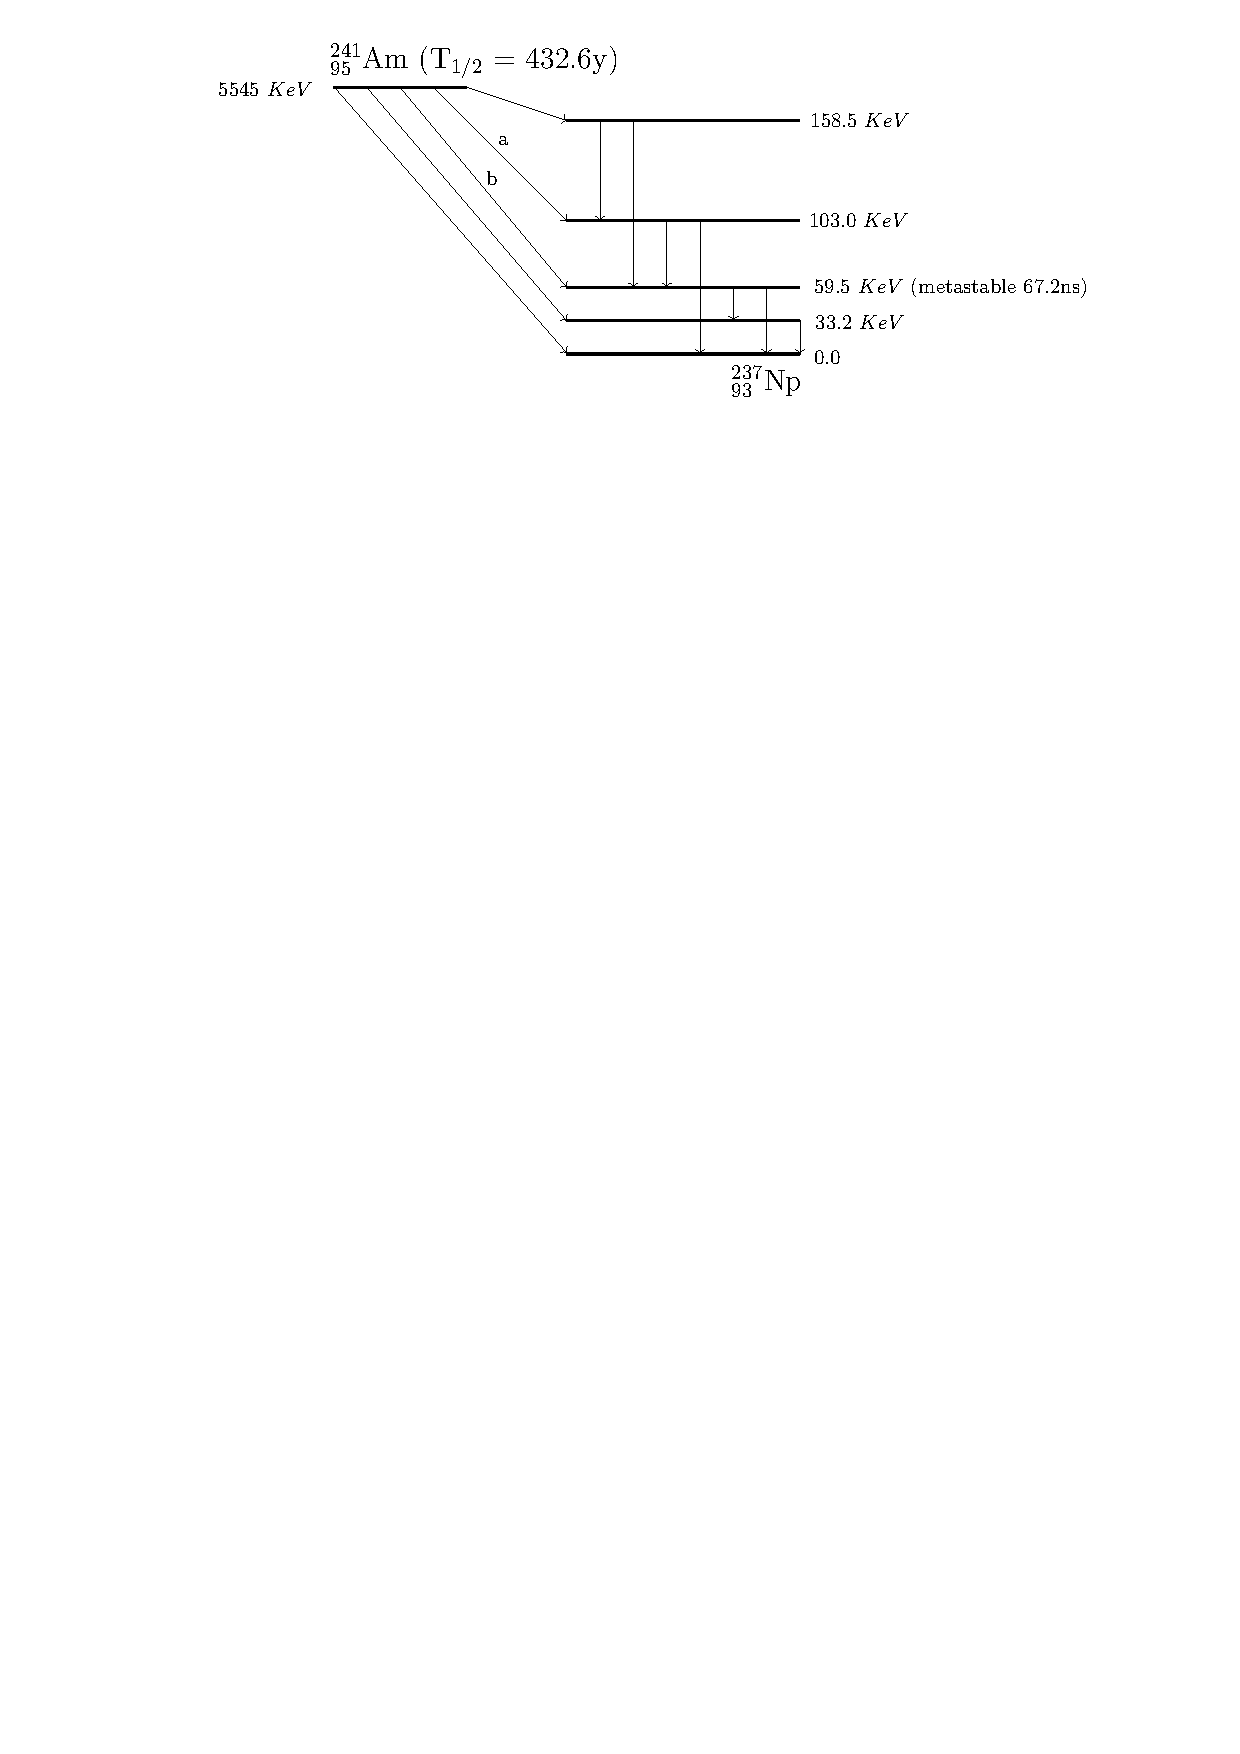
\includegraphics[width=\columnwidth]{images/decay.pdf}
	\caption{Decay scheme, showing the many $\alpha$ decays
    and the associated nuclear isomers of Np}
    \label{decay}
\end{figure}
Out of the energies, we will be seeing only the transitions
that are the most possible, which, for us here, is what I
have labelled \texttt{a} and \texttt{b}. `b' holds the crown
for the most probable $\alpha$ transition with the
probability of 84.8\% and then comes 'a' with the
probability of 13.1\%. Each one of the alpha particle
ejected makes a different (out of the 4) nuclear isomer. One
of them, associated with the `b' transition, makes the most
stable isomer. We call it \emph{metastable}, as its halflife is in
the order of ns, instead of \emph{prompt} isomers, which
stay back in the order of ps. which others are. Most of what
we see in gamma energy comes to this energy level, stays
there for a while, and then decays with a half-life of
$67.2$ ns

\subsection{Setup}
We use a setup where we use a NaI scintillation detector for
gamma detection, and a solid state photodiode for the alpha
detection. We pass them separately through amplifiers and
then pass it to our dual channel MCA.

For the $\alpha$ readings, we pass it through a
preamplifier, that inverts the signal and sends it over to
two daisy chained amplifiers. They are so, because we didn't
have enough amplification to bring up the voltage of the
alpha signals. 

\begin{figure}[H]
    \centering
    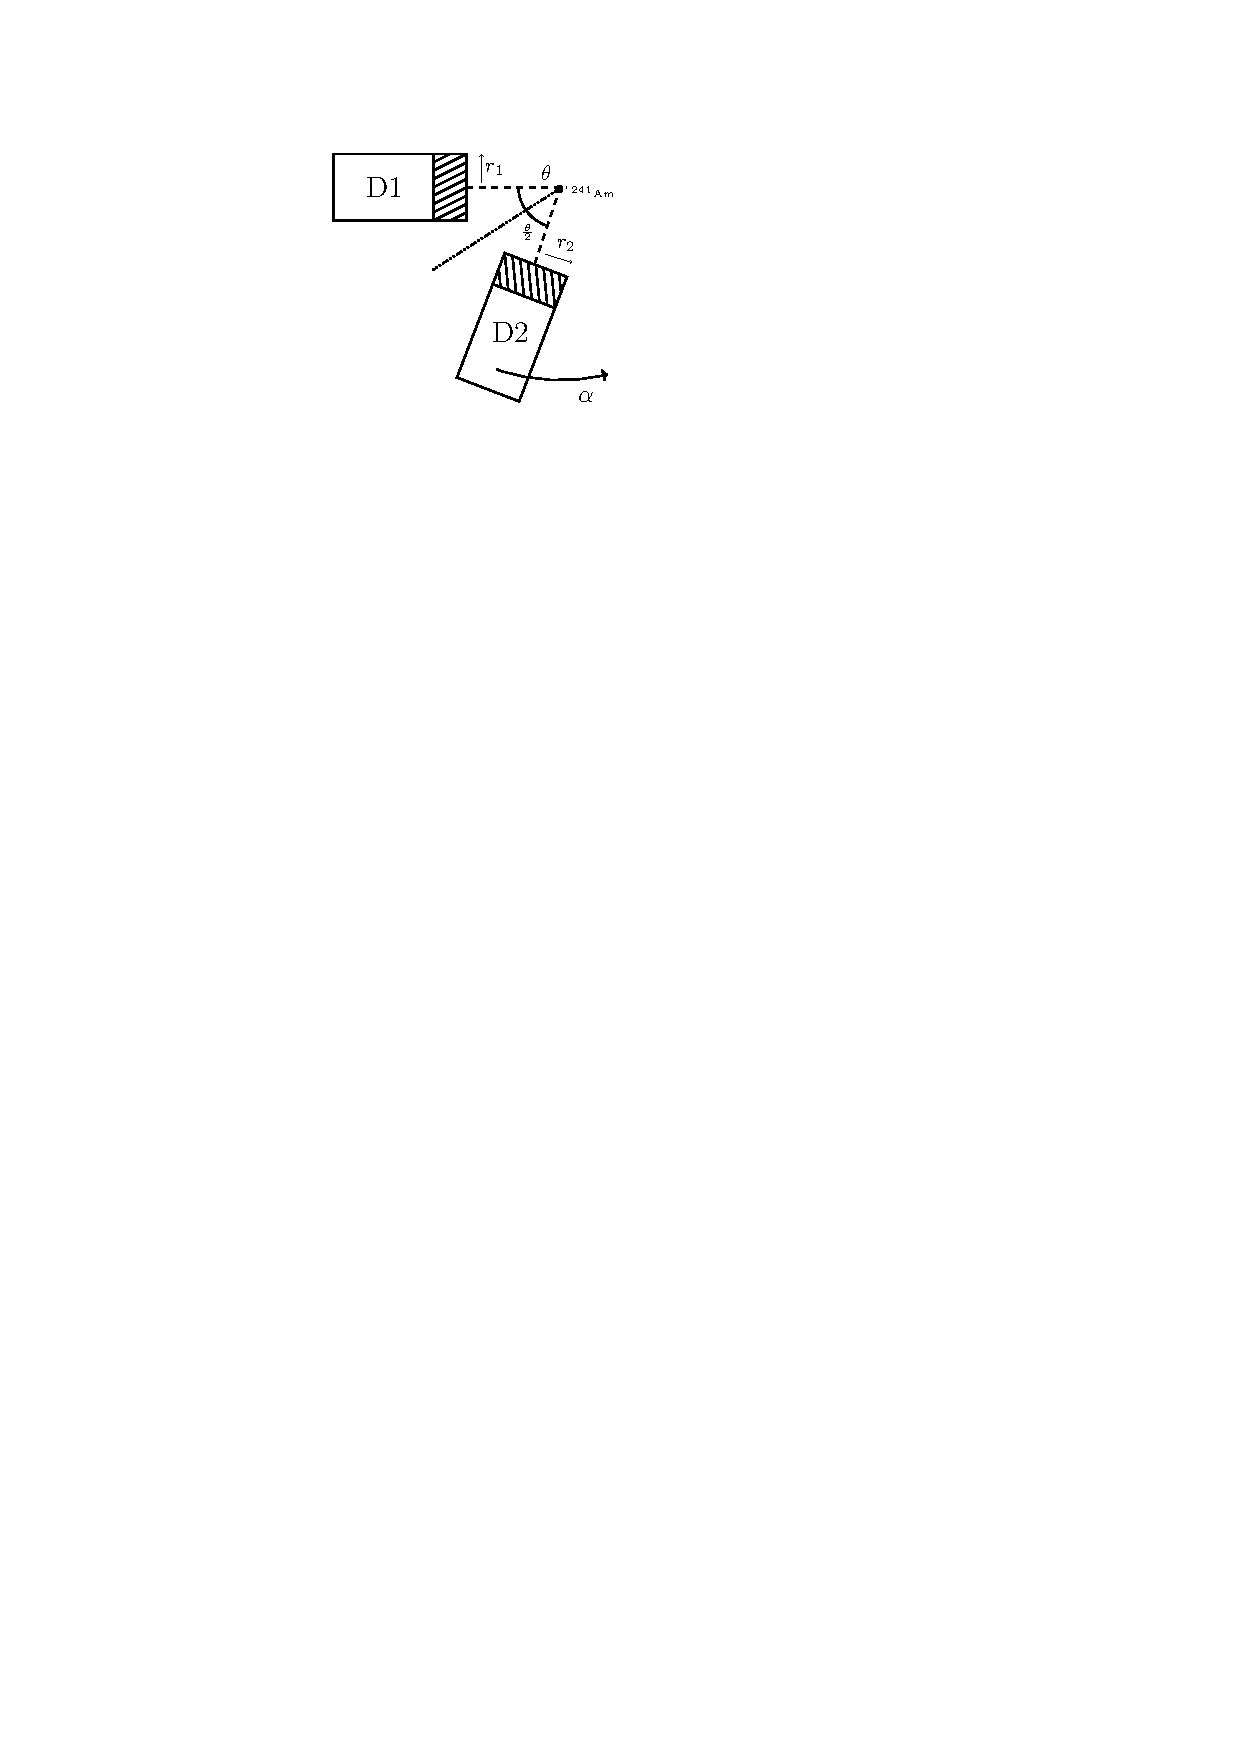
\includegraphics[width=0.6\columnwidth]{images/detectors.pdf}
    \caption{The most general detector setup}
    \label{detect}
\end{figure}

Here in this diagram, I have represented a very simplified
view of two detectors facing a source, and I want to
calculate the coicidence counts for different relative
angles. One of the detectors, $D1$, is fixed, and the other
moves around. The angles that I will be mentioning have been
mentioned in the figure itself. 

We will start by calculating the angles $\beta$. For any
given detector, say $D1$, I can say that:
\begin{align}
   tan \beta_1 = \frac{r_1}{d_1}
\end{align}
\noindent Where $r_1$ is the radius of the face of the detector and
$d_1$ is the distance of the face from the source. Similary,
for the second detector, we can say:
\begin{align}
   tan \beta_2 = \frac{r_2}{d_2}
\end{align}

\noindent The counting rate ($s^{-1}$) for any detector can
be given by:
\begin{equation}
    N = A\epsilon \frac{\Omega}{4\pi}
\end{equation}
\noindent Where $A$ is the number of gamma rays emitted by
the radioactive source, $\epsilon$ is the efficiency of the
detector, and $\frac{\Omega}{4\pi}$ is the fraction of the
solid angle subtended by the detector face on the point
source (for our purposes now). This ratio is also called the
\emph{geometrical efficiency} of the detector. Of course
here, the `spherical cap', as we call the subtended small
cap from the detector face, has an area of $2\pi
R^2(1-cos\beta)$. We get that using a very simple integral:
\begin{align}
    I &= R^2 \int_{\phi = 0}^{2\pi} d\phi \int _{cos \beta}^{1}
    d(cos\theta) \nonumber\\
    &= 2\pi R^2 (1 - cos\beta)
\end{align}
\noindent Now we can say here that our efficiency comes down
to:
\begin{equation}
    \frac{\Omega}{4\pi} = \frac{1}{2}(1-cos\beta)
\end{equation}
\noindent Typically, the values of $\beta$ are small. Which
means that the radius of the detector is small, compared to
the distance from the source. Smaller values mean a smaller
geometrical efficiency, but a higher angular resolution.

Consider here, that we have two rays, one alpha, and one
gamma ray being emitted from the source. We are assuming
that $\alpha$ is detected by $D1$ and $\gamma$ by $D2$. Now
these can be either \emph{correlated} or
\emph{uncorrelated}. If both the detections occur within a
small delay window, they are said to be \emph{temporally
coincident}. The relative probability that the gamma will be
emitted at an angle $\theta$ w.r.t the $\alpha$ is given by
$W(\theta)$, and it's called the angular distribution. Given
that nuclear spins and energy conservation comes to play
here, the angles will be relative to the underlying physics
in play here. I could not go into much detail here, and I
will leave the function at $W(\theta)$ now. 

Circling back, we come to the two detector setup again.
Here, I have, the counting rates as:

\begin{align}
    N_1 &= A\epsilon_1 \frac{\Omega_1}{4\pi} \nonumber\\
    N_2 &= A\epsilon_2 \frac{\Omega_2}{4\pi}
\end{align}

If the rays are uncorrelated, the 'true' coincidences will
be given by:

\begin{equation}
    C_\nu = A \epsilon_1 \epsilon_2 \ \frac{\Omega_2}{4\pi}
    \frac{\Omega_2}{4\pi}
\end{equation}

We are assuming that at the angle that we are keeping the
detectors, we will catch correlated rays. For a given angle,
we will have a critical angle and an overlap between the
spherical caps. The overlap, which we call $\Delta \Omega$,
is what we are looking for. Because then, for correlated
events, we will have:
\begin{equation}
    C_C = A \epsilon_1 \epsilon_2 \frac{\Delta \Omega}{4 \pi}
\end{equation}

This calculation has been done with the help of Filipe et
al, and with a small addition, we can notice how his method
can be extended to include all angles. We will go on a small
geometric digression here.

For making the problem a bit simpler, we take note of the
fact that no matter what angle the particles are emitted, we
will have the same form of equations. To understand this a
bit better, we conduct a thought experiment. The
$\frac{\Delta \Omega}{4\pi}$ is proportional to the
difference in the area of the immovable detector and the
\emph{ghost area} of the movable detector. We can understand
this as if we have a mirror at an angle dependent on the
angle between the consecutive correlated emissions. So if we
have a alpha, and then a gamma being let out with a relative
angle of $\theta$, then we will have a mirror at an angle of
$\frac{\pi}{2} - \frac{\theta}{2}$, facing the alpha detector. This
can be understood better by looking at the diagram in
figure \ref{detect}. Essentially, if we have both of the detectors at a
relative angle of $\theta$, their sperical caps will match
perfectly, thus showing us that that angle is the one we
will see maximum coincidence counts at.

After that, we can see that at any other angle, we will have
the exact same situation. The angle $\alpha$ that we take as
the amount of rotation for $D2$, is only taken from the
proper axis, that is at $\theta$ from the $D1$ detector.
With that in mind, we will go forward and set the angle here
to be $\pi$, as that makes it easier for us to imagine
scenarios. Further, just to make everyone's life simpler,
and also because of the fact that we do not have any actual
measurements for this part, I am making them be at the same
distances from the source, and allowing them to have the
same $\beta$. 

\begin{figure}[H]
    \centering
    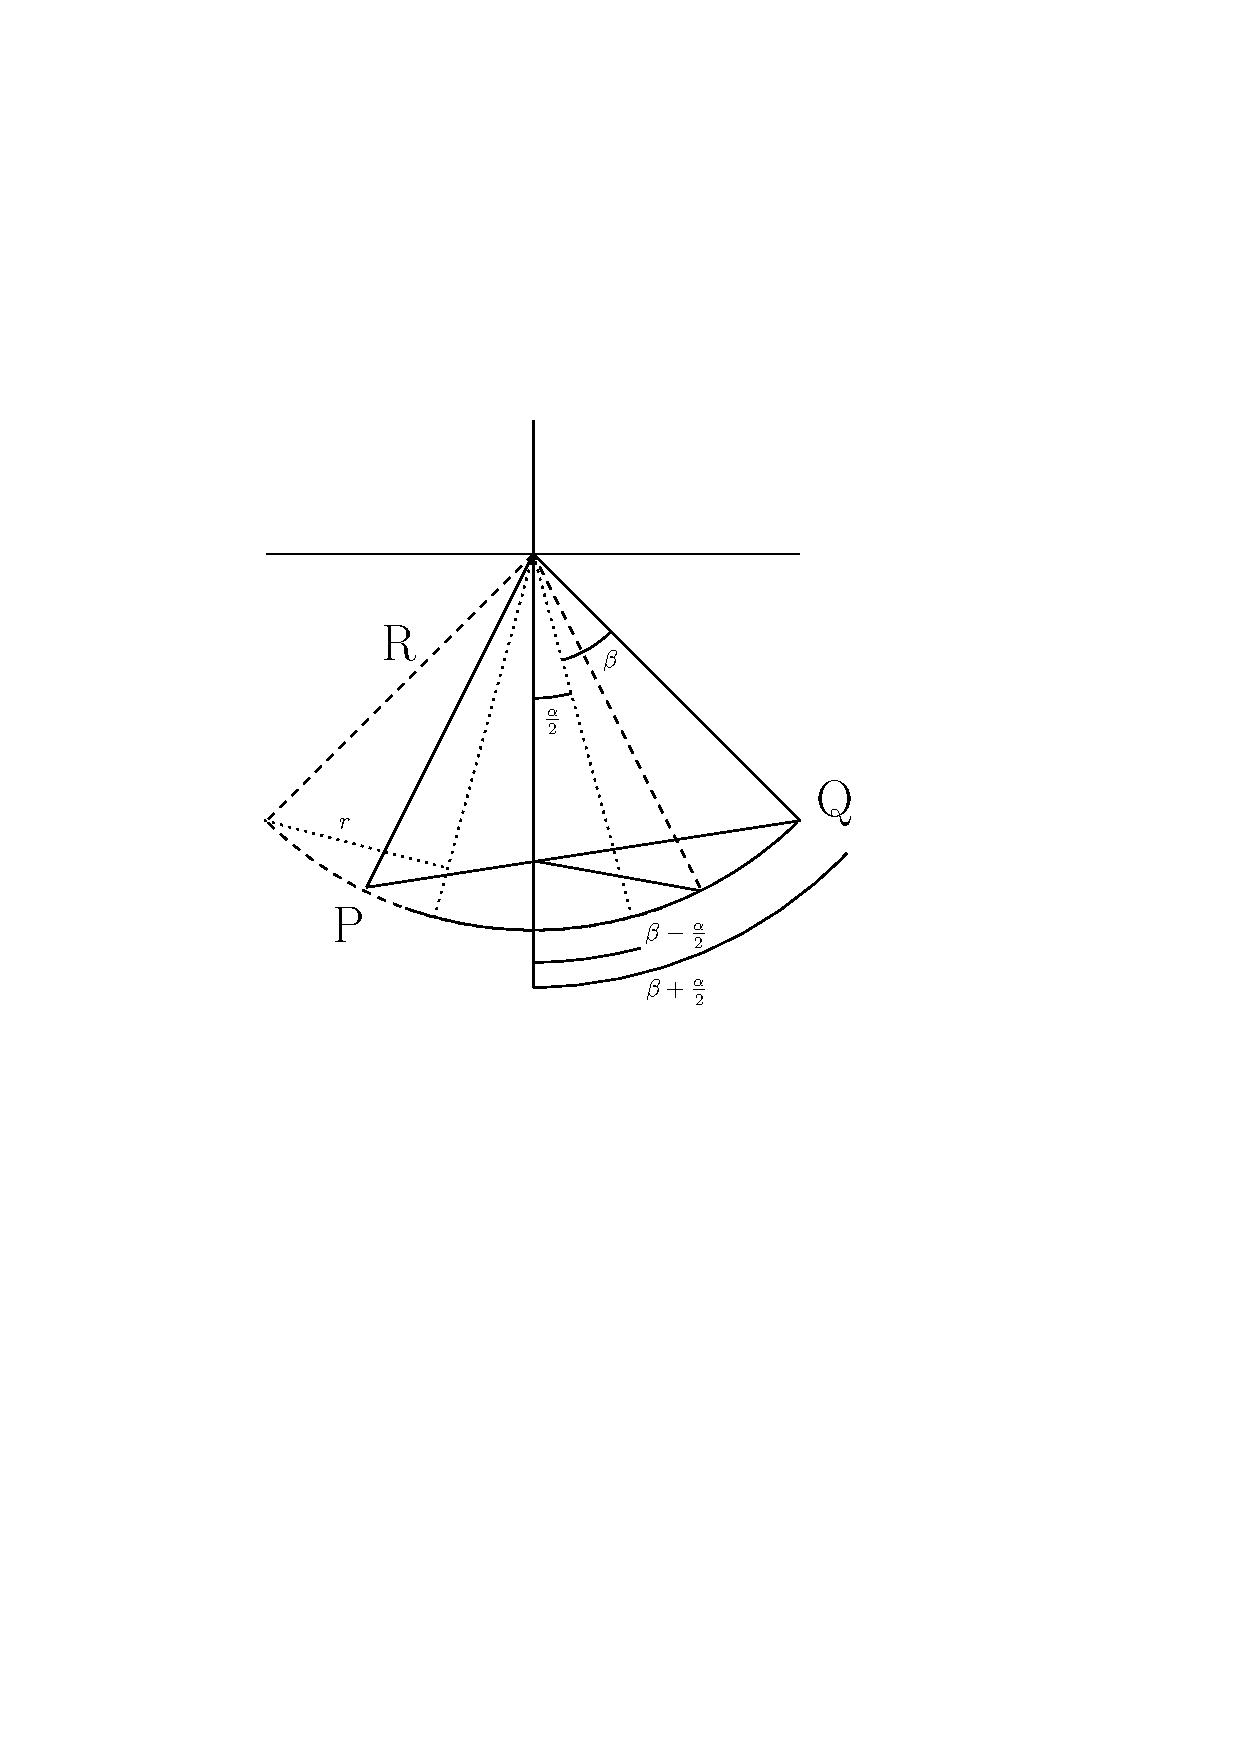
\includegraphics[width=0.6\columnwidth]{images/diag.pdf}
    \caption{Detectors in XY plane}
    \label{diag}
\end{figure}

With that in mind, we can define our coordinate system and
place the center of the face of the fixed detector at
$(d\sin(\alpha/2), -d\cos(\alpha/2), 0)$ and the movable
detector at $(d\sin(\alpha/2), d\cos(\alpha/2), 0)$. That will
make the reflection to come at $(-d\sin(\alpha/2),
-d\cos(\alpha/2), 0)$.

Once we have the coordinates, calculating P and Q in the
graph is a piece of cake. We have:
\begin{align}
    P &= (-R(\beta-\frac{\alpha}{2}),
    -R\cos(\beta-\frac{\alpha}{2}), 0) \\
    R &= (R(\beta+\frac{\alpha}{2}),
    -R\cos(\beta+\frac{\alpha}{2}), 0)
\end{align}
\noindent The equation of the plane perpindicular to the XY
plane will be given by:
\begin{equation}
    y =
    \tan(\frac{\alpha}{2})(x+R\sin(\beta-\frac{\alpha}{2})) -
    R\cos(\beta-\frac{\alpha}{2})
\end{equation}

We wish to compute the intersection of the two spherical
caps, which as you would imagine, can be divided into
quadrants and will have the same area in all four of those.
If we pick one of the quadrants, we will have:

\begin{align}
    -\sqrt{R^2-x^2} \leq y &\leq
    \tan(\frac{\alpha}{2})(x+R\sin(\beta-\frac{\alpha}{2}))
    \nonumber\\
    &- R\cos(\beta-\frac{\alpha}{2}) \\
    - R\sin(\beta-\frac{\alpha}{2}) \leq x &\leq 0
\end{align}

We can then proceed to calculate the area using the usual
surface integral, with the small area:
\begin{equation}
    ds = \frac{R}{\sqrt{R^2-x^2-y^2}}
\end{equation}

The area is then given by (with R set to be 1), as we need
the solid angle $\Delta \Omega$ given by:
\begin{equation}
    4\int_{-\sin(\beta-\frac{\alpha}{2})}^{0}
    \int_{-sqrt{1-x^2}}^{\tan(\frac{\alpha}{2})(x+\sin(\beta -
    \frac{\alpha}{2}) - \cos(\beta -\frac{\alpha}{2}))}
    \frac{1}{\sqrt{1-x^2-y^2}} dy dx
\end{equation}

On integrating the equation above, we get a very complicated
solution:
\begin{align}
    4(\arccot&\left(\frac{\sqrt{2}\sin\frac{\left|\alpha\right|}{2}}{\sqrt{\cos\alpha-\cos2\beta}}\right)
    \nonumber \\&-\arccot\left(\frac{\sqrt{2}\cos\beta\sin\frac{\left|\alpha\right|}{2}}{\sqrt{\cos\alpha-\cos2\beta}}\right)
    \cos\beta)
    \label{eq:delom}
\end{align}

We see that we get for a given value of $\beta$, we obtain a
periodic function of $\alpha$, with a period of $2\pi$. In
the neighbourhood of $\alpha=0$, we see that the function is
positive and defined only for $\alpha \leq 2\beta$. At
$2\beta$, the function vanishes, which turns out to be our
critical angle. When we take $\beta \rightarrow 0$, we have
the highest angular resolution, and the rate of coincidences
matches the angular distribution function.

For our case, if we are assuming that we have a distribution
of $\theta$, instead of a solid single value, we will have
the same expression for every angle. The difference there,
will be that $\alpha \rightarrow \alpha_\theta$, where
$\theta$ is the relative angle between the particles. Then,
we will have someting like:

\begin{equation}
    \boxed{
        C_C = \int^{\theta} A\epsilon_1\epsilon_2 W(\theta) \frac{\Delta
        \Omega(\alpha_\theta, \beta)}{4\pi}
    }
\end{equation}

\section{Experiment}
For the scope of this experiment, we couldn't go very far,
but we were able to `prove' coincidence using a coincidence
heatmap. According to the theory that we have, within a
short interval of time, the maximum coincidence should occur
with the $5485.56$KeV $\alpha$ and the $59.5$KeV $\gamma$.
So logically, we should get the coincidence heatmap with the
peak at the intersection of these two energies, which we
did, and presented ahead.

\subsection{Hardware}
For the preamplification, amplification, and detection of
the alpha particle, we used the whole of PHYWE's Rutherford
experiment setup, complete with a vacuum pump and monitor.
Our only option here was to keep the sample at a
$45^{\circ}$ angle, because the sample could only fire one
way, and equal angles from both the detectors seemed the
best choice to go with. Similarly for the gamma detection,
we went with a normal NaI scintillation and SCA setup, only
using the shaping and amplification module on the equipment. 

For consolidating the two signals and as the MCA, we used
CSpark's dual input MCA, which could do $500ns$ resolution
for the coincidence. So if we had a coincidence measurement
within $500ns$, both the outputs will be high in the log.
All of our graphs have been sourced from this machine, with
their code and some of our addition.

\subsection{Spectra}
\subsubsection{Alpha}
We can clearly identify two peaks here, those two peaks have
been used to callibrate the scale for all alpha channels
here, and in the heatmap. We had some noise, and the
amplification wasn't enough, which caused the coincidence
counts to be a bit less than expected. a higher
amplification would lift actual measurements off of the mud
and make the coincidence a bit more evident.
\begin{figure}[H]
	\centering
	\resizebox{0.8\columnwidth}{!}{%
		%% Creator: Matplotlib, PGF backend
%%
%% To include the figure in your LaTeX document, write
%%   \input{<filename>.pgf}
%%
%% Make sure the required packages are loaded in your preamble
%%   \usepackage{pgf}
%%
%% Figures using additional raster images can only be included by \input if
%% they are in the same directory as the main LaTeX file. For loading figures
%% from other directories you can use the `import` package
%%   \usepackage{import}
%%
%% and then include the figures with
%%   \import{<path to file>}{<filename>.pgf}
%%
%% Matplotlib used the following preamble
%%   \usepackage{fontspec}
%%   \setmainfont{DejaVuSerif.ttf}[Path=\detokenize{/home/spandan/.local/lib/python3.9/site-packages/matplotlib/mpl-data/fonts/ttf/}]
%%   \setsansfont{DejaVuSans.ttf}[Path=\detokenize{/home/spandan/.local/lib/python3.9/site-packages/matplotlib/mpl-data/fonts/ttf/}]
%%   \setmonofont{DejaVuSansMono.ttf}[Path=\detokenize{/home/spandan/.local/lib/python3.9/site-packages/matplotlib/mpl-data/fonts/ttf/}]
%%
\begingroup%
\makeatletter%
\begin{pgfpicture}%
\pgfpathrectangle{\pgfpointorigin}{\pgfqpoint{10.000000in}{10.000000in}}%
\pgfusepath{use as bounding box, clip}%
\begin{pgfscope}%
\pgfsetbuttcap%
\pgfsetmiterjoin%
\pgfsetlinewidth{0.000000pt}%
\definecolor{currentstroke}{rgb}{1.000000,1.000000,1.000000}%
\pgfsetstrokecolor{currentstroke}%
\pgfsetstrokeopacity{0.000000}%
\pgfsetdash{}{0pt}%
\pgfpathmoveto{\pgfqpoint{0.000000in}{0.000000in}}%
\pgfpathlineto{\pgfqpoint{10.000000in}{0.000000in}}%
\pgfpathlineto{\pgfqpoint{10.000000in}{10.000000in}}%
\pgfpathlineto{\pgfqpoint{0.000000in}{10.000000in}}%
\pgfpathclose%
\pgfusepath{}%
\end{pgfscope}%
\begin{pgfscope}%
\pgfsetbuttcap%
\pgfsetmiterjoin%
\definecolor{currentfill}{rgb}{1.000000,1.000000,1.000000}%
\pgfsetfillcolor{currentfill}%
\pgfsetlinewidth{0.000000pt}%
\definecolor{currentstroke}{rgb}{0.000000,0.000000,0.000000}%
\pgfsetstrokecolor{currentstroke}%
\pgfsetstrokeopacity{0.000000}%
\pgfsetdash{}{0pt}%
\pgfpathmoveto{\pgfqpoint{1.250000in}{1.250000in}}%
\pgfpathlineto{\pgfqpoint{9.000000in}{1.250000in}}%
\pgfpathlineto{\pgfqpoint{9.000000in}{8.800000in}}%
\pgfpathlineto{\pgfqpoint{1.250000in}{8.800000in}}%
\pgfpathclose%
\pgfusepath{fill}%
\end{pgfscope}%
\begin{pgfscope}%
\pgfsetbuttcap%
\pgfsetroundjoin%
\definecolor{currentfill}{rgb}{0.000000,0.000000,0.000000}%
\pgfsetfillcolor{currentfill}%
\pgfsetlinewidth{0.803000pt}%
\definecolor{currentstroke}{rgb}{0.000000,0.000000,0.000000}%
\pgfsetstrokecolor{currentstroke}%
\pgfsetdash{}{0pt}%
\pgfsys@defobject{currentmarker}{\pgfqpoint{0.000000in}{-0.048611in}}{\pgfqpoint{0.000000in}{0.000000in}}{%
\pgfpathmoveto{\pgfqpoint{0.000000in}{0.000000in}}%
\pgfpathlineto{\pgfqpoint{0.000000in}{-0.048611in}}%
\pgfusepath{stroke,fill}%
}%
\begin{pgfscope}%
\pgfsys@transformshift{2.079330in}{1.250000in}%
\pgfsys@useobject{currentmarker}{}%
\end{pgfscope}%
\end{pgfscope}%
\begin{pgfscope}%
\definecolor{textcolor}{rgb}{0.000000,0.000000,0.000000}%
\pgfsetstrokecolor{textcolor}%
\pgfsetfillcolor{textcolor}%
\pgftext[x=2.079330in,y=1.152778in,,top]{\color{textcolor}\sffamily\fontsize{10.000000}{12.000000}\selectfont \(\displaystyle {5400}\)}%
\end{pgfscope}%
\begin{pgfscope}%
\pgfsetbuttcap%
\pgfsetroundjoin%
\definecolor{currentfill}{rgb}{0.000000,0.000000,0.000000}%
\pgfsetfillcolor{currentfill}%
\pgfsetlinewidth{0.803000pt}%
\definecolor{currentstroke}{rgb}{0.000000,0.000000,0.000000}%
\pgfsetstrokecolor{currentstroke}%
\pgfsetdash{}{0pt}%
\pgfsys@defobject{currentmarker}{\pgfqpoint{0.000000in}{-0.048611in}}{\pgfqpoint{0.000000in}{0.000000in}}{%
\pgfpathmoveto{\pgfqpoint{0.000000in}{0.000000in}}%
\pgfpathlineto{\pgfqpoint{0.000000in}{-0.048611in}}%
\pgfusepath{stroke,fill}%
}%
\begin{pgfscope}%
\pgfsys@transformshift{3.452472in}{1.250000in}%
\pgfsys@useobject{currentmarker}{}%
\end{pgfscope}%
\end{pgfscope}%
\begin{pgfscope}%
\definecolor{textcolor}{rgb}{0.000000,0.000000,0.000000}%
\pgfsetstrokecolor{textcolor}%
\pgfsetfillcolor{textcolor}%
\pgftext[x=3.452472in,y=1.152778in,,top]{\color{textcolor}\sffamily\fontsize{10.000000}{12.000000}\selectfont \(\displaystyle {5500}\)}%
\end{pgfscope}%
\begin{pgfscope}%
\pgfsetbuttcap%
\pgfsetroundjoin%
\definecolor{currentfill}{rgb}{0.000000,0.000000,0.000000}%
\pgfsetfillcolor{currentfill}%
\pgfsetlinewidth{0.803000pt}%
\definecolor{currentstroke}{rgb}{0.000000,0.000000,0.000000}%
\pgfsetstrokecolor{currentstroke}%
\pgfsetdash{}{0pt}%
\pgfsys@defobject{currentmarker}{\pgfqpoint{0.000000in}{-0.048611in}}{\pgfqpoint{0.000000in}{0.000000in}}{%
\pgfpathmoveto{\pgfqpoint{0.000000in}{0.000000in}}%
\pgfpathlineto{\pgfqpoint{0.000000in}{-0.048611in}}%
\pgfusepath{stroke,fill}%
}%
\begin{pgfscope}%
\pgfsys@transformshift{4.825614in}{1.250000in}%
\pgfsys@useobject{currentmarker}{}%
\end{pgfscope}%
\end{pgfscope}%
\begin{pgfscope}%
\definecolor{textcolor}{rgb}{0.000000,0.000000,0.000000}%
\pgfsetstrokecolor{textcolor}%
\pgfsetfillcolor{textcolor}%
\pgftext[x=4.825614in,y=1.152778in,,top]{\color{textcolor}\sffamily\fontsize{10.000000}{12.000000}\selectfont \(\displaystyle {5600}\)}%
\end{pgfscope}%
\begin{pgfscope}%
\pgfsetbuttcap%
\pgfsetroundjoin%
\definecolor{currentfill}{rgb}{0.000000,0.000000,0.000000}%
\pgfsetfillcolor{currentfill}%
\pgfsetlinewidth{0.803000pt}%
\definecolor{currentstroke}{rgb}{0.000000,0.000000,0.000000}%
\pgfsetstrokecolor{currentstroke}%
\pgfsetdash{}{0pt}%
\pgfsys@defobject{currentmarker}{\pgfqpoint{0.000000in}{-0.048611in}}{\pgfqpoint{0.000000in}{0.000000in}}{%
\pgfpathmoveto{\pgfqpoint{0.000000in}{0.000000in}}%
\pgfpathlineto{\pgfqpoint{0.000000in}{-0.048611in}}%
\pgfusepath{stroke,fill}%
}%
\begin{pgfscope}%
\pgfsys@transformshift{6.198756in}{1.250000in}%
\pgfsys@useobject{currentmarker}{}%
\end{pgfscope}%
\end{pgfscope}%
\begin{pgfscope}%
\definecolor{textcolor}{rgb}{0.000000,0.000000,0.000000}%
\pgfsetstrokecolor{textcolor}%
\pgfsetfillcolor{textcolor}%
\pgftext[x=6.198756in,y=1.152778in,,top]{\color{textcolor}\sffamily\fontsize{10.000000}{12.000000}\selectfont \(\displaystyle {5700}\)}%
\end{pgfscope}%
\begin{pgfscope}%
\pgfsetbuttcap%
\pgfsetroundjoin%
\definecolor{currentfill}{rgb}{0.000000,0.000000,0.000000}%
\pgfsetfillcolor{currentfill}%
\pgfsetlinewidth{0.803000pt}%
\definecolor{currentstroke}{rgb}{0.000000,0.000000,0.000000}%
\pgfsetstrokecolor{currentstroke}%
\pgfsetdash{}{0pt}%
\pgfsys@defobject{currentmarker}{\pgfqpoint{0.000000in}{-0.048611in}}{\pgfqpoint{0.000000in}{0.000000in}}{%
\pgfpathmoveto{\pgfqpoint{0.000000in}{0.000000in}}%
\pgfpathlineto{\pgfqpoint{0.000000in}{-0.048611in}}%
\pgfusepath{stroke,fill}%
}%
\begin{pgfscope}%
\pgfsys@transformshift{7.571898in}{1.250000in}%
\pgfsys@useobject{currentmarker}{}%
\end{pgfscope}%
\end{pgfscope}%
\begin{pgfscope}%
\definecolor{textcolor}{rgb}{0.000000,0.000000,0.000000}%
\pgfsetstrokecolor{textcolor}%
\pgfsetfillcolor{textcolor}%
\pgftext[x=7.571898in,y=1.152778in,,top]{\color{textcolor}\sffamily\fontsize{10.000000}{12.000000}\selectfont \(\displaystyle {5800}\)}%
\end{pgfscope}%
\begin{pgfscope}%
\pgfsetbuttcap%
\pgfsetroundjoin%
\definecolor{currentfill}{rgb}{0.000000,0.000000,0.000000}%
\pgfsetfillcolor{currentfill}%
\pgfsetlinewidth{0.803000pt}%
\definecolor{currentstroke}{rgb}{0.000000,0.000000,0.000000}%
\pgfsetstrokecolor{currentstroke}%
\pgfsetdash{}{0pt}%
\pgfsys@defobject{currentmarker}{\pgfqpoint{0.000000in}{-0.048611in}}{\pgfqpoint{0.000000in}{0.000000in}}{%
\pgfpathmoveto{\pgfqpoint{0.000000in}{0.000000in}}%
\pgfpathlineto{\pgfqpoint{0.000000in}{-0.048611in}}%
\pgfusepath{stroke,fill}%
}%
\begin{pgfscope}%
\pgfsys@transformshift{8.945040in}{1.250000in}%
\pgfsys@useobject{currentmarker}{}%
\end{pgfscope}%
\end{pgfscope}%
\begin{pgfscope}%
\definecolor{textcolor}{rgb}{0.000000,0.000000,0.000000}%
\pgfsetstrokecolor{textcolor}%
\pgfsetfillcolor{textcolor}%
\pgftext[x=8.945040in,y=1.152778in,,top]{\color{textcolor}\sffamily\fontsize{10.000000}{12.000000}\selectfont \(\displaystyle {5900}\)}%
\end{pgfscope}%
\begin{pgfscope}%
\definecolor{textcolor}{rgb}{0.000000,0.000000,0.000000}%
\pgfsetstrokecolor{textcolor}%
\pgfsetfillcolor{textcolor}%
\pgftext[x=5.125000in,y=0.962809in,,top]{\color{textcolor}\sffamily\fontsize{10.000000}{12.000000}\selectfont Energy (KeV)}%
\end{pgfscope}%
\begin{pgfscope}%
\pgfsetbuttcap%
\pgfsetroundjoin%
\definecolor{currentfill}{rgb}{0.000000,0.000000,0.000000}%
\pgfsetfillcolor{currentfill}%
\pgfsetlinewidth{0.803000pt}%
\definecolor{currentstroke}{rgb}{0.000000,0.000000,0.000000}%
\pgfsetstrokecolor{currentstroke}%
\pgfsetdash{}{0pt}%
\pgfsys@defobject{currentmarker}{\pgfqpoint{-0.048611in}{0.000000in}}{\pgfqpoint{-0.000000in}{0.000000in}}{%
\pgfpathmoveto{\pgfqpoint{-0.000000in}{0.000000in}}%
\pgfpathlineto{\pgfqpoint{-0.048611in}{0.000000in}}%
\pgfusepath{stroke,fill}%
}%
\begin{pgfscope}%
\pgfsys@transformshift{1.250000in}{1.596208in}%
\pgfsys@useobject{currentmarker}{}%
\end{pgfscope}%
\end{pgfscope}%
\begin{pgfscope}%
\definecolor{textcolor}{rgb}{0.000000,0.000000,0.000000}%
\pgfsetstrokecolor{textcolor}%
\pgfsetfillcolor{textcolor}%
\pgftext[x=1.083333in, y=1.543446in, left, base]{\color{textcolor}\sffamily\fontsize{10.000000}{12.000000}\selectfont \(\displaystyle {0}\)}%
\end{pgfscope}%
\begin{pgfscope}%
\pgfsetbuttcap%
\pgfsetroundjoin%
\definecolor{currentfill}{rgb}{0.000000,0.000000,0.000000}%
\pgfsetfillcolor{currentfill}%
\pgfsetlinewidth{0.803000pt}%
\definecolor{currentstroke}{rgb}{0.000000,0.000000,0.000000}%
\pgfsetstrokecolor{currentstroke}%
\pgfsetdash{}{0pt}%
\pgfsys@defobject{currentmarker}{\pgfqpoint{-0.048611in}{0.000000in}}{\pgfqpoint{-0.000000in}{0.000000in}}{%
\pgfpathmoveto{\pgfqpoint{-0.000000in}{0.000000in}}%
\pgfpathlineto{\pgfqpoint{-0.048611in}{0.000000in}}%
\pgfusepath{stroke,fill}%
}%
\begin{pgfscope}%
\pgfsys@transformshift{1.250000in}{2.557481in}%
\pgfsys@useobject{currentmarker}{}%
\end{pgfscope}%
\end{pgfscope}%
\begin{pgfscope}%
\definecolor{textcolor}{rgb}{0.000000,0.000000,0.000000}%
\pgfsetstrokecolor{textcolor}%
\pgfsetfillcolor{textcolor}%
\pgftext[x=0.874999in, y=2.504720in, left, base]{\color{textcolor}\sffamily\fontsize{10.000000}{12.000000}\selectfont \(\displaystyle {1000}\)}%
\end{pgfscope}%
\begin{pgfscope}%
\pgfsetbuttcap%
\pgfsetroundjoin%
\definecolor{currentfill}{rgb}{0.000000,0.000000,0.000000}%
\pgfsetfillcolor{currentfill}%
\pgfsetlinewidth{0.803000pt}%
\definecolor{currentstroke}{rgb}{0.000000,0.000000,0.000000}%
\pgfsetstrokecolor{currentstroke}%
\pgfsetdash{}{0pt}%
\pgfsys@defobject{currentmarker}{\pgfqpoint{-0.048611in}{0.000000in}}{\pgfqpoint{-0.000000in}{0.000000in}}{%
\pgfpathmoveto{\pgfqpoint{-0.000000in}{0.000000in}}%
\pgfpathlineto{\pgfqpoint{-0.048611in}{0.000000in}}%
\pgfusepath{stroke,fill}%
}%
\begin{pgfscope}%
\pgfsys@transformshift{1.250000in}{3.518755in}%
\pgfsys@useobject{currentmarker}{}%
\end{pgfscope}%
\end{pgfscope}%
\begin{pgfscope}%
\definecolor{textcolor}{rgb}{0.000000,0.000000,0.000000}%
\pgfsetstrokecolor{textcolor}%
\pgfsetfillcolor{textcolor}%
\pgftext[x=0.874999in, y=3.465994in, left, base]{\color{textcolor}\sffamily\fontsize{10.000000}{12.000000}\selectfont \(\displaystyle {2000}\)}%
\end{pgfscope}%
\begin{pgfscope}%
\pgfsetbuttcap%
\pgfsetroundjoin%
\definecolor{currentfill}{rgb}{0.000000,0.000000,0.000000}%
\pgfsetfillcolor{currentfill}%
\pgfsetlinewidth{0.803000pt}%
\definecolor{currentstroke}{rgb}{0.000000,0.000000,0.000000}%
\pgfsetstrokecolor{currentstroke}%
\pgfsetdash{}{0pt}%
\pgfsys@defobject{currentmarker}{\pgfqpoint{-0.048611in}{0.000000in}}{\pgfqpoint{-0.000000in}{0.000000in}}{%
\pgfpathmoveto{\pgfqpoint{-0.000000in}{0.000000in}}%
\pgfpathlineto{\pgfqpoint{-0.048611in}{0.000000in}}%
\pgfusepath{stroke,fill}%
}%
\begin{pgfscope}%
\pgfsys@transformshift{1.250000in}{4.480029in}%
\pgfsys@useobject{currentmarker}{}%
\end{pgfscope}%
\end{pgfscope}%
\begin{pgfscope}%
\definecolor{textcolor}{rgb}{0.000000,0.000000,0.000000}%
\pgfsetstrokecolor{textcolor}%
\pgfsetfillcolor{textcolor}%
\pgftext[x=0.874999in, y=4.427267in, left, base]{\color{textcolor}\sffamily\fontsize{10.000000}{12.000000}\selectfont \(\displaystyle {3000}\)}%
\end{pgfscope}%
\begin{pgfscope}%
\pgfsetbuttcap%
\pgfsetroundjoin%
\definecolor{currentfill}{rgb}{0.000000,0.000000,0.000000}%
\pgfsetfillcolor{currentfill}%
\pgfsetlinewidth{0.803000pt}%
\definecolor{currentstroke}{rgb}{0.000000,0.000000,0.000000}%
\pgfsetstrokecolor{currentstroke}%
\pgfsetdash{}{0pt}%
\pgfsys@defobject{currentmarker}{\pgfqpoint{-0.048611in}{0.000000in}}{\pgfqpoint{-0.000000in}{0.000000in}}{%
\pgfpathmoveto{\pgfqpoint{-0.000000in}{0.000000in}}%
\pgfpathlineto{\pgfqpoint{-0.048611in}{0.000000in}}%
\pgfusepath{stroke,fill}%
}%
\begin{pgfscope}%
\pgfsys@transformshift{1.250000in}{5.441303in}%
\pgfsys@useobject{currentmarker}{}%
\end{pgfscope}%
\end{pgfscope}%
\begin{pgfscope}%
\definecolor{textcolor}{rgb}{0.000000,0.000000,0.000000}%
\pgfsetstrokecolor{textcolor}%
\pgfsetfillcolor{textcolor}%
\pgftext[x=0.874999in, y=5.388541in, left, base]{\color{textcolor}\sffamily\fontsize{10.000000}{12.000000}\selectfont \(\displaystyle {4000}\)}%
\end{pgfscope}%
\begin{pgfscope}%
\pgfsetbuttcap%
\pgfsetroundjoin%
\definecolor{currentfill}{rgb}{0.000000,0.000000,0.000000}%
\pgfsetfillcolor{currentfill}%
\pgfsetlinewidth{0.803000pt}%
\definecolor{currentstroke}{rgb}{0.000000,0.000000,0.000000}%
\pgfsetstrokecolor{currentstroke}%
\pgfsetdash{}{0pt}%
\pgfsys@defobject{currentmarker}{\pgfqpoint{-0.048611in}{0.000000in}}{\pgfqpoint{-0.000000in}{0.000000in}}{%
\pgfpathmoveto{\pgfqpoint{-0.000000in}{0.000000in}}%
\pgfpathlineto{\pgfqpoint{-0.048611in}{0.000000in}}%
\pgfusepath{stroke,fill}%
}%
\begin{pgfscope}%
\pgfsys@transformshift{1.250000in}{6.402576in}%
\pgfsys@useobject{currentmarker}{}%
\end{pgfscope}%
\end{pgfscope}%
\begin{pgfscope}%
\definecolor{textcolor}{rgb}{0.000000,0.000000,0.000000}%
\pgfsetstrokecolor{textcolor}%
\pgfsetfillcolor{textcolor}%
\pgftext[x=0.874999in, y=6.349815in, left, base]{\color{textcolor}\sffamily\fontsize{10.000000}{12.000000}\selectfont \(\displaystyle {5000}\)}%
\end{pgfscope}%
\begin{pgfscope}%
\pgfsetbuttcap%
\pgfsetroundjoin%
\definecolor{currentfill}{rgb}{0.000000,0.000000,0.000000}%
\pgfsetfillcolor{currentfill}%
\pgfsetlinewidth{0.803000pt}%
\definecolor{currentstroke}{rgb}{0.000000,0.000000,0.000000}%
\pgfsetstrokecolor{currentstroke}%
\pgfsetdash{}{0pt}%
\pgfsys@defobject{currentmarker}{\pgfqpoint{-0.048611in}{0.000000in}}{\pgfqpoint{-0.000000in}{0.000000in}}{%
\pgfpathmoveto{\pgfqpoint{-0.000000in}{0.000000in}}%
\pgfpathlineto{\pgfqpoint{-0.048611in}{0.000000in}}%
\pgfusepath{stroke,fill}%
}%
\begin{pgfscope}%
\pgfsys@transformshift{1.250000in}{7.363850in}%
\pgfsys@useobject{currentmarker}{}%
\end{pgfscope}%
\end{pgfscope}%
\begin{pgfscope}%
\definecolor{textcolor}{rgb}{0.000000,0.000000,0.000000}%
\pgfsetstrokecolor{textcolor}%
\pgfsetfillcolor{textcolor}%
\pgftext[x=0.874999in, y=7.311088in, left, base]{\color{textcolor}\sffamily\fontsize{10.000000}{12.000000}\selectfont \(\displaystyle {6000}\)}%
\end{pgfscope}%
\begin{pgfscope}%
\pgfsetbuttcap%
\pgfsetroundjoin%
\definecolor{currentfill}{rgb}{0.000000,0.000000,0.000000}%
\pgfsetfillcolor{currentfill}%
\pgfsetlinewidth{0.803000pt}%
\definecolor{currentstroke}{rgb}{0.000000,0.000000,0.000000}%
\pgfsetstrokecolor{currentstroke}%
\pgfsetdash{}{0pt}%
\pgfsys@defobject{currentmarker}{\pgfqpoint{-0.048611in}{0.000000in}}{\pgfqpoint{-0.000000in}{0.000000in}}{%
\pgfpathmoveto{\pgfqpoint{-0.000000in}{0.000000in}}%
\pgfpathlineto{\pgfqpoint{-0.048611in}{0.000000in}}%
\pgfusepath{stroke,fill}%
}%
\begin{pgfscope}%
\pgfsys@transformshift{1.250000in}{8.325124in}%
\pgfsys@useobject{currentmarker}{}%
\end{pgfscope}%
\end{pgfscope}%
\begin{pgfscope}%
\definecolor{textcolor}{rgb}{0.000000,0.000000,0.000000}%
\pgfsetstrokecolor{textcolor}%
\pgfsetfillcolor{textcolor}%
\pgftext[x=0.874999in, y=8.272362in, left, base]{\color{textcolor}\sffamily\fontsize{10.000000}{12.000000}\selectfont \(\displaystyle {7000}\)}%
\end{pgfscope}%
\begin{pgfscope}%
\definecolor{textcolor}{rgb}{0.000000,0.000000,0.000000}%
\pgfsetstrokecolor{textcolor}%
\pgfsetfillcolor{textcolor}%
\pgftext[x=0.819444in,y=5.025000in,,bottom,rotate=90.000000]{\color{textcolor}\sffamily\fontsize{10.000000}{12.000000}\selectfont Counts}%
\end{pgfscope}%
\begin{pgfscope}%
\pgfpathrectangle{\pgfqpoint{1.250000in}{1.250000in}}{\pgfqpoint{7.750000in}{7.550000in}}%
\pgfusepath{clip}%
\pgfsetrectcap%
\pgfsetroundjoin%
\pgfsetlinewidth{1.505625pt}%
\definecolor{currentstroke}{rgb}{0.121569,0.466667,0.705882}%
\pgfsetstrokecolor{currentstroke}%
\pgfsetdash{}{0pt}%
\pgfpathmoveto{\pgfqpoint{1.602273in}{2.242184in}}%
\pgfpathlineto{\pgfqpoint{1.610101in}{2.243145in}}%
\pgfpathlineto{\pgfqpoint{1.625758in}{2.163359in}}%
\pgfpathlineto{\pgfqpoint{1.633586in}{2.222958in}}%
\pgfpathlineto{\pgfqpoint{1.641414in}{2.176817in}}%
\pgfpathlineto{\pgfqpoint{1.649242in}{2.261409in}}%
\pgfpathlineto{\pgfqpoint{1.657071in}{2.211423in}}%
\pgfpathlineto{\pgfqpoint{1.664899in}{2.221036in}}%
\pgfpathlineto{\pgfqpoint{1.672727in}{2.182585in}}%
\pgfpathlineto{\pgfqpoint{1.680556in}{2.187391in}}%
\pgfpathlineto{\pgfqpoint{1.688384in}{2.174894in}}%
\pgfpathlineto{\pgfqpoint{1.696212in}{2.183546in}}%
\pgfpathlineto{\pgfqpoint{1.704040in}{2.209500in}}%
\pgfpathlineto{\pgfqpoint{1.711869in}{2.195081in}}%
\pgfpathlineto{\pgfqpoint{1.719697in}{2.202771in}}%
\pgfpathlineto{\pgfqpoint{1.727525in}{2.234493in}}%
\pgfpathlineto{\pgfqpoint{1.735354in}{2.245067in}}%
\pgfpathlineto{\pgfqpoint{1.743182in}{2.252758in}}%
\pgfpathlineto{\pgfqpoint{1.751010in}{2.214307in}}%
\pgfpathlineto{\pgfqpoint{1.758838in}{2.280635in}}%
\pgfpathlineto{\pgfqpoint{1.766667in}{2.245067in}}%
\pgfpathlineto{\pgfqpoint{1.774495in}{2.200849in}}%
\pgfpathlineto{\pgfqpoint{1.790152in}{2.250835in}}%
\pgfpathlineto{\pgfqpoint{1.797980in}{2.278712in}}%
\pgfpathlineto{\pgfqpoint{1.805808in}{2.256603in}}%
\pgfpathlineto{\pgfqpoint{1.813636in}{2.248913in}}%
\pgfpathlineto{\pgfqpoint{1.821465in}{2.190275in}}%
\pgfpathlineto{\pgfqpoint{1.829293in}{2.284480in}}%
\pgfpathlineto{\pgfqpoint{1.837121in}{2.244106in}}%
\pgfpathlineto{\pgfqpoint{1.844949in}{2.282557in}}%
\pgfpathlineto{\pgfqpoint{1.860606in}{2.260448in}}%
\pgfpathlineto{\pgfqpoint{1.868434in}{2.341195in}}%
\pgfpathlineto{\pgfqpoint{1.876263in}{2.312357in}}%
\pgfpathlineto{\pgfqpoint{1.884091in}{2.309473in}}%
\pgfpathlineto{\pgfqpoint{1.891919in}{2.325814in}}%
\pgfpathlineto{\pgfqpoint{1.899747in}{2.314279in}}%
\pgfpathlineto{\pgfqpoint{1.907576in}{2.359459in}}%
\pgfpathlineto{\pgfqpoint{1.915404in}{2.343117in}}%
\pgfpathlineto{\pgfqpoint{1.923232in}{2.338311in}}%
\pgfpathlineto{\pgfqpoint{1.931061in}{2.341195in}}%
\pgfpathlineto{\pgfqpoint{1.938889in}{2.356575in}}%
\pgfpathlineto{\pgfqpoint{1.946717in}{2.394065in}}%
\pgfpathlineto{\pgfqpoint{1.954545in}{2.384452in}}%
\pgfpathlineto{\pgfqpoint{1.962374in}{2.359459in}}%
\pgfpathlineto{\pgfqpoint{1.970202in}{2.429632in}}%
\pgfpathlineto{\pgfqpoint{1.978030in}{2.422903in}}%
\pgfpathlineto{\pgfqpoint{1.985859in}{2.452703in}}%
\pgfpathlineto{\pgfqpoint{2.001515in}{2.431555in}}%
\pgfpathlineto{\pgfqpoint{2.009343in}{2.402716in}}%
\pgfpathlineto{\pgfqpoint{2.025000in}{2.540178in}}%
\pgfpathlineto{\pgfqpoint{2.032828in}{2.446935in}}%
\pgfpathlineto{\pgfqpoint{2.040657in}{2.539217in}}%
\pgfpathlineto{\pgfqpoint{2.048485in}{2.517108in}}%
\pgfpathlineto{\pgfqpoint{2.056313in}{2.452703in}}%
\pgfpathlineto{\pgfqpoint{2.064141in}{2.547869in}}%
\pgfpathlineto{\pgfqpoint{2.071970in}{2.492115in}}%
\pgfpathlineto{\pgfqpoint{2.079798in}{2.558443in}}%
\pgfpathlineto{\pgfqpoint{2.087626in}{2.555559in}}%
\pgfpathlineto{\pgfqpoint{2.095455in}{2.642073in}}%
\pgfpathlineto{\pgfqpoint{2.103283in}{2.611313in}}%
\pgfpathlineto{\pgfqpoint{2.111111in}{2.594010in}}%
\pgfpathlineto{\pgfqpoint{2.118939in}{2.658415in}}%
\pgfpathlineto{\pgfqpoint{2.126768in}{2.618042in}}%
\pgfpathlineto{\pgfqpoint{2.134596in}{2.664183in}}%
\pgfpathlineto{\pgfqpoint{2.142424in}{2.602661in}}%
\pgfpathlineto{\pgfqpoint{2.150253in}{2.630538in}}%
\pgfpathlineto{\pgfqpoint{2.165909in}{2.753581in}}%
\pgfpathlineto{\pgfqpoint{2.173737in}{2.721859in}}%
\pgfpathlineto{\pgfqpoint{2.181566in}{2.653609in}}%
\pgfpathlineto{\pgfqpoint{2.189394in}{2.719937in}}%
\pgfpathlineto{\pgfqpoint{2.197222in}{2.821832in}}%
\pgfpathlineto{\pgfqpoint{2.212879in}{2.778574in}}%
\pgfpathlineto{\pgfqpoint{2.220707in}{2.774729in}}%
\pgfpathlineto{\pgfqpoint{2.228535in}{2.881431in}}%
\pgfpathlineto{\pgfqpoint{2.236364in}{2.818948in}}%
\pgfpathlineto{\pgfqpoint{2.244192in}{2.866050in}}%
\pgfpathlineto{\pgfqpoint{2.252020in}{2.826638in}}%
\pgfpathlineto{\pgfqpoint{2.259848in}{2.855476in}}%
\pgfpathlineto{\pgfqpoint{2.267677in}{2.922765in}}%
\pgfpathlineto{\pgfqpoint{2.275505in}{2.951604in}}%
\pgfpathlineto{\pgfqpoint{2.283333in}{2.934301in}}%
\pgfpathlineto{\pgfqpoint{2.291162in}{3.020815in}}%
\pgfpathlineto{\pgfqpoint{2.298990in}{2.975635in}}%
\pgfpathlineto{\pgfqpoint{2.306818in}{2.958333in}}%
\pgfpathlineto{\pgfqpoint{2.314646in}{3.052537in}}%
\pgfpathlineto{\pgfqpoint{2.322475in}{2.985248in}}%
\pgfpathlineto{\pgfqpoint{2.330303in}{3.086182in}}%
\pgfpathlineto{\pgfqpoint{2.338131in}{3.153471in}}%
\pgfpathlineto{\pgfqpoint{2.345960in}{3.065995in}}%
\pgfpathlineto{\pgfqpoint{2.353788in}{3.177503in}}%
\pgfpathlineto{\pgfqpoint{2.361616in}{3.131362in}}%
\pgfpathlineto{\pgfqpoint{2.369444in}{3.163084in}}%
\pgfpathlineto{\pgfqpoint{2.377273in}{3.129439in}}%
\pgfpathlineto{\pgfqpoint{2.385101in}{3.272669in}}%
\pgfpathlineto{\pgfqpoint{2.392929in}{3.181348in}}%
\pgfpathlineto{\pgfqpoint{2.400758in}{3.180387in}}%
\pgfpathlineto{\pgfqpoint{2.408586in}{3.312081in}}%
\pgfpathlineto{\pgfqpoint{2.416414in}{3.297662in}}%
\pgfpathlineto{\pgfqpoint{2.424242in}{3.371680in}}%
\pgfpathlineto{\pgfqpoint{2.432071in}{3.381293in}}%
\pgfpathlineto{\pgfqpoint{2.439899in}{3.393790in}}%
\pgfpathlineto{\pgfqpoint{2.447727in}{3.472614in}}%
\pgfpathlineto{\pgfqpoint{2.455556in}{3.404364in}}%
\pgfpathlineto{\pgfqpoint{2.463384in}{3.491839in}}%
\pgfpathlineto{\pgfqpoint{2.471212in}{3.536058in}}%
\pgfpathlineto{\pgfqpoint{2.479040in}{3.605270in}}%
\pgfpathlineto{\pgfqpoint{2.486869in}{3.624495in}}%
\pgfpathlineto{\pgfqpoint{2.494697in}{3.654295in}}%
\pgfpathlineto{\pgfqpoint{2.502525in}{3.664869in}}%
\pgfpathlineto{\pgfqpoint{2.510354in}{3.635069in}}%
\pgfpathlineto{\pgfqpoint{2.518182in}{3.782144in}}%
\pgfpathlineto{\pgfqpoint{2.526010in}{3.800408in}}%
\pgfpathlineto{\pgfqpoint{2.533838in}{3.859046in}}%
\pgfpathlineto{\pgfqpoint{2.541667in}{3.888845in}}%
\pgfpathlineto{\pgfqpoint{2.549495in}{3.890768in}}%
\pgfpathlineto{\pgfqpoint{2.557323in}{3.860007in}}%
\pgfpathlineto{\pgfqpoint{2.572980in}{3.950367in}}%
\pgfpathlineto{\pgfqpoint{2.596465in}{4.087829in}}%
\pgfpathlineto{\pgfqpoint{2.604293in}{4.200298in}}%
\pgfpathlineto{\pgfqpoint{2.612121in}{4.186840in}}%
\pgfpathlineto{\pgfqpoint{2.619949in}{4.228175in}}%
\pgfpathlineto{\pgfqpoint{2.627778in}{4.169537in}}%
\pgfpathlineto{\pgfqpoint{2.635606in}{4.337760in}}%
\pgfpathlineto{\pgfqpoint{2.666919in}{4.547318in}}%
\pgfpathlineto{\pgfqpoint{2.674747in}{4.574234in}}%
\pgfpathlineto{\pgfqpoint{2.682576in}{4.553086in}}%
\pgfpathlineto{\pgfqpoint{2.698232in}{4.752069in}}%
\pgfpathlineto{\pgfqpoint{2.706061in}{4.651136in}}%
\pgfpathlineto{\pgfqpoint{2.713889in}{4.718425in}}%
\pgfpathlineto{\pgfqpoint{2.721717in}{4.836661in}}%
\pgfpathlineto{\pgfqpoint{2.729545in}{5.015458in}}%
\pgfpathlineto{\pgfqpoint{2.737374in}{4.878957in}}%
\pgfpathlineto{\pgfqpoint{2.745202in}{5.000078in}}%
\pgfpathlineto{\pgfqpoint{2.753030in}{5.010652in}}%
\pgfpathlineto{\pgfqpoint{2.760859in}{5.092360in}}%
\pgfpathlineto{\pgfqpoint{2.768687in}{5.243280in}}%
\pgfpathlineto{\pgfqpoint{2.776515in}{5.213481in}}%
\pgfpathlineto{\pgfqpoint{2.784343in}{5.250009in}}%
\pgfpathlineto{\pgfqpoint{2.792172in}{5.411503in}}%
\pgfpathlineto{\pgfqpoint{2.800000in}{5.383626in}}%
\pgfpathlineto{\pgfqpoint{2.807828in}{5.484560in}}%
\pgfpathlineto{\pgfqpoint{2.815657in}{5.453799in}}%
\pgfpathlineto{\pgfqpoint{2.823485in}{5.988267in}}%
\pgfpathlineto{\pgfqpoint{2.831313in}{5.575881in}}%
\pgfpathlineto{\pgfqpoint{2.839141in}{5.676815in}}%
\pgfpathlineto{\pgfqpoint{2.846970in}{5.721994in}}%
\pgfpathlineto{\pgfqpoint{2.854798in}{5.895024in}}%
\pgfpathlineto{\pgfqpoint{2.862626in}{5.944049in}}%
\pgfpathlineto{\pgfqpoint{2.870455in}{5.874837in}}%
\pgfpathlineto{\pgfqpoint{2.878283in}{6.014222in}}%
\pgfpathlineto{\pgfqpoint{2.886111in}{5.996919in}}%
\pgfpathlineto{\pgfqpoint{2.893939in}{6.109388in}}%
\pgfpathlineto{\pgfqpoint{2.901768in}{6.171871in}}%
\pgfpathlineto{\pgfqpoint{2.909596in}{6.211283in}}%
\pgfpathlineto{\pgfqpoint{2.917424in}{6.364125in}}%
\pgfpathlineto{\pgfqpoint{2.925253in}{6.349706in}}%
\pgfpathlineto{\pgfqpoint{2.933081in}{6.422763in}}%
\pgfpathlineto{\pgfqpoint{2.940909in}{6.541000in}}%
\pgfpathlineto{\pgfqpoint{2.948737in}{6.521774in}}%
\pgfpathlineto{\pgfqpoint{2.956566in}{6.633282in}}%
\pgfpathlineto{\pgfqpoint{2.964394in}{6.613095in}}%
\pgfpathlineto{\pgfqpoint{2.972222in}{6.654430in}}%
\pgfpathlineto{\pgfqpoint{2.980051in}{6.733254in}}%
\pgfpathlineto{\pgfqpoint{2.987879in}{6.850530in}}%
\pgfpathlineto{\pgfqpoint{2.995707in}{6.802466in}}%
\pgfpathlineto{\pgfqpoint{3.003535in}{6.887058in}}%
\pgfpathlineto{\pgfqpoint{3.011364in}{7.098538in}}%
\pgfpathlineto{\pgfqpoint{3.019192in}{7.077390in}}%
\pgfpathlineto{\pgfqpoint{3.027020in}{7.180247in}}%
\pgfpathlineto{\pgfqpoint{3.034848in}{7.169673in}}%
\pgfpathlineto{\pgfqpoint{3.042677in}{7.386921in}}%
\pgfpathlineto{\pgfqpoint{3.050505in}{7.426333in}}%
\pgfpathlineto{\pgfqpoint{3.058333in}{7.260032in}}%
\pgfpathlineto{\pgfqpoint{3.066162in}{7.345586in}}%
\pgfpathlineto{\pgfqpoint{3.073990in}{7.519576in}}%
\pgfpathlineto{\pgfqpoint{3.081818in}{7.527266in}}%
\pgfpathlineto{\pgfqpoint{3.089646in}{7.628200in}}%
\pgfpathlineto{\pgfqpoint{3.097475in}{7.595517in}}%
\pgfpathlineto{\pgfqpoint{3.113131in}{7.793539in}}%
\pgfpathlineto{\pgfqpoint{3.120960in}{7.929079in}}%
\pgfpathlineto{\pgfqpoint{3.128788in}{7.736824in}}%
\pgfpathlineto{\pgfqpoint{3.136616in}{7.864674in}}%
\pgfpathlineto{\pgfqpoint{3.144444in}{7.905047in}}%
\pgfpathlineto{\pgfqpoint{3.152273in}{7.875248in}}%
\pgfpathlineto{\pgfqpoint{3.160101in}{8.099224in}}%
\pgfpathlineto{\pgfqpoint{3.167929in}{8.049238in}}%
\pgfpathlineto{\pgfqpoint{3.175758in}{8.033858in}}%
\pgfpathlineto{\pgfqpoint{3.183586in}{7.964646in}}%
\pgfpathlineto{\pgfqpoint{3.207071in}{8.347233in}}%
\pgfpathlineto{\pgfqpoint{3.214899in}{8.223229in}}%
\pgfpathlineto{\pgfqpoint{3.222727in}{8.202081in}}%
\pgfpathlineto{\pgfqpoint{3.230556in}{8.259757in}}%
\pgfpathlineto{\pgfqpoint{3.238384in}{8.223229in}}%
\pgfpathlineto{\pgfqpoint{3.246212in}{8.278021in}}%
\pgfpathlineto{\pgfqpoint{3.254040in}{8.149211in}}%
\pgfpathlineto{\pgfqpoint{3.261869in}{8.259757in}}%
\pgfpathlineto{\pgfqpoint{3.269697in}{8.328008in}}%
\pgfpathlineto{\pgfqpoint{3.277525in}{8.296285in}}%
\pgfpathlineto{\pgfqpoint{3.285354in}{8.367420in}}%
\pgfpathlineto{\pgfqpoint{3.293182in}{8.409716in}}%
\pgfpathlineto{\pgfqpoint{3.301010in}{8.308782in}}%
\pgfpathlineto{\pgfqpoint{3.308838in}{8.284750in}}%
\pgfpathlineto{\pgfqpoint{3.316667in}{8.274176in}}%
\pgfpathlineto{\pgfqpoint{3.324495in}{8.313588in}}%
\pgfpathlineto{\pgfqpoint{3.332323in}{8.331853in}}%
\pgfpathlineto{\pgfqpoint{3.340152in}{8.250144in}}%
\pgfpathlineto{\pgfqpoint{3.347980in}{7.987717in}}%
\pgfpathlineto{\pgfqpoint{3.355808in}{8.456818in}}%
\pgfpathlineto{\pgfqpoint{3.363636in}{8.179010in}}%
\pgfpathlineto{\pgfqpoint{3.371465in}{8.065580in}}%
\pgfpathlineto{\pgfqpoint{3.379293in}{8.068464in}}%
\pgfpathlineto{\pgfqpoint{3.387121in}{8.018477in}}%
\pgfpathlineto{\pgfqpoint{3.394949in}{8.085767in}}%
\pgfpathlineto{\pgfqpoint{3.402778in}{7.885822in}}%
\pgfpathlineto{\pgfqpoint{3.410606in}{7.893512in}}%
\pgfpathlineto{\pgfqpoint{3.418434in}{7.942537in}}%
\pgfpathlineto{\pgfqpoint{3.426263in}{7.832952in}}%
\pgfpathlineto{\pgfqpoint{3.434091in}{7.749321in}}%
\pgfpathlineto{\pgfqpoint{3.441919in}{7.643581in}}%
\pgfpathlineto{\pgfqpoint{3.449747in}{7.782965in}}%
\pgfpathlineto{\pgfqpoint{3.457576in}{7.553221in}}%
\pgfpathlineto{\pgfqpoint{3.465404in}{7.479203in}}%
\pgfpathlineto{\pgfqpoint{3.473232in}{7.389804in}}%
\pgfpathlineto{\pgfqpoint{3.481061in}{7.520538in}}%
\pgfpathlineto{\pgfqpoint{3.488889in}{7.275413in}}%
\pgfpathlineto{\pgfqpoint{3.496717in}{7.118725in}}%
\pgfpathlineto{\pgfqpoint{3.504545in}{7.055281in}}%
\pgfpathlineto{\pgfqpoint{3.512374in}{7.191782in}}%
\pgfpathlineto{\pgfqpoint{3.520202in}{6.950502in}}%
\pgfpathlineto{\pgfqpoint{3.528030in}{6.870717in}}%
\pgfpathlineto{\pgfqpoint{3.535859in}{6.648662in}}%
\pgfpathlineto{\pgfqpoint{3.543687in}{6.794776in}}%
\pgfpathlineto{\pgfqpoint{3.551515in}{6.518890in}}%
\pgfpathlineto{\pgfqpoint{3.559343in}{6.436221in}}%
\pgfpathlineto{\pgfqpoint{3.567172in}{6.384312in}}%
\pgfpathlineto{\pgfqpoint{3.575000in}{6.342977in}}%
\pgfpathlineto{\pgfqpoint{3.582828in}{6.098814in}}%
\pgfpathlineto{\pgfqpoint{3.590657in}{6.103620in}}%
\pgfpathlineto{\pgfqpoint{3.598485in}{6.069976in}}%
\pgfpathlineto{\pgfqpoint{3.606313in}{5.999803in}}%
\pgfpathlineto{\pgfqpoint{3.614141in}{5.772942in}}%
\pgfpathlineto{\pgfqpoint{3.621970in}{5.681621in}}%
\pgfpathlineto{\pgfqpoint{3.629798in}{5.457644in}}%
\pgfpathlineto{\pgfqpoint{3.637626in}{5.513398in}}%
\pgfpathlineto{\pgfqpoint{3.645455in}{5.381704in}}%
\pgfpathlineto{\pgfqpoint{3.653283in}{5.200023in}}%
\pgfpathlineto{\pgfqpoint{3.661111in}{5.101012in}}%
\pgfpathlineto{\pgfqpoint{3.668939in}{5.076019in}}%
\pgfpathlineto{\pgfqpoint{3.676768in}{4.950092in}}%
\pgfpathlineto{\pgfqpoint{3.684596in}{4.927021in}}%
\pgfpathlineto{\pgfqpoint{3.700253in}{4.654981in}}%
\pgfpathlineto{\pgfqpoint{3.708081in}{4.480029in}}%
\pgfpathlineto{\pgfqpoint{3.715909in}{4.452152in}}%
\pgfpathlineto{\pgfqpoint{3.723737in}{4.415623in}}%
\pgfpathlineto{\pgfqpoint{3.731566in}{4.354102in}}%
\pgfpathlineto{\pgfqpoint{3.739394in}{4.179150in}}%
\pgfpathlineto{\pgfqpoint{3.747222in}{4.068604in}}%
\pgfpathlineto{\pgfqpoint{3.755051in}{4.036882in}}%
\pgfpathlineto{\pgfqpoint{3.762879in}{3.943638in}}%
\pgfpathlineto{\pgfqpoint{3.778535in}{3.654295in}}%
\pgfpathlineto{\pgfqpoint{3.786364in}{3.619689in}}%
\pgfpathlineto{\pgfqpoint{3.794192in}{3.572586in}}%
\pgfpathlineto{\pgfqpoint{3.802020in}{3.452427in}}%
\pgfpathlineto{\pgfqpoint{3.809848in}{3.272669in}}%
\pgfpathlineto{\pgfqpoint{3.817677in}{3.293817in}}%
\pgfpathlineto{\pgfqpoint{3.825505in}{3.011203in}}%
\pgfpathlineto{\pgfqpoint{3.833333in}{3.070802in}}%
\pgfpathlineto{\pgfqpoint{3.864646in}{2.830483in}}%
\pgfpathlineto{\pgfqpoint{3.872475in}{2.800684in}}%
\pgfpathlineto{\pgfqpoint{3.880303in}{2.777613in}}%
\pgfpathlineto{\pgfqpoint{3.888131in}{2.623809in}}%
\pgfpathlineto{\pgfqpoint{3.895960in}{2.609390in}}%
\pgfpathlineto{\pgfqpoint{3.903788in}{2.549791in}}%
\pgfpathlineto{\pgfqpoint{3.911616in}{2.521914in}}%
\pgfpathlineto{\pgfqpoint{3.919444in}{2.442129in}}%
\pgfpathlineto{\pgfqpoint{3.927273in}{2.404639in}}%
\pgfpathlineto{\pgfqpoint{3.935101in}{2.450780in}}%
\pgfpathlineto{\pgfqpoint{3.942929in}{2.326776in}}%
\pgfpathlineto{\pgfqpoint{3.950758in}{2.296015in}}%
\pgfpathlineto{\pgfqpoint{3.966414in}{2.197004in}}%
\pgfpathlineto{\pgfqpoint{3.974242in}{2.193159in}}%
\pgfpathlineto{\pgfqpoint{3.982071in}{2.152785in}}%
\pgfpathlineto{\pgfqpoint{3.989899in}{2.160475in}}%
\pgfpathlineto{\pgfqpoint{3.997727in}{2.072999in}}%
\pgfpathlineto{\pgfqpoint{4.005556in}{2.056658in}}%
\pgfpathlineto{\pgfqpoint{4.013384in}{2.028781in}}%
\pgfpathlineto{\pgfqpoint{4.021212in}{2.008594in}}%
\pgfpathlineto{\pgfqpoint{4.029040in}{1.993214in}}%
\pgfpathlineto{\pgfqpoint{4.036869in}{1.949956in}}%
\pgfpathlineto{\pgfqpoint{4.044697in}{1.936499in}}%
\pgfpathlineto{\pgfqpoint{4.052525in}{1.927847in}}%
\pgfpathlineto{\pgfqpoint{4.060354in}{1.873054in}}%
\pgfpathlineto{\pgfqpoint{4.068182in}{1.877861in}}%
\pgfpathlineto{\pgfqpoint{4.076010in}{1.845178in}}%
\pgfpathlineto{\pgfqpoint{4.083838in}{1.848061in}}%
\pgfpathlineto{\pgfqpoint{4.091667in}{1.825952in}}%
\pgfpathlineto{\pgfqpoint{4.099495in}{1.789424in}}%
\pgfpathlineto{\pgfqpoint{4.107323in}{1.805765in}}%
\pgfpathlineto{\pgfqpoint{4.115152in}{1.788462in}}%
\pgfpathlineto{\pgfqpoint{4.122980in}{1.738476in}}%
\pgfpathlineto{\pgfqpoint{4.130808in}{1.777888in}}%
\pgfpathlineto{\pgfqpoint{4.138636in}{1.754818in}}%
\pgfpathlineto{\pgfqpoint{4.146465in}{1.752895in}}%
\pgfpathlineto{\pgfqpoint{4.154293in}{1.736554in}}%
\pgfpathlineto{\pgfqpoint{4.162121in}{1.725018in}}%
\pgfpathlineto{\pgfqpoint{4.169949in}{1.704832in}}%
\pgfpathlineto{\pgfqpoint{4.177778in}{1.697141in}}%
\pgfpathlineto{\pgfqpoint{4.185606in}{1.711561in}}%
\pgfpathlineto{\pgfqpoint{4.193434in}{1.684645in}}%
\pgfpathlineto{\pgfqpoint{4.209091in}{1.686567in}}%
\pgfpathlineto{\pgfqpoint{4.216919in}{1.674071in}}%
\pgfpathlineto{\pgfqpoint{4.224747in}{1.665419in}}%
\pgfpathlineto{\pgfqpoint{4.232576in}{1.672148in}}%
\pgfpathlineto{\pgfqpoint{4.240404in}{1.649078in}}%
\pgfpathlineto{\pgfqpoint{4.256061in}{1.697141in}}%
\pgfpathlineto{\pgfqpoint{4.263889in}{1.651962in}}%
\pgfpathlineto{\pgfqpoint{4.279545in}{1.656768in}}%
\pgfpathlineto{\pgfqpoint{4.287374in}{1.649078in}}%
\pgfpathlineto{\pgfqpoint{4.295202in}{1.651000in}}%
\pgfpathlineto{\pgfqpoint{4.303030in}{1.642349in}}%
\pgfpathlineto{\pgfqpoint{4.310859in}{1.658690in}}%
\pgfpathlineto{\pgfqpoint{4.318687in}{1.627930in}}%
\pgfpathlineto{\pgfqpoint{4.326515in}{1.640426in}}%
\pgfpathlineto{\pgfqpoint{4.334343in}{1.631775in}}%
\pgfpathlineto{\pgfqpoint{4.342172in}{1.641388in}}%
\pgfpathlineto{\pgfqpoint{4.350000in}{1.640426in}}%
\pgfpathlineto{\pgfqpoint{4.357828in}{1.633697in}}%
\pgfpathlineto{\pgfqpoint{4.365657in}{1.622162in}}%
\pgfpathlineto{\pgfqpoint{4.381313in}{1.638504in}}%
\pgfpathlineto{\pgfqpoint{4.389141in}{1.631775in}}%
\pgfpathlineto{\pgfqpoint{4.404798in}{1.625046in}}%
\pgfpathlineto{\pgfqpoint{4.412626in}{1.634659in}}%
\pgfpathlineto{\pgfqpoint{4.420455in}{1.626007in}}%
\pgfpathlineto{\pgfqpoint{4.428283in}{1.628891in}}%
\pgfpathlineto{\pgfqpoint{4.443939in}{1.616394in}}%
\pgfpathlineto{\pgfqpoint{4.451768in}{1.622162in}}%
\pgfpathlineto{\pgfqpoint{4.459596in}{1.615433in}}%
\pgfpathlineto{\pgfqpoint{4.467424in}{1.620239in}}%
\pgfpathlineto{\pgfqpoint{4.475253in}{1.613511in}}%
\pgfpathlineto{\pgfqpoint{4.483081in}{1.626968in}}%
\pgfpathlineto{\pgfqpoint{4.490909in}{1.618317in}}%
\pgfpathlineto{\pgfqpoint{4.498737in}{1.606782in}}%
\pgfpathlineto{\pgfqpoint{4.506566in}{1.615433in}}%
\pgfpathlineto{\pgfqpoint{4.522222in}{1.611588in}}%
\pgfpathlineto{\pgfqpoint{4.530051in}{1.617356in}}%
\pgfpathlineto{\pgfqpoint{4.537879in}{1.604859in}}%
\pgfpathlineto{\pgfqpoint{4.545707in}{1.610627in}}%
\pgfpathlineto{\pgfqpoint{4.553535in}{1.605820in}}%
\pgfpathlineto{\pgfqpoint{4.561364in}{1.608704in}}%
\pgfpathlineto{\pgfqpoint{4.569192in}{1.617356in}}%
\pgfpathlineto{\pgfqpoint{4.577020in}{1.606782in}}%
\pgfpathlineto{\pgfqpoint{4.584848in}{1.607743in}}%
\pgfpathlineto{\pgfqpoint{4.608333in}{1.605820in}}%
\pgfpathlineto{\pgfqpoint{4.616162in}{1.605820in}}%
\pgfpathlineto{\pgfqpoint{4.623990in}{1.609665in}}%
\pgfpathlineto{\pgfqpoint{4.631818in}{1.602937in}}%
\pgfpathlineto{\pgfqpoint{4.639646in}{1.609665in}}%
\pgfpathlineto{\pgfqpoint{4.647475in}{1.606782in}}%
\pgfpathlineto{\pgfqpoint{4.663131in}{1.608704in}}%
\pgfpathlineto{\pgfqpoint{4.670960in}{1.606782in}}%
\pgfpathlineto{\pgfqpoint{4.678788in}{1.601014in}}%
\pgfpathlineto{\pgfqpoint{4.686616in}{1.600053in}}%
\pgfpathlineto{\pgfqpoint{4.694444in}{1.603898in}}%
\pgfpathlineto{\pgfqpoint{4.702273in}{1.604859in}}%
\pgfpathlineto{\pgfqpoint{4.710101in}{1.602937in}}%
\pgfpathlineto{\pgfqpoint{4.717929in}{1.606782in}}%
\pgfpathlineto{\pgfqpoint{4.725758in}{1.601014in}}%
\pgfpathlineto{\pgfqpoint{4.733586in}{1.605820in}}%
\pgfpathlineto{\pgfqpoint{4.741414in}{1.601014in}}%
\pgfpathlineto{\pgfqpoint{4.757071in}{1.601975in}}%
\pgfpathlineto{\pgfqpoint{4.764899in}{1.601014in}}%
\pgfpathlineto{\pgfqpoint{4.772727in}{1.604859in}}%
\pgfpathlineto{\pgfqpoint{4.780556in}{1.601975in}}%
\pgfpathlineto{\pgfqpoint{4.788384in}{1.601975in}}%
\pgfpathlineto{\pgfqpoint{4.796212in}{1.603898in}}%
\pgfpathlineto{\pgfqpoint{4.819697in}{1.599091in}}%
\pgfpathlineto{\pgfqpoint{4.827525in}{1.604859in}}%
\pgfpathlineto{\pgfqpoint{4.835354in}{1.608704in}}%
\pgfpathlineto{\pgfqpoint{4.851010in}{1.601975in}}%
\pgfpathlineto{\pgfqpoint{4.858838in}{1.600053in}}%
\pgfpathlineto{\pgfqpoint{4.866667in}{1.601975in}}%
\pgfpathlineto{\pgfqpoint{4.874495in}{1.601014in}}%
\pgfpathlineto{\pgfqpoint{4.882323in}{1.601975in}}%
\pgfpathlineto{\pgfqpoint{4.897980in}{1.600053in}}%
\pgfpathlineto{\pgfqpoint{4.905808in}{1.603898in}}%
\pgfpathlineto{\pgfqpoint{4.913636in}{1.599091in}}%
\pgfpathlineto{\pgfqpoint{4.921465in}{1.601014in}}%
\pgfpathlineto{\pgfqpoint{4.937121in}{1.601014in}}%
\pgfpathlineto{\pgfqpoint{4.944949in}{1.599091in}}%
\pgfpathlineto{\pgfqpoint{4.952778in}{1.601975in}}%
\pgfpathlineto{\pgfqpoint{4.968434in}{1.601014in}}%
\pgfpathlineto{\pgfqpoint{4.976263in}{1.603898in}}%
\pgfpathlineto{\pgfqpoint{4.984091in}{1.602937in}}%
\pgfpathlineto{\pgfqpoint{4.991919in}{1.607743in}}%
\pgfpathlineto{\pgfqpoint{4.999747in}{1.599091in}}%
\pgfpathlineto{\pgfqpoint{5.007576in}{1.600053in}}%
\pgfpathlineto{\pgfqpoint{5.015404in}{1.599091in}}%
\pgfpathlineto{\pgfqpoint{5.023232in}{1.601975in}}%
\pgfpathlineto{\pgfqpoint{5.031061in}{1.601975in}}%
\pgfpathlineto{\pgfqpoint{5.038889in}{1.604859in}}%
\pgfpathlineto{\pgfqpoint{5.046717in}{1.600053in}}%
\pgfpathlineto{\pgfqpoint{5.054545in}{1.598130in}}%
\pgfpathlineto{\pgfqpoint{5.062374in}{1.598130in}}%
\pgfpathlineto{\pgfqpoint{5.070202in}{1.601014in}}%
\pgfpathlineto{\pgfqpoint{5.078030in}{1.597169in}}%
\pgfpathlineto{\pgfqpoint{5.093687in}{1.599091in}}%
\pgfpathlineto{\pgfqpoint{5.101515in}{1.601975in}}%
\pgfpathlineto{\pgfqpoint{5.109343in}{1.598130in}}%
\pgfpathlineto{\pgfqpoint{5.117172in}{1.602937in}}%
\pgfpathlineto{\pgfqpoint{5.132828in}{1.600053in}}%
\pgfpathlineto{\pgfqpoint{5.148485in}{1.597169in}}%
\pgfpathlineto{\pgfqpoint{5.156313in}{1.601014in}}%
\pgfpathlineto{\pgfqpoint{5.179798in}{1.601014in}}%
\pgfpathlineto{\pgfqpoint{5.187626in}{1.599091in}}%
\pgfpathlineto{\pgfqpoint{5.203283in}{1.600053in}}%
\pgfpathlineto{\pgfqpoint{5.211111in}{1.606782in}}%
\pgfpathlineto{\pgfqpoint{5.218939in}{1.597169in}}%
\pgfpathlineto{\pgfqpoint{5.226768in}{1.599091in}}%
\pgfpathlineto{\pgfqpoint{5.234596in}{1.602937in}}%
\pgfpathlineto{\pgfqpoint{5.242424in}{1.600053in}}%
\pgfpathlineto{\pgfqpoint{5.250253in}{1.602937in}}%
\pgfpathlineto{\pgfqpoint{5.265909in}{1.598130in}}%
\pgfpathlineto{\pgfqpoint{5.273737in}{1.599091in}}%
\pgfpathlineto{\pgfqpoint{5.281566in}{1.602937in}}%
\pgfpathlineto{\pgfqpoint{5.289394in}{1.602937in}}%
\pgfpathlineto{\pgfqpoint{5.297222in}{1.600053in}}%
\pgfpathlineto{\pgfqpoint{5.312879in}{1.599091in}}%
\pgfpathlineto{\pgfqpoint{5.320707in}{1.599091in}}%
\pgfpathlineto{\pgfqpoint{5.328535in}{1.601975in}}%
\pgfpathlineto{\pgfqpoint{5.344192in}{1.599091in}}%
\pgfpathlineto{\pgfqpoint{5.359848in}{1.601975in}}%
\pgfpathlineto{\pgfqpoint{5.375505in}{1.598130in}}%
\pgfpathlineto{\pgfqpoint{5.391162in}{1.598130in}}%
\pgfpathlineto{\pgfqpoint{5.398990in}{1.600053in}}%
\pgfpathlineto{\pgfqpoint{5.414646in}{1.599091in}}%
\pgfpathlineto{\pgfqpoint{5.422475in}{1.597169in}}%
\pgfpathlineto{\pgfqpoint{5.430303in}{1.600053in}}%
\pgfpathlineto{\pgfqpoint{5.445960in}{1.599091in}}%
\pgfpathlineto{\pgfqpoint{5.453788in}{1.602937in}}%
\pgfpathlineto{\pgfqpoint{5.469444in}{1.599091in}}%
\pgfpathlineto{\pgfqpoint{5.477273in}{1.601014in}}%
\pgfpathlineto{\pgfqpoint{5.485101in}{1.597169in}}%
\pgfpathlineto{\pgfqpoint{5.492929in}{1.596208in}}%
\pgfpathlineto{\pgfqpoint{5.500758in}{1.602937in}}%
\pgfpathlineto{\pgfqpoint{5.508586in}{1.598130in}}%
\pgfpathlineto{\pgfqpoint{5.516414in}{1.596208in}}%
\pgfpathlineto{\pgfqpoint{5.524242in}{1.601014in}}%
\pgfpathlineto{\pgfqpoint{5.532071in}{1.598130in}}%
\pgfpathlineto{\pgfqpoint{5.547727in}{1.599091in}}%
\pgfpathlineto{\pgfqpoint{5.563384in}{1.599091in}}%
\pgfpathlineto{\pgfqpoint{5.571212in}{1.601014in}}%
\pgfpathlineto{\pgfqpoint{5.579040in}{1.598130in}}%
\pgfpathlineto{\pgfqpoint{5.594697in}{1.599091in}}%
\pgfpathlineto{\pgfqpoint{5.602525in}{1.600053in}}%
\pgfpathlineto{\pgfqpoint{5.610354in}{1.599091in}}%
\pgfpathlineto{\pgfqpoint{5.618182in}{1.603898in}}%
\pgfpathlineto{\pgfqpoint{5.626010in}{1.601014in}}%
\pgfpathlineto{\pgfqpoint{5.633838in}{1.600053in}}%
\pgfpathlineto{\pgfqpoint{5.641667in}{1.602937in}}%
\pgfpathlineto{\pgfqpoint{5.649495in}{1.597169in}}%
\pgfpathlineto{\pgfqpoint{5.665152in}{1.598130in}}%
\pgfpathlineto{\pgfqpoint{5.672980in}{1.597169in}}%
\pgfpathlineto{\pgfqpoint{5.680808in}{1.600053in}}%
\pgfpathlineto{\pgfqpoint{5.688636in}{1.598130in}}%
\pgfpathlineto{\pgfqpoint{5.696465in}{1.604859in}}%
\pgfpathlineto{\pgfqpoint{5.704293in}{1.597169in}}%
\pgfpathlineto{\pgfqpoint{5.712121in}{1.601014in}}%
\pgfpathlineto{\pgfqpoint{5.719949in}{1.597169in}}%
\pgfpathlineto{\pgfqpoint{5.727778in}{1.599091in}}%
\pgfpathlineto{\pgfqpoint{5.735606in}{1.599091in}}%
\pgfpathlineto{\pgfqpoint{5.743434in}{1.597169in}}%
\pgfpathlineto{\pgfqpoint{5.751263in}{1.598130in}}%
\pgfpathlineto{\pgfqpoint{5.759091in}{1.601014in}}%
\pgfpathlineto{\pgfqpoint{5.766919in}{1.597169in}}%
\pgfpathlineto{\pgfqpoint{5.774747in}{1.600053in}}%
\pgfpathlineto{\pgfqpoint{5.798232in}{1.598130in}}%
\pgfpathlineto{\pgfqpoint{5.806061in}{1.600053in}}%
\pgfpathlineto{\pgfqpoint{5.813889in}{1.597169in}}%
\pgfpathlineto{\pgfqpoint{5.853030in}{1.598130in}}%
\pgfpathlineto{\pgfqpoint{5.868687in}{1.601975in}}%
\pgfpathlineto{\pgfqpoint{5.876515in}{1.597169in}}%
\pgfpathlineto{\pgfqpoint{5.884343in}{1.597169in}}%
\pgfpathlineto{\pgfqpoint{5.900000in}{1.601014in}}%
\pgfpathlineto{\pgfqpoint{5.915657in}{1.596208in}}%
\pgfpathlineto{\pgfqpoint{5.923485in}{1.600053in}}%
\pgfpathlineto{\pgfqpoint{5.931313in}{1.597169in}}%
\pgfpathlineto{\pgfqpoint{5.939141in}{1.601014in}}%
\pgfpathlineto{\pgfqpoint{5.946970in}{1.597169in}}%
\pgfpathlineto{\pgfqpoint{5.978283in}{1.597169in}}%
\pgfpathlineto{\pgfqpoint{5.986111in}{1.600053in}}%
\pgfpathlineto{\pgfqpoint{5.993939in}{1.598130in}}%
\pgfpathlineto{\pgfqpoint{6.001768in}{1.600053in}}%
\pgfpathlineto{\pgfqpoint{6.009596in}{1.598130in}}%
\pgfpathlineto{\pgfqpoint{6.056566in}{1.598130in}}%
\pgfpathlineto{\pgfqpoint{6.064394in}{1.600053in}}%
\pgfpathlineto{\pgfqpoint{6.087879in}{1.599091in}}%
\pgfpathlineto{\pgfqpoint{6.103535in}{1.596208in}}%
\pgfpathlineto{\pgfqpoint{6.111364in}{1.596208in}}%
\pgfpathlineto{\pgfqpoint{6.119192in}{1.599091in}}%
\pgfpathlineto{\pgfqpoint{6.127020in}{1.597169in}}%
\pgfpathlineto{\pgfqpoint{6.134848in}{1.598130in}}%
\pgfpathlineto{\pgfqpoint{6.142677in}{1.597169in}}%
\pgfpathlineto{\pgfqpoint{6.158333in}{1.598130in}}%
\pgfpathlineto{\pgfqpoint{6.173990in}{1.596208in}}%
\pgfpathlineto{\pgfqpoint{6.181818in}{1.597169in}}%
\pgfpathlineto{\pgfqpoint{6.189646in}{1.596208in}}%
\pgfpathlineto{\pgfqpoint{6.205303in}{1.599091in}}%
\pgfpathlineto{\pgfqpoint{6.213131in}{1.596208in}}%
\pgfpathlineto{\pgfqpoint{6.220960in}{1.599091in}}%
\pgfpathlineto{\pgfqpoint{6.228788in}{1.596208in}}%
\pgfpathlineto{\pgfqpoint{6.236616in}{1.597169in}}%
\pgfpathlineto{\pgfqpoint{6.252273in}{1.596208in}}%
\pgfpathlineto{\pgfqpoint{6.322727in}{1.597169in}}%
\pgfpathlineto{\pgfqpoint{6.338384in}{1.598130in}}%
\pgfpathlineto{\pgfqpoint{6.361869in}{1.596208in}}%
\pgfpathlineto{\pgfqpoint{6.369697in}{1.597169in}}%
\pgfpathlineto{\pgfqpoint{6.385354in}{1.596208in}}%
\pgfpathlineto{\pgfqpoint{6.706313in}{1.596208in}}%
\pgfpathlineto{\pgfqpoint{6.714141in}{1.598130in}}%
\pgfpathlineto{\pgfqpoint{6.721970in}{1.596208in}}%
\pgfpathlineto{\pgfqpoint{8.647727in}{1.596208in}}%
\pgfpathlineto{\pgfqpoint{8.647727in}{1.596208in}}%
\pgfusepath{stroke}%
\end{pgfscope}%
\begin{pgfscope}%
\pgfpathrectangle{\pgfqpoint{1.250000in}{1.250000in}}{\pgfqpoint{7.750000in}{7.550000in}}%
\pgfusepath{clip}%
\pgfsetrectcap%
\pgfsetroundjoin%
\pgfsetlinewidth{1.505625pt}%
\definecolor{currentstroke}{rgb}{1.000000,0.498039,0.054902}%
\pgfsetstrokecolor{currentstroke}%
\pgfsetdash{}{0pt}%
\pgfpathmoveto{\pgfqpoint{1.602273in}{1.864368in}}%
\pgfpathlineto{\pgfqpoint{1.641414in}{1.904618in}}%
\pgfpathlineto{\pgfqpoint{1.680556in}{1.949037in}}%
\pgfpathlineto{\pgfqpoint{1.719697in}{1.997742in}}%
\pgfpathlineto{\pgfqpoint{1.758838in}{2.050797in}}%
\pgfpathlineto{\pgfqpoint{1.805808in}{2.120211in}}%
\pgfpathlineto{\pgfqpoint{1.852778in}{2.195784in}}%
\pgfpathlineto{\pgfqpoint{1.899747in}{2.277263in}}%
\pgfpathlineto{\pgfqpoint{1.954545in}{2.379254in}}%
\pgfpathlineto{\pgfqpoint{2.009343in}{2.487893in}}%
\pgfpathlineto{\pgfqpoint{2.071970in}{2.618881in}}%
\pgfpathlineto{\pgfqpoint{2.150253in}{2.790535in}}%
\pgfpathlineto{\pgfqpoint{2.236364in}{2.986960in}}%
\pgfpathlineto{\pgfqpoint{2.314646in}{3.172536in}}%
\pgfpathlineto{\pgfqpoint{2.377273in}{3.328823in}}%
\pgfpathlineto{\pgfqpoint{2.424242in}{3.453873in}}%
\pgfpathlineto{\pgfqpoint{2.463384in}{3.565829in}}%
\pgfpathlineto{\pgfqpoint{2.502525in}{3.687420in}}%
\pgfpathlineto{\pgfqpoint{2.533838in}{3.793541in}}%
\pgfpathlineto{\pgfqpoint{2.565152in}{3.909255in}}%
\pgfpathlineto{\pgfqpoint{2.596465in}{4.036232in}}%
\pgfpathlineto{\pgfqpoint{2.627778in}{4.176133in}}%
\pgfpathlineto{\pgfqpoint{2.659091in}{4.330527in}}%
\pgfpathlineto{\pgfqpoint{2.690404in}{4.500785in}}%
\pgfpathlineto{\pgfqpoint{2.721717in}{4.687969in}}%
\pgfpathlineto{\pgfqpoint{2.753030in}{4.892711in}}%
\pgfpathlineto{\pgfqpoint{2.784343in}{5.115095in}}%
\pgfpathlineto{\pgfqpoint{2.823485in}{5.416938in}}%
\pgfpathlineto{\pgfqpoint{2.862626in}{5.742586in}}%
\pgfpathlineto{\pgfqpoint{2.917424in}{6.228847in}}%
\pgfpathlineto{\pgfqpoint{3.042677in}{7.357471in}}%
\pgfpathlineto{\pgfqpoint{3.073990in}{7.611367in}}%
\pgfpathlineto{\pgfqpoint{3.105303in}{7.841036in}}%
\pgfpathlineto{\pgfqpoint{3.128788in}{7.993477in}}%
\pgfpathlineto{\pgfqpoint{3.152273in}{8.126039in}}%
\pgfpathlineto{\pgfqpoint{3.175758in}{8.236318in}}%
\pgfpathlineto{\pgfqpoint{3.191414in}{8.296384in}}%
\pgfpathlineto{\pgfqpoint{3.207071in}{8.345022in}}%
\pgfpathlineto{\pgfqpoint{3.222727in}{8.381736in}}%
\pgfpathlineto{\pgfqpoint{3.230556in}{8.395487in}}%
\pgfpathlineto{\pgfqpoint{3.238384in}{8.406106in}}%
\pgfpathlineto{\pgfqpoint{3.246212in}{8.413552in}}%
\pgfpathlineto{\pgfqpoint{3.254040in}{8.417790in}}%
\pgfpathlineto{\pgfqpoint{3.261869in}{8.418791in}}%
\pgfpathlineto{\pgfqpoint{3.269697in}{8.416532in}}%
\pgfpathlineto{\pgfqpoint{3.277525in}{8.410992in}}%
\pgfpathlineto{\pgfqpoint{3.285354in}{8.402160in}}%
\pgfpathlineto{\pgfqpoint{3.293182in}{8.390028in}}%
\pgfpathlineto{\pgfqpoint{3.308838in}{8.355865in}}%
\pgfpathlineto{\pgfqpoint{3.324495in}{8.308558in}}%
\pgfpathlineto{\pgfqpoint{3.340152in}{8.248255in}}%
\pgfpathlineto{\pgfqpoint{3.355808in}{8.175194in}}%
\pgfpathlineto{\pgfqpoint{3.371465in}{8.089700in}}%
\pgfpathlineto{\pgfqpoint{3.394949in}{7.939066in}}%
\pgfpathlineto{\pgfqpoint{3.418434in}{7.763111in}}%
\pgfpathlineto{\pgfqpoint{3.441919in}{7.563914in}}%
\pgfpathlineto{\pgfqpoint{3.473232in}{7.266331in}}%
\pgfpathlineto{\pgfqpoint{3.504545in}{6.938056in}}%
\pgfpathlineto{\pgfqpoint{3.543687in}{6.495086in}}%
\pgfpathlineto{\pgfqpoint{3.606313in}{5.743949in}}%
\pgfpathlineto{\pgfqpoint{3.692424in}{4.714716in}}%
\pgfpathlineto{\pgfqpoint{3.739394in}{4.193099in}}%
\pgfpathlineto{\pgfqpoint{3.778535in}{3.793110in}}%
\pgfpathlineto{\pgfqpoint{3.809848in}{3.499628in}}%
\pgfpathlineto{\pgfqpoint{3.841162in}{3.231469in}}%
\pgfpathlineto{\pgfqpoint{3.872475in}{2.989363in}}%
\pgfpathlineto{\pgfqpoint{3.903788in}{2.773298in}}%
\pgfpathlineto{\pgfqpoint{3.935101in}{2.582630in}}%
\pgfpathlineto{\pgfqpoint{3.958586in}{2.455616in}}%
\pgfpathlineto{\pgfqpoint{3.982071in}{2.341607in}}%
\pgfpathlineto{\pgfqpoint{4.005556in}{2.239873in}}%
\pgfpathlineto{\pgfqpoint{4.029040in}{2.149610in}}%
\pgfpathlineto{\pgfqpoint{4.052525in}{2.069976in}}%
\pgfpathlineto{\pgfqpoint{4.076010in}{2.000105in}}%
\pgfpathlineto{\pgfqpoint{4.099495in}{1.939127in}}%
\pgfpathlineto{\pgfqpoint{4.122980in}{1.886189in}}%
\pgfpathlineto{\pgfqpoint{4.146465in}{1.840464in}}%
\pgfpathlineto{\pgfqpoint{4.169949in}{1.801164in}}%
\pgfpathlineto{\pgfqpoint{4.193434in}{1.767547in}}%
\pgfpathlineto{\pgfqpoint{4.216919in}{1.738925in}}%
\pgfpathlineto{\pgfqpoint{4.240404in}{1.714662in}}%
\pgfpathlineto{\pgfqpoint{4.263889in}{1.694182in}}%
\pgfpathlineto{\pgfqpoint{4.287374in}{1.676963in}}%
\pgfpathlineto{\pgfqpoint{4.318687in}{1.658282in}}%
\pgfpathlineto{\pgfqpoint{4.350000in}{1.643623in}}%
\pgfpathlineto{\pgfqpoint{4.381313in}{1.632182in}}%
\pgfpathlineto{\pgfqpoint{4.420455in}{1.621406in}}%
\pgfpathlineto{\pgfqpoint{4.467424in}{1.612314in}}%
\pgfpathlineto{\pgfqpoint{4.522222in}{1.605360in}}%
\pgfpathlineto{\pgfqpoint{4.592677in}{1.600046in}}%
\pgfpathlineto{\pgfqpoint{4.686616in}{1.596435in}}%
\pgfpathlineto{\pgfqpoint{4.835354in}{1.594213in}}%
\pgfpathlineto{\pgfqpoint{5.156313in}{1.593265in}}%
\pgfpathlineto{\pgfqpoint{7.614394in}{1.593182in}}%
\pgfpathlineto{\pgfqpoint{8.647727in}{1.593182in}}%
\pgfpathlineto{\pgfqpoint{8.647727in}{1.593182in}}%
\pgfusepath{stroke}%
\end{pgfscope}%
\begin{pgfscope}%
\pgfpathrectangle{\pgfqpoint{1.250000in}{1.250000in}}{\pgfqpoint{7.750000in}{7.550000in}}%
\pgfusepath{clip}%
\pgfsetrectcap%
\pgfsetroundjoin%
\pgfsetlinewidth{1.505625pt}%
\definecolor{currentstroke}{rgb}{0.172549,0.627451,0.172549}%
\pgfsetstrokecolor{currentstroke}%
\pgfsetdash{}{0pt}%
\pgfpathmoveto{\pgfqpoint{1.602273in}{1.864362in}}%
\pgfpathlineto{\pgfqpoint{1.641414in}{1.904606in}}%
\pgfpathlineto{\pgfqpoint{1.680556in}{1.949015in}}%
\pgfpathlineto{\pgfqpoint{1.719697in}{1.997702in}}%
\pgfpathlineto{\pgfqpoint{1.758838in}{2.050725in}}%
\pgfpathlineto{\pgfqpoint{1.805808in}{2.120068in}}%
\pgfpathlineto{\pgfqpoint{1.852778in}{2.195510in}}%
\pgfpathlineto{\pgfqpoint{1.899747in}{2.276746in}}%
\pgfpathlineto{\pgfqpoint{1.954545in}{2.378196in}}%
\pgfpathlineto{\pgfqpoint{2.017172in}{2.501585in}}%
\pgfpathlineto{\pgfqpoint{2.095455in}{2.663731in}}%
\pgfpathlineto{\pgfqpoint{2.267677in}{3.023847in}}%
\pgfpathlineto{\pgfqpoint{2.322475in}{3.130171in}}%
\pgfpathlineto{\pgfqpoint{2.369444in}{3.214703in}}%
\pgfpathlineto{\pgfqpoint{2.408586in}{3.279262in}}%
\pgfpathlineto{\pgfqpoint{2.447727in}{3.337527in}}%
\pgfpathlineto{\pgfqpoint{2.479040in}{3.379058in}}%
\pgfpathlineto{\pgfqpoint{2.510354in}{3.415656in}}%
\pgfpathlineto{\pgfqpoint{2.541667in}{3.446982in}}%
\pgfpathlineto{\pgfqpoint{2.565152in}{3.466837in}}%
\pgfpathlineto{\pgfqpoint{2.588636in}{3.483452in}}%
\pgfpathlineto{\pgfqpoint{2.612121in}{3.496739in}}%
\pgfpathlineto{\pgfqpoint{2.635606in}{3.506625in}}%
\pgfpathlineto{\pgfqpoint{2.659091in}{3.513056in}}%
\pgfpathlineto{\pgfqpoint{2.682576in}{3.515997in}}%
\pgfpathlineto{\pgfqpoint{2.706061in}{3.515433in}}%
\pgfpathlineto{\pgfqpoint{2.729545in}{3.511366in}}%
\pgfpathlineto{\pgfqpoint{2.753030in}{3.503818in}}%
\pgfpathlineto{\pgfqpoint{2.776515in}{3.492831in}}%
\pgfpathlineto{\pgfqpoint{2.800000in}{3.478464in}}%
\pgfpathlineto{\pgfqpoint{2.823485in}{3.460796in}}%
\pgfpathlineto{\pgfqpoint{2.846970in}{3.439921in}}%
\pgfpathlineto{\pgfqpoint{2.878283in}{3.407293in}}%
\pgfpathlineto{\pgfqpoint{2.909596in}{3.369472in}}%
\pgfpathlineto{\pgfqpoint{2.940909in}{3.326807in}}%
\pgfpathlineto{\pgfqpoint{2.980051in}{3.267260in}}%
\pgfpathlineto{\pgfqpoint{3.019192in}{3.201587in}}%
\pgfpathlineto{\pgfqpoint{3.066162in}{3.115949in}}%
\pgfpathlineto{\pgfqpoint{3.120960in}{3.008668in}}%
\pgfpathlineto{\pgfqpoint{3.191414in}{2.863094in}}%
\pgfpathlineto{\pgfqpoint{3.379293in}{2.470636in}}%
\pgfpathlineto{\pgfqpoint{3.441919in}{2.349038in}}%
\pgfpathlineto{\pgfqpoint{3.496717in}{2.249523in}}%
\pgfpathlineto{\pgfqpoint{3.543687in}{2.170141in}}%
\pgfpathlineto{\pgfqpoint{3.590657in}{2.096672in}}%
\pgfpathlineto{\pgfqpoint{3.637626in}{2.029364in}}%
\pgfpathlineto{\pgfqpoint{3.676768in}{1.978048in}}%
\pgfpathlineto{\pgfqpoint{3.715909in}{1.931054in}}%
\pgfpathlineto{\pgfqpoint{3.755051in}{1.888298in}}%
\pgfpathlineto{\pgfqpoint{3.794192in}{1.849649in}}%
\pgfpathlineto{\pgfqpoint{3.833333in}{1.814935in}}%
\pgfpathlineto{\pgfqpoint{3.872475in}{1.783951in}}%
\pgfpathlineto{\pgfqpoint{3.911616in}{1.756466in}}%
\pgfpathlineto{\pgfqpoint{3.950758in}{1.732235in}}%
\pgfpathlineto{\pgfqpoint{3.997727in}{1.707091in}}%
\pgfpathlineto{\pgfqpoint{4.044697in}{1.685815in}}%
\pgfpathlineto{\pgfqpoint{4.091667in}{1.667965in}}%
\pgfpathlineto{\pgfqpoint{4.138636in}{1.653116in}}%
\pgfpathlineto{\pgfqpoint{4.193434in}{1.639050in}}%
\pgfpathlineto{\pgfqpoint{4.256061in}{1.626561in}}%
\pgfpathlineto{\pgfqpoint{4.318687in}{1.617160in}}%
\pgfpathlineto{\pgfqpoint{4.396970in}{1.608752in}}%
\pgfpathlineto{\pgfqpoint{4.483081in}{1.602641in}}%
\pgfpathlineto{\pgfqpoint{4.592677in}{1.598024in}}%
\pgfpathlineto{\pgfqpoint{4.741414in}{1.595013in}}%
\pgfpathlineto{\pgfqpoint{4.991919in}{1.593483in}}%
\pgfpathlineto{\pgfqpoint{5.813889in}{1.593182in}}%
\pgfpathlineto{\pgfqpoint{8.647727in}{1.593182in}}%
\pgfpathlineto{\pgfqpoint{8.647727in}{1.593182in}}%
\pgfusepath{stroke}%
\end{pgfscope}%
\begin{pgfscope}%
\pgfpathrectangle{\pgfqpoint{1.250000in}{1.250000in}}{\pgfqpoint{7.750000in}{7.550000in}}%
\pgfusepath{clip}%
\pgfsetrectcap%
\pgfsetroundjoin%
\pgfsetlinewidth{1.505625pt}%
\definecolor{currentstroke}{rgb}{0.839216,0.152941,0.156863}%
\pgfsetstrokecolor{currentstroke}%
\pgfsetdash{}{0pt}%
\pgfpathmoveto{\pgfqpoint{1.602273in}{1.593188in}}%
\pgfpathlineto{\pgfqpoint{1.985859in}{1.594753in}}%
\pgfpathlineto{\pgfqpoint{2.079798in}{1.598053in}}%
\pgfpathlineto{\pgfqpoint{2.142424in}{1.603067in}}%
\pgfpathlineto{\pgfqpoint{2.189394in}{1.609582in}}%
\pgfpathlineto{\pgfqpoint{2.228535in}{1.617792in}}%
\pgfpathlineto{\pgfqpoint{2.259848in}{1.626877in}}%
\pgfpathlineto{\pgfqpoint{2.291162in}{1.638889in}}%
\pgfpathlineto{\pgfqpoint{2.322475in}{1.654606in}}%
\pgfpathlineto{\pgfqpoint{2.345960in}{1.669382in}}%
\pgfpathlineto{\pgfqpoint{2.369444in}{1.687216in}}%
\pgfpathlineto{\pgfqpoint{2.392929in}{1.708619in}}%
\pgfpathlineto{\pgfqpoint{2.416414in}{1.734151in}}%
\pgfpathlineto{\pgfqpoint{2.439899in}{1.764430in}}%
\pgfpathlineto{\pgfqpoint{2.463384in}{1.800124in}}%
\pgfpathlineto{\pgfqpoint{2.486869in}{1.841951in}}%
\pgfpathlineto{\pgfqpoint{2.510354in}{1.890666in}}%
\pgfpathlineto{\pgfqpoint{2.533838in}{1.947061in}}%
\pgfpathlineto{\pgfqpoint{2.557323in}{2.011945in}}%
\pgfpathlineto{\pgfqpoint{2.580808in}{2.086133in}}%
\pgfpathlineto{\pgfqpoint{2.604293in}{2.170429in}}%
\pgfpathlineto{\pgfqpoint{2.627778in}{2.265604in}}%
\pgfpathlineto{\pgfqpoint{2.651263in}{2.372374in}}%
\pgfpathlineto{\pgfqpoint{2.674747in}{2.491374in}}%
\pgfpathlineto{\pgfqpoint{2.698232in}{2.623132in}}%
\pgfpathlineto{\pgfqpoint{2.729545in}{2.819311in}}%
\pgfpathlineto{\pgfqpoint{2.760859in}{3.039310in}}%
\pgfpathlineto{\pgfqpoint{2.792172in}{3.282954in}}%
\pgfpathlineto{\pgfqpoint{2.823485in}{3.549324in}}%
\pgfpathlineto{\pgfqpoint{2.862626in}{3.911491in}}%
\pgfpathlineto{\pgfqpoint{2.909596in}{4.381518in}}%
\pgfpathlineto{\pgfqpoint{2.972222in}{5.045186in}}%
\pgfpathlineto{\pgfqpoint{3.050505in}{5.870802in}}%
\pgfpathlineto{\pgfqpoint{3.089646in}{6.252017in}}%
\pgfpathlineto{\pgfqpoint{3.120960in}{6.529261in}}%
\pgfpathlineto{\pgfqpoint{3.144444in}{6.716524in}}%
\pgfpathlineto{\pgfqpoint{3.167929in}{6.883076in}}%
\pgfpathlineto{\pgfqpoint{3.191414in}{7.026472in}}%
\pgfpathlineto{\pgfqpoint{3.207071in}{7.108130in}}%
\pgfpathlineto{\pgfqpoint{3.222727in}{7.177983in}}%
\pgfpathlineto{\pgfqpoint{3.238384in}{7.235554in}}%
\pgfpathlineto{\pgfqpoint{3.254040in}{7.280446in}}%
\pgfpathlineto{\pgfqpoint{3.269697in}{7.312349in}}%
\pgfpathlineto{\pgfqpoint{3.277525in}{7.323356in}}%
\pgfpathlineto{\pgfqpoint{3.285354in}{7.331040in}}%
\pgfpathlineto{\pgfqpoint{3.293182in}{7.335388in}}%
\pgfpathlineto{\pgfqpoint{3.301010in}{7.336391in}}%
\pgfpathlineto{\pgfqpoint{3.308838in}{7.334047in}}%
\pgfpathlineto{\pgfqpoint{3.316667in}{7.328362in}}%
\pgfpathlineto{\pgfqpoint{3.324495in}{7.319345in}}%
\pgfpathlineto{\pgfqpoint{3.332323in}{7.307011in}}%
\pgfpathlineto{\pgfqpoint{3.347980in}{7.272486in}}%
\pgfpathlineto{\pgfqpoint{3.363636in}{7.225027in}}%
\pgfpathlineto{\pgfqpoint{3.379293in}{7.164962in}}%
\pgfpathlineto{\pgfqpoint{3.394949in}{7.092703in}}%
\pgfpathlineto{\pgfqpoint{3.410606in}{7.008744in}}%
\pgfpathlineto{\pgfqpoint{3.434091in}{6.862125in}}%
\pgfpathlineto{\pgfqpoint{3.457576in}{6.692660in}}%
\pgfpathlineto{\pgfqpoint{3.481061in}{6.502830in}}%
\pgfpathlineto{\pgfqpoint{3.512374in}{6.222745in}}%
\pgfpathlineto{\pgfqpoint{3.551515in}{5.838967in}}%
\pgfpathlineto{\pgfqpoint{3.606313in}{5.263587in}}%
\pgfpathlineto{\pgfqpoint{3.700253in}{4.268929in}}%
\pgfpathlineto{\pgfqpoint{3.747222in}{3.807014in}}%
\pgfpathlineto{\pgfqpoint{3.786364in}{3.453560in}}%
\pgfpathlineto{\pgfqpoint{3.817677in}{3.194993in}}%
\pgfpathlineto{\pgfqpoint{3.848990in}{2.959564in}}%
\pgfpathlineto{\pgfqpoint{3.880303in}{2.747920in}}%
\pgfpathlineto{\pgfqpoint{3.911616in}{2.560003in}}%
\pgfpathlineto{\pgfqpoint{3.942929in}{2.395154in}}%
\pgfpathlineto{\pgfqpoint{3.966414in}{2.285988in}}%
\pgfpathlineto{\pgfqpoint{3.989899in}{2.188552in}}%
\pgfpathlineto{\pgfqpoint{4.013384in}{2.102142in}}%
\pgfpathlineto{\pgfqpoint{4.036869in}{2.025998in}}%
\pgfpathlineto{\pgfqpoint{4.060354in}{1.959320in}}%
\pgfpathlineto{\pgfqpoint{4.083838in}{1.901295in}}%
\pgfpathlineto{\pgfqpoint{4.107323in}{1.851108in}}%
\pgfpathlineto{\pgfqpoint{4.130808in}{1.807967in}}%
\pgfpathlineto{\pgfqpoint{4.154293in}{1.771107in}}%
\pgfpathlineto{\pgfqpoint{4.177778in}{1.739801in}}%
\pgfpathlineto{\pgfqpoint{4.201263in}{1.713371in}}%
\pgfpathlineto{\pgfqpoint{4.224747in}{1.691190in}}%
\pgfpathlineto{\pgfqpoint{4.248232in}{1.672685in}}%
\pgfpathlineto{\pgfqpoint{4.271717in}{1.657336in}}%
\pgfpathlineto{\pgfqpoint{4.303030in}{1.640987in}}%
\pgfpathlineto{\pgfqpoint{4.334343in}{1.628474in}}%
\pgfpathlineto{\pgfqpoint{4.365657in}{1.618994in}}%
\pgfpathlineto{\pgfqpoint{4.404798in}{1.610413in}}%
\pgfpathlineto{\pgfqpoint{4.451768in}{1.603589in}}%
\pgfpathlineto{\pgfqpoint{4.506566in}{1.598810in}}%
\pgfpathlineto{\pgfqpoint{4.584848in}{1.595408in}}%
\pgfpathlineto{\pgfqpoint{4.710101in}{1.593629in}}%
\pgfpathlineto{\pgfqpoint{5.054545in}{1.593184in}}%
\pgfpathlineto{\pgfqpoint{8.647727in}{1.593182in}}%
\pgfpathlineto{\pgfqpoint{8.647727in}{1.593182in}}%
\pgfusepath{stroke}%
\end{pgfscope}%
\begin{pgfscope}%
\pgfsetrectcap%
\pgfsetmiterjoin%
\pgfsetlinewidth{0.803000pt}%
\definecolor{currentstroke}{rgb}{0.000000,0.000000,0.000000}%
\pgfsetstrokecolor{currentstroke}%
\pgfsetdash{}{0pt}%
\pgfpathmoveto{\pgfqpoint{1.250000in}{1.250000in}}%
\pgfpathlineto{\pgfqpoint{1.250000in}{8.800000in}}%
\pgfusepath{stroke}%
\end{pgfscope}%
\begin{pgfscope}%
\pgfsetrectcap%
\pgfsetmiterjoin%
\pgfsetlinewidth{0.803000pt}%
\definecolor{currentstroke}{rgb}{0.000000,0.000000,0.000000}%
\pgfsetstrokecolor{currentstroke}%
\pgfsetdash{}{0pt}%
\pgfpathmoveto{\pgfqpoint{9.000000in}{1.250000in}}%
\pgfpathlineto{\pgfqpoint{9.000000in}{8.800000in}}%
\pgfusepath{stroke}%
\end{pgfscope}%
\begin{pgfscope}%
\pgfsetrectcap%
\pgfsetmiterjoin%
\pgfsetlinewidth{0.803000pt}%
\definecolor{currentstroke}{rgb}{0.000000,0.000000,0.000000}%
\pgfsetstrokecolor{currentstroke}%
\pgfsetdash{}{0pt}%
\pgfpathmoveto{\pgfqpoint{1.250000in}{1.250000in}}%
\pgfpathlineto{\pgfqpoint{9.000000in}{1.250000in}}%
\pgfusepath{stroke}%
\end{pgfscope}%
\begin{pgfscope}%
\pgfsetrectcap%
\pgfsetmiterjoin%
\pgfsetlinewidth{0.803000pt}%
\definecolor{currentstroke}{rgb}{0.000000,0.000000,0.000000}%
\pgfsetstrokecolor{currentstroke}%
\pgfsetdash{}{0pt}%
\pgfpathmoveto{\pgfqpoint{1.250000in}{8.800000in}}%
\pgfpathlineto{\pgfqpoint{9.000000in}{8.800000in}}%
\pgfusepath{stroke}%
\end{pgfscope}%
\begin{pgfscope}%
\pgfsetbuttcap%
\pgfsetmiterjoin%
\definecolor{currentfill}{rgb}{1.000000,1.000000,1.000000}%
\pgfsetfillcolor{currentfill}%
\pgfsetfillopacity{0.800000}%
\pgfsetlinewidth{1.003750pt}%
\definecolor{currentstroke}{rgb}{0.800000,0.800000,0.800000}%
\pgfsetstrokecolor{currentstroke}%
\pgfsetstrokeopacity{0.800000}%
\pgfsetdash{}{0pt}%
\pgfpathmoveto{\pgfqpoint{5.321601in}{7.873460in}}%
\pgfpathlineto{\pgfqpoint{8.902778in}{7.873460in}}%
\pgfpathquadraticcurveto{\pgfqpoint{8.930556in}{7.873460in}}{\pgfqpoint{8.930556in}{7.901238in}}%
\pgfpathlineto{\pgfqpoint{8.930556in}{8.702778in}}%
\pgfpathquadraticcurveto{\pgfqpoint{8.930556in}{8.730556in}}{\pgfqpoint{8.902778in}{8.730556in}}%
\pgfpathlineto{\pgfqpoint{5.321601in}{8.730556in}}%
\pgfpathquadraticcurveto{\pgfqpoint{5.293823in}{8.730556in}}{\pgfqpoint{5.293823in}{8.702778in}}%
\pgfpathlineto{\pgfqpoint{5.293823in}{7.901238in}}%
\pgfpathquadraticcurveto{\pgfqpoint{5.293823in}{7.873460in}}{\pgfqpoint{5.321601in}{7.873460in}}%
\pgfpathclose%
\pgfusepath{stroke,fill}%
\end{pgfscope}%
\begin{pgfscope}%
\pgfsetrectcap%
\pgfsetroundjoin%
\pgfsetlinewidth{1.505625pt}%
\definecolor{currentstroke}{rgb}{0.121569,0.466667,0.705882}%
\pgfsetstrokecolor{currentstroke}%
\pgfsetdash{}{0pt}%
\pgfpathmoveto{\pgfqpoint{5.349379in}{8.618088in}}%
\pgfpathlineto{\pgfqpoint{5.627157in}{8.618088in}}%
\pgfusepath{stroke}%
\end{pgfscope}%
\begin{pgfscope}%
\definecolor{textcolor}{rgb}{0.000000,0.000000,0.000000}%
\pgfsetstrokecolor{textcolor}%
\pgfsetfillcolor{textcolor}%
\pgftext[x=5.738268in,y=8.569477in,left,base]{\color{textcolor}\sffamily\fontsize{10.000000}{12.000000}\selectfont Measured Data}%
\end{pgfscope}%
\begin{pgfscope}%
\pgfsetrectcap%
\pgfsetroundjoin%
\pgfsetlinewidth{1.505625pt}%
\definecolor{currentstroke}{rgb}{1.000000,0.498039,0.054902}%
\pgfsetstrokecolor{currentstroke}%
\pgfsetdash{}{0pt}%
\pgfpathmoveto{\pgfqpoint{5.349379in}{8.414231in}}%
\pgfpathlineto{\pgfqpoint{5.627157in}{8.414231in}}%
\pgfusepath{stroke}%
\end{pgfscope}%
\begin{pgfscope}%
\definecolor{textcolor}{rgb}{0.000000,0.000000,0.000000}%
\pgfsetstrokecolor{textcolor}%
\pgfsetfillcolor{textcolor}%
\pgftext[x=5.738268in,y=8.365620in,left,base]{\color{textcolor}\sffamily\fontsize{10.000000}{12.000000}\selectfont Fitted Data}%
\end{pgfscope}%
\begin{pgfscope}%
\pgfsetrectcap%
\pgfsetroundjoin%
\pgfsetlinewidth{1.505625pt}%
\definecolor{currentstroke}{rgb}{0.172549,0.627451,0.172549}%
\pgfsetstrokecolor{currentstroke}%
\pgfsetdash{}{0pt}%
\pgfpathmoveto{\pgfqpoint{5.349379in}{8.210374in}}%
\pgfpathlineto{\pgfqpoint{5.627157in}{8.210374in}}%
\pgfusepath{stroke}%
\end{pgfscope}%
\begin{pgfscope}%
\definecolor{textcolor}{rgb}{0.000000,0.000000,0.000000}%
\pgfsetstrokecolor{textcolor}%
\pgfsetfillcolor{textcolor}%
\pgftext[x=5.738268in,y=8.161763in,left,base]{\color{textcolor}\sffamily\fontsize{10.000000}{12.000000}\selectfont expected: 5442.80 KeV, actual: 5444.50 KeV}%
\end{pgfscope}%
\begin{pgfscope}%
\pgfsetrectcap%
\pgfsetroundjoin%
\pgfsetlinewidth{1.505625pt}%
\definecolor{currentstroke}{rgb}{0.839216,0.152941,0.156863}%
\pgfsetstrokecolor{currentstroke}%
\pgfsetdash{}{0pt}%
\pgfpathmoveto{\pgfqpoint{5.349379in}{8.006516in}}%
\pgfpathlineto{\pgfqpoint{5.627157in}{8.006516in}}%
\pgfusepath{stroke}%
\end{pgfscope}%
\begin{pgfscope}%
\definecolor{textcolor}{rgb}{0.000000,0.000000,0.000000}%
\pgfsetstrokecolor{textcolor}%
\pgfsetfillcolor{textcolor}%
\pgftext[x=5.738268in,y=7.957905in,left,base]{\color{textcolor}\sffamily\fontsize{10.000000}{12.000000}\selectfont expected: 5485.56 KeV, actual: 5488.96 KeV}%
\end{pgfscope}%
\end{pgfpicture}%
\makeatother%
\endgroup%

	}
\end{figure}


\subsubsection{Gamma}
We can see a lot of peaks here, of which not all are due to
the gamma spectrum of the sample itself. One of them is due
to the silver that the sample is internally wrapped in.

The values here mostly match what we expect, and the peaks
here have been used to callibrate all the gamma related
channels here and later on.
\begin{figure}[H]
	\centering
	\resizebox{0.8\columnwidth}{!}{%
		%% Creator: Matplotlib, PGF backend
%%
%% To include the figure in your LaTeX document, write
%%   \input{<filename>.pgf}
%%
%% Make sure the required packages are loaded in your preamble
%%   \usepackage{pgf}
%%
%% Figures using additional raster images can only be included by \input if
%% they are in the same directory as the main LaTeX file. For loading figures
%% from other directories you can use the `import` package
%%   \usepackage{import}
%%
%% and then include the figures with
%%   \import{<path to file>}{<filename>.pgf}
%%
%% Matplotlib used the following preamble
%%   \usepackage{fontspec}
%%   \setmainfont{DejaVuSerif.ttf}[Path=\detokenize{/home/spandan/.local/lib/python3.9/site-packages/matplotlib/mpl-data/fonts/ttf/}]
%%   \setsansfont{DejaVuSans.ttf}[Path=\detokenize{/home/spandan/.local/lib/python3.9/site-packages/matplotlib/mpl-data/fonts/ttf/}]
%%   \setmonofont{DejaVuSansMono.ttf}[Path=\detokenize{/home/spandan/.local/lib/python3.9/site-packages/matplotlib/mpl-data/fonts/ttf/}]
%%
\begingroup%
\makeatletter%
\begin{pgfpicture}%
\pgfpathrectangle{\pgfpointorigin}{\pgfqpoint{10.000000in}{10.000000in}}%
\pgfusepath{use as bounding box, clip}%
\begin{pgfscope}%
\pgfsetbuttcap%
\pgfsetmiterjoin%
\pgfsetlinewidth{0.000000pt}%
\definecolor{currentstroke}{rgb}{1.000000,1.000000,1.000000}%
\pgfsetstrokecolor{currentstroke}%
\pgfsetstrokeopacity{0.000000}%
\pgfsetdash{}{0pt}%
\pgfpathmoveto{\pgfqpoint{0.000000in}{0.000000in}}%
\pgfpathlineto{\pgfqpoint{10.000000in}{0.000000in}}%
\pgfpathlineto{\pgfqpoint{10.000000in}{10.000000in}}%
\pgfpathlineto{\pgfqpoint{0.000000in}{10.000000in}}%
\pgfpathclose%
\pgfusepath{}%
\end{pgfscope}%
\begin{pgfscope}%
\pgfsetbuttcap%
\pgfsetmiterjoin%
\definecolor{currentfill}{rgb}{1.000000,1.000000,1.000000}%
\pgfsetfillcolor{currentfill}%
\pgfsetlinewidth{0.000000pt}%
\definecolor{currentstroke}{rgb}{0.000000,0.000000,0.000000}%
\pgfsetstrokecolor{currentstroke}%
\pgfsetstrokeopacity{0.000000}%
\pgfsetdash{}{0pt}%
\pgfpathmoveto{\pgfqpoint{1.250000in}{1.250000in}}%
\pgfpathlineto{\pgfqpoint{9.000000in}{1.250000in}}%
\pgfpathlineto{\pgfqpoint{9.000000in}{8.800000in}}%
\pgfpathlineto{\pgfqpoint{1.250000in}{8.800000in}}%
\pgfpathclose%
\pgfusepath{fill}%
\end{pgfscope}%
\begin{pgfscope}%
\pgfsetbuttcap%
\pgfsetroundjoin%
\definecolor{currentfill}{rgb}{0.000000,0.000000,0.000000}%
\pgfsetfillcolor{currentfill}%
\pgfsetlinewidth{0.803000pt}%
\definecolor{currentstroke}{rgb}{0.000000,0.000000,0.000000}%
\pgfsetstrokecolor{currentstroke}%
\pgfsetdash{}{0pt}%
\pgfsys@defobject{currentmarker}{\pgfqpoint{0.000000in}{-0.048611in}}{\pgfqpoint{0.000000in}{0.000000in}}{%
\pgfpathmoveto{\pgfqpoint{0.000000in}{0.000000in}}%
\pgfpathlineto{\pgfqpoint{0.000000in}{-0.048611in}}%
\pgfusepath{stroke,fill}%
}%
\begin{pgfscope}%
\pgfsys@transformshift{1.681196in}{1.250000in}%
\pgfsys@useobject{currentmarker}{}%
\end{pgfscope}%
\end{pgfscope}%
\begin{pgfscope}%
\definecolor{textcolor}{rgb}{0.000000,0.000000,0.000000}%
\pgfsetstrokecolor{textcolor}%
\pgfsetfillcolor{textcolor}%
\pgftext[x=1.681196in,y=1.152778in,,top]{\color{textcolor}\sffamily\fontsize{10.000000}{12.000000}\selectfont \(\displaystyle {10}\)}%
\end{pgfscope}%
\begin{pgfscope}%
\pgfsetbuttcap%
\pgfsetroundjoin%
\definecolor{currentfill}{rgb}{0.000000,0.000000,0.000000}%
\pgfsetfillcolor{currentfill}%
\pgfsetlinewidth{0.803000pt}%
\definecolor{currentstroke}{rgb}{0.000000,0.000000,0.000000}%
\pgfsetstrokecolor{currentstroke}%
\pgfsetdash{}{0pt}%
\pgfsys@defobject{currentmarker}{\pgfqpoint{0.000000in}{-0.048611in}}{\pgfqpoint{0.000000in}{0.000000in}}{%
\pgfpathmoveto{\pgfqpoint{0.000000in}{0.000000in}}%
\pgfpathlineto{\pgfqpoint{0.000000in}{-0.048611in}}%
\pgfusepath{stroke,fill}%
}%
\begin{pgfscope}%
\pgfsys@transformshift{2.618410in}{1.250000in}%
\pgfsys@useobject{currentmarker}{}%
\end{pgfscope}%
\end{pgfscope}%
\begin{pgfscope}%
\definecolor{textcolor}{rgb}{0.000000,0.000000,0.000000}%
\pgfsetstrokecolor{textcolor}%
\pgfsetfillcolor{textcolor}%
\pgftext[x=2.618410in,y=1.152778in,,top]{\color{textcolor}\sffamily\fontsize{10.000000}{12.000000}\selectfont \(\displaystyle {20}\)}%
\end{pgfscope}%
\begin{pgfscope}%
\pgfsetbuttcap%
\pgfsetroundjoin%
\definecolor{currentfill}{rgb}{0.000000,0.000000,0.000000}%
\pgfsetfillcolor{currentfill}%
\pgfsetlinewidth{0.803000pt}%
\definecolor{currentstroke}{rgb}{0.000000,0.000000,0.000000}%
\pgfsetstrokecolor{currentstroke}%
\pgfsetdash{}{0pt}%
\pgfsys@defobject{currentmarker}{\pgfqpoint{0.000000in}{-0.048611in}}{\pgfqpoint{0.000000in}{0.000000in}}{%
\pgfpathmoveto{\pgfqpoint{0.000000in}{0.000000in}}%
\pgfpathlineto{\pgfqpoint{0.000000in}{-0.048611in}}%
\pgfusepath{stroke,fill}%
}%
\begin{pgfscope}%
\pgfsys@transformshift{3.555625in}{1.250000in}%
\pgfsys@useobject{currentmarker}{}%
\end{pgfscope}%
\end{pgfscope}%
\begin{pgfscope}%
\definecolor{textcolor}{rgb}{0.000000,0.000000,0.000000}%
\pgfsetstrokecolor{textcolor}%
\pgfsetfillcolor{textcolor}%
\pgftext[x=3.555625in,y=1.152778in,,top]{\color{textcolor}\sffamily\fontsize{10.000000}{12.000000}\selectfont \(\displaystyle {30}\)}%
\end{pgfscope}%
\begin{pgfscope}%
\pgfsetbuttcap%
\pgfsetroundjoin%
\definecolor{currentfill}{rgb}{0.000000,0.000000,0.000000}%
\pgfsetfillcolor{currentfill}%
\pgfsetlinewidth{0.803000pt}%
\definecolor{currentstroke}{rgb}{0.000000,0.000000,0.000000}%
\pgfsetstrokecolor{currentstroke}%
\pgfsetdash{}{0pt}%
\pgfsys@defobject{currentmarker}{\pgfqpoint{0.000000in}{-0.048611in}}{\pgfqpoint{0.000000in}{0.000000in}}{%
\pgfpathmoveto{\pgfqpoint{0.000000in}{0.000000in}}%
\pgfpathlineto{\pgfqpoint{0.000000in}{-0.048611in}}%
\pgfusepath{stroke,fill}%
}%
\begin{pgfscope}%
\pgfsys@transformshift{4.492840in}{1.250000in}%
\pgfsys@useobject{currentmarker}{}%
\end{pgfscope}%
\end{pgfscope}%
\begin{pgfscope}%
\definecolor{textcolor}{rgb}{0.000000,0.000000,0.000000}%
\pgfsetstrokecolor{textcolor}%
\pgfsetfillcolor{textcolor}%
\pgftext[x=4.492840in,y=1.152778in,,top]{\color{textcolor}\sffamily\fontsize{10.000000}{12.000000}\selectfont \(\displaystyle {40}\)}%
\end{pgfscope}%
\begin{pgfscope}%
\pgfsetbuttcap%
\pgfsetroundjoin%
\definecolor{currentfill}{rgb}{0.000000,0.000000,0.000000}%
\pgfsetfillcolor{currentfill}%
\pgfsetlinewidth{0.803000pt}%
\definecolor{currentstroke}{rgb}{0.000000,0.000000,0.000000}%
\pgfsetstrokecolor{currentstroke}%
\pgfsetdash{}{0pt}%
\pgfsys@defobject{currentmarker}{\pgfqpoint{0.000000in}{-0.048611in}}{\pgfqpoint{0.000000in}{0.000000in}}{%
\pgfpathmoveto{\pgfqpoint{0.000000in}{0.000000in}}%
\pgfpathlineto{\pgfqpoint{0.000000in}{-0.048611in}}%
\pgfusepath{stroke,fill}%
}%
\begin{pgfscope}%
\pgfsys@transformshift{5.430055in}{1.250000in}%
\pgfsys@useobject{currentmarker}{}%
\end{pgfscope}%
\end{pgfscope}%
\begin{pgfscope}%
\definecolor{textcolor}{rgb}{0.000000,0.000000,0.000000}%
\pgfsetstrokecolor{textcolor}%
\pgfsetfillcolor{textcolor}%
\pgftext[x=5.430055in,y=1.152778in,,top]{\color{textcolor}\sffamily\fontsize{10.000000}{12.000000}\selectfont \(\displaystyle {50}\)}%
\end{pgfscope}%
\begin{pgfscope}%
\pgfsetbuttcap%
\pgfsetroundjoin%
\definecolor{currentfill}{rgb}{0.000000,0.000000,0.000000}%
\pgfsetfillcolor{currentfill}%
\pgfsetlinewidth{0.803000pt}%
\definecolor{currentstroke}{rgb}{0.000000,0.000000,0.000000}%
\pgfsetstrokecolor{currentstroke}%
\pgfsetdash{}{0pt}%
\pgfsys@defobject{currentmarker}{\pgfqpoint{0.000000in}{-0.048611in}}{\pgfqpoint{0.000000in}{0.000000in}}{%
\pgfpathmoveto{\pgfqpoint{0.000000in}{0.000000in}}%
\pgfpathlineto{\pgfqpoint{0.000000in}{-0.048611in}}%
\pgfusepath{stroke,fill}%
}%
\begin{pgfscope}%
\pgfsys@transformshift{6.367270in}{1.250000in}%
\pgfsys@useobject{currentmarker}{}%
\end{pgfscope}%
\end{pgfscope}%
\begin{pgfscope}%
\definecolor{textcolor}{rgb}{0.000000,0.000000,0.000000}%
\pgfsetstrokecolor{textcolor}%
\pgfsetfillcolor{textcolor}%
\pgftext[x=6.367270in,y=1.152778in,,top]{\color{textcolor}\sffamily\fontsize{10.000000}{12.000000}\selectfont \(\displaystyle {60}\)}%
\end{pgfscope}%
\begin{pgfscope}%
\pgfsetbuttcap%
\pgfsetroundjoin%
\definecolor{currentfill}{rgb}{0.000000,0.000000,0.000000}%
\pgfsetfillcolor{currentfill}%
\pgfsetlinewidth{0.803000pt}%
\definecolor{currentstroke}{rgb}{0.000000,0.000000,0.000000}%
\pgfsetstrokecolor{currentstroke}%
\pgfsetdash{}{0pt}%
\pgfsys@defobject{currentmarker}{\pgfqpoint{0.000000in}{-0.048611in}}{\pgfqpoint{0.000000in}{0.000000in}}{%
\pgfpathmoveto{\pgfqpoint{0.000000in}{0.000000in}}%
\pgfpathlineto{\pgfqpoint{0.000000in}{-0.048611in}}%
\pgfusepath{stroke,fill}%
}%
\begin{pgfscope}%
\pgfsys@transformshift{7.304485in}{1.250000in}%
\pgfsys@useobject{currentmarker}{}%
\end{pgfscope}%
\end{pgfscope}%
\begin{pgfscope}%
\definecolor{textcolor}{rgb}{0.000000,0.000000,0.000000}%
\pgfsetstrokecolor{textcolor}%
\pgfsetfillcolor{textcolor}%
\pgftext[x=7.304485in,y=1.152778in,,top]{\color{textcolor}\sffamily\fontsize{10.000000}{12.000000}\selectfont \(\displaystyle {70}\)}%
\end{pgfscope}%
\begin{pgfscope}%
\pgfsetbuttcap%
\pgfsetroundjoin%
\definecolor{currentfill}{rgb}{0.000000,0.000000,0.000000}%
\pgfsetfillcolor{currentfill}%
\pgfsetlinewidth{0.803000pt}%
\definecolor{currentstroke}{rgb}{0.000000,0.000000,0.000000}%
\pgfsetstrokecolor{currentstroke}%
\pgfsetdash{}{0pt}%
\pgfsys@defobject{currentmarker}{\pgfqpoint{0.000000in}{-0.048611in}}{\pgfqpoint{0.000000in}{0.000000in}}{%
\pgfpathmoveto{\pgfqpoint{0.000000in}{0.000000in}}%
\pgfpathlineto{\pgfqpoint{0.000000in}{-0.048611in}}%
\pgfusepath{stroke,fill}%
}%
\begin{pgfscope}%
\pgfsys@transformshift{8.241700in}{1.250000in}%
\pgfsys@useobject{currentmarker}{}%
\end{pgfscope}%
\end{pgfscope}%
\begin{pgfscope}%
\definecolor{textcolor}{rgb}{0.000000,0.000000,0.000000}%
\pgfsetstrokecolor{textcolor}%
\pgfsetfillcolor{textcolor}%
\pgftext[x=8.241700in,y=1.152778in,,top]{\color{textcolor}\sffamily\fontsize{10.000000}{12.000000}\selectfont \(\displaystyle {80}\)}%
\end{pgfscope}%
\begin{pgfscope}%
\definecolor{textcolor}{rgb}{0.000000,0.000000,0.000000}%
\pgfsetstrokecolor{textcolor}%
\pgfsetfillcolor{textcolor}%
\pgftext[x=5.125000in,y=0.962809in,,top]{\color{textcolor}\sffamily\fontsize{10.000000}{12.000000}\selectfont Energy (KeV)}%
\end{pgfscope}%
\begin{pgfscope}%
\pgfsetbuttcap%
\pgfsetroundjoin%
\definecolor{currentfill}{rgb}{0.000000,0.000000,0.000000}%
\pgfsetfillcolor{currentfill}%
\pgfsetlinewidth{0.803000pt}%
\definecolor{currentstroke}{rgb}{0.000000,0.000000,0.000000}%
\pgfsetstrokecolor{currentstroke}%
\pgfsetdash{}{0pt}%
\pgfsys@defobject{currentmarker}{\pgfqpoint{-0.048611in}{0.000000in}}{\pgfqpoint{-0.000000in}{0.000000in}}{%
\pgfpathmoveto{\pgfqpoint{-0.000000in}{0.000000in}}%
\pgfpathlineto{\pgfqpoint{-0.048611in}{0.000000in}}%
\pgfusepath{stroke,fill}%
}%
\begin{pgfscope}%
\pgfsys@transformshift{1.250000in}{1.593182in}%
\pgfsys@useobject{currentmarker}{}%
\end{pgfscope}%
\end{pgfscope}%
\begin{pgfscope}%
\definecolor{textcolor}{rgb}{0.000000,0.000000,0.000000}%
\pgfsetstrokecolor{textcolor}%
\pgfsetfillcolor{textcolor}%
\pgftext[x=1.083333in, y=1.540420in, left, base]{\color{textcolor}\sffamily\fontsize{10.000000}{12.000000}\selectfont \(\displaystyle {0}\)}%
\end{pgfscope}%
\begin{pgfscope}%
\pgfsetbuttcap%
\pgfsetroundjoin%
\definecolor{currentfill}{rgb}{0.000000,0.000000,0.000000}%
\pgfsetfillcolor{currentfill}%
\pgfsetlinewidth{0.803000pt}%
\definecolor{currentstroke}{rgb}{0.000000,0.000000,0.000000}%
\pgfsetstrokecolor{currentstroke}%
\pgfsetdash{}{0pt}%
\pgfsys@defobject{currentmarker}{\pgfqpoint{-0.048611in}{0.000000in}}{\pgfqpoint{-0.000000in}{0.000000in}}{%
\pgfpathmoveto{\pgfqpoint{-0.000000in}{0.000000in}}%
\pgfpathlineto{\pgfqpoint{-0.048611in}{0.000000in}}%
\pgfusepath{stroke,fill}%
}%
\begin{pgfscope}%
\pgfsys@transformshift{1.250000in}{2.538964in}%
\pgfsys@useobject{currentmarker}{}%
\end{pgfscope}%
\end{pgfscope}%
\begin{pgfscope}%
\definecolor{textcolor}{rgb}{0.000000,0.000000,0.000000}%
\pgfsetstrokecolor{textcolor}%
\pgfsetfillcolor{textcolor}%
\pgftext[x=0.805554in, y=2.486203in, left, base]{\color{textcolor}\sffamily\fontsize{10.000000}{12.000000}\selectfont \(\displaystyle {10000}\)}%
\end{pgfscope}%
\begin{pgfscope}%
\pgfsetbuttcap%
\pgfsetroundjoin%
\definecolor{currentfill}{rgb}{0.000000,0.000000,0.000000}%
\pgfsetfillcolor{currentfill}%
\pgfsetlinewidth{0.803000pt}%
\definecolor{currentstroke}{rgb}{0.000000,0.000000,0.000000}%
\pgfsetstrokecolor{currentstroke}%
\pgfsetdash{}{0pt}%
\pgfsys@defobject{currentmarker}{\pgfqpoint{-0.048611in}{0.000000in}}{\pgfqpoint{-0.000000in}{0.000000in}}{%
\pgfpathmoveto{\pgfqpoint{-0.000000in}{0.000000in}}%
\pgfpathlineto{\pgfqpoint{-0.048611in}{0.000000in}}%
\pgfusepath{stroke,fill}%
}%
\begin{pgfscope}%
\pgfsys@transformshift{1.250000in}{3.484746in}%
\pgfsys@useobject{currentmarker}{}%
\end{pgfscope}%
\end{pgfscope}%
\begin{pgfscope}%
\definecolor{textcolor}{rgb}{0.000000,0.000000,0.000000}%
\pgfsetstrokecolor{textcolor}%
\pgfsetfillcolor{textcolor}%
\pgftext[x=0.805554in, y=3.431985in, left, base]{\color{textcolor}\sffamily\fontsize{10.000000}{12.000000}\selectfont \(\displaystyle {20000}\)}%
\end{pgfscope}%
\begin{pgfscope}%
\pgfsetbuttcap%
\pgfsetroundjoin%
\definecolor{currentfill}{rgb}{0.000000,0.000000,0.000000}%
\pgfsetfillcolor{currentfill}%
\pgfsetlinewidth{0.803000pt}%
\definecolor{currentstroke}{rgb}{0.000000,0.000000,0.000000}%
\pgfsetstrokecolor{currentstroke}%
\pgfsetdash{}{0pt}%
\pgfsys@defobject{currentmarker}{\pgfqpoint{-0.048611in}{0.000000in}}{\pgfqpoint{-0.000000in}{0.000000in}}{%
\pgfpathmoveto{\pgfqpoint{-0.000000in}{0.000000in}}%
\pgfpathlineto{\pgfqpoint{-0.048611in}{0.000000in}}%
\pgfusepath{stroke,fill}%
}%
\begin{pgfscope}%
\pgfsys@transformshift{1.250000in}{4.430529in}%
\pgfsys@useobject{currentmarker}{}%
\end{pgfscope}%
\end{pgfscope}%
\begin{pgfscope}%
\definecolor{textcolor}{rgb}{0.000000,0.000000,0.000000}%
\pgfsetstrokecolor{textcolor}%
\pgfsetfillcolor{textcolor}%
\pgftext[x=0.805554in, y=4.377767in, left, base]{\color{textcolor}\sffamily\fontsize{10.000000}{12.000000}\selectfont \(\displaystyle {30000}\)}%
\end{pgfscope}%
\begin{pgfscope}%
\pgfsetbuttcap%
\pgfsetroundjoin%
\definecolor{currentfill}{rgb}{0.000000,0.000000,0.000000}%
\pgfsetfillcolor{currentfill}%
\pgfsetlinewidth{0.803000pt}%
\definecolor{currentstroke}{rgb}{0.000000,0.000000,0.000000}%
\pgfsetstrokecolor{currentstroke}%
\pgfsetdash{}{0pt}%
\pgfsys@defobject{currentmarker}{\pgfqpoint{-0.048611in}{0.000000in}}{\pgfqpoint{-0.000000in}{0.000000in}}{%
\pgfpathmoveto{\pgfqpoint{-0.000000in}{0.000000in}}%
\pgfpathlineto{\pgfqpoint{-0.048611in}{0.000000in}}%
\pgfusepath{stroke,fill}%
}%
\begin{pgfscope}%
\pgfsys@transformshift{1.250000in}{5.376311in}%
\pgfsys@useobject{currentmarker}{}%
\end{pgfscope}%
\end{pgfscope}%
\begin{pgfscope}%
\definecolor{textcolor}{rgb}{0.000000,0.000000,0.000000}%
\pgfsetstrokecolor{textcolor}%
\pgfsetfillcolor{textcolor}%
\pgftext[x=0.805554in, y=5.323549in, left, base]{\color{textcolor}\sffamily\fontsize{10.000000}{12.000000}\selectfont \(\displaystyle {40000}\)}%
\end{pgfscope}%
\begin{pgfscope}%
\pgfsetbuttcap%
\pgfsetroundjoin%
\definecolor{currentfill}{rgb}{0.000000,0.000000,0.000000}%
\pgfsetfillcolor{currentfill}%
\pgfsetlinewidth{0.803000pt}%
\definecolor{currentstroke}{rgb}{0.000000,0.000000,0.000000}%
\pgfsetstrokecolor{currentstroke}%
\pgfsetdash{}{0pt}%
\pgfsys@defobject{currentmarker}{\pgfqpoint{-0.048611in}{0.000000in}}{\pgfqpoint{-0.000000in}{0.000000in}}{%
\pgfpathmoveto{\pgfqpoint{-0.000000in}{0.000000in}}%
\pgfpathlineto{\pgfqpoint{-0.048611in}{0.000000in}}%
\pgfusepath{stroke,fill}%
}%
\begin{pgfscope}%
\pgfsys@transformshift{1.250000in}{6.322093in}%
\pgfsys@useobject{currentmarker}{}%
\end{pgfscope}%
\end{pgfscope}%
\begin{pgfscope}%
\definecolor{textcolor}{rgb}{0.000000,0.000000,0.000000}%
\pgfsetstrokecolor{textcolor}%
\pgfsetfillcolor{textcolor}%
\pgftext[x=0.805554in, y=6.269332in, left, base]{\color{textcolor}\sffamily\fontsize{10.000000}{12.000000}\selectfont \(\displaystyle {50000}\)}%
\end{pgfscope}%
\begin{pgfscope}%
\pgfsetbuttcap%
\pgfsetroundjoin%
\definecolor{currentfill}{rgb}{0.000000,0.000000,0.000000}%
\pgfsetfillcolor{currentfill}%
\pgfsetlinewidth{0.803000pt}%
\definecolor{currentstroke}{rgb}{0.000000,0.000000,0.000000}%
\pgfsetstrokecolor{currentstroke}%
\pgfsetdash{}{0pt}%
\pgfsys@defobject{currentmarker}{\pgfqpoint{-0.048611in}{0.000000in}}{\pgfqpoint{-0.000000in}{0.000000in}}{%
\pgfpathmoveto{\pgfqpoint{-0.000000in}{0.000000in}}%
\pgfpathlineto{\pgfqpoint{-0.048611in}{0.000000in}}%
\pgfusepath{stroke,fill}%
}%
\begin{pgfscope}%
\pgfsys@transformshift{1.250000in}{7.267875in}%
\pgfsys@useobject{currentmarker}{}%
\end{pgfscope}%
\end{pgfscope}%
\begin{pgfscope}%
\definecolor{textcolor}{rgb}{0.000000,0.000000,0.000000}%
\pgfsetstrokecolor{textcolor}%
\pgfsetfillcolor{textcolor}%
\pgftext[x=0.805554in, y=7.215114in, left, base]{\color{textcolor}\sffamily\fontsize{10.000000}{12.000000}\selectfont \(\displaystyle {60000}\)}%
\end{pgfscope}%
\begin{pgfscope}%
\pgfsetbuttcap%
\pgfsetroundjoin%
\definecolor{currentfill}{rgb}{0.000000,0.000000,0.000000}%
\pgfsetfillcolor{currentfill}%
\pgfsetlinewidth{0.803000pt}%
\definecolor{currentstroke}{rgb}{0.000000,0.000000,0.000000}%
\pgfsetstrokecolor{currentstroke}%
\pgfsetdash{}{0pt}%
\pgfsys@defobject{currentmarker}{\pgfqpoint{-0.048611in}{0.000000in}}{\pgfqpoint{-0.000000in}{0.000000in}}{%
\pgfpathmoveto{\pgfqpoint{-0.000000in}{0.000000in}}%
\pgfpathlineto{\pgfqpoint{-0.048611in}{0.000000in}}%
\pgfusepath{stroke,fill}%
}%
\begin{pgfscope}%
\pgfsys@transformshift{1.250000in}{8.213658in}%
\pgfsys@useobject{currentmarker}{}%
\end{pgfscope}%
\end{pgfscope}%
\begin{pgfscope}%
\definecolor{textcolor}{rgb}{0.000000,0.000000,0.000000}%
\pgfsetstrokecolor{textcolor}%
\pgfsetfillcolor{textcolor}%
\pgftext[x=0.805554in, y=8.160896in, left, base]{\color{textcolor}\sffamily\fontsize{10.000000}{12.000000}\selectfont \(\displaystyle {70000}\)}%
\end{pgfscope}%
\begin{pgfscope}%
\definecolor{textcolor}{rgb}{0.000000,0.000000,0.000000}%
\pgfsetstrokecolor{textcolor}%
\pgfsetfillcolor{textcolor}%
\pgftext[x=0.749999in,y=5.025000in,,bottom,rotate=90.000000]{\color{textcolor}\sffamily\fontsize{10.000000}{12.000000}\selectfont Counts}%
\end{pgfscope}%
\begin{pgfscope}%
\pgfpathrectangle{\pgfqpoint{1.250000in}{1.250000in}}{\pgfqpoint{7.750000in}{7.550000in}}%
\pgfusepath{clip}%
\pgfsetrectcap%
\pgfsetroundjoin%
\pgfsetlinewidth{1.505625pt}%
\definecolor{currentstroke}{rgb}{0.121569,0.466667,0.705882}%
\pgfsetstrokecolor{currentstroke}%
\pgfsetdash{}{0pt}%
\pgfpathmoveto{\pgfqpoint{1.602273in}{1.783662in}}%
\pgfpathlineto{\pgfqpoint{1.617947in}{1.793593in}}%
\pgfpathlineto{\pgfqpoint{1.625784in}{1.785081in}}%
\pgfpathlineto{\pgfqpoint{1.633621in}{1.799362in}}%
\pgfpathlineto{\pgfqpoint{1.641458in}{1.795863in}}%
\pgfpathlineto{\pgfqpoint{1.649295in}{1.801632in}}%
\pgfpathlineto{\pgfqpoint{1.657132in}{1.799646in}}%
\pgfpathlineto{\pgfqpoint{1.664969in}{1.799646in}}%
\pgfpathlineto{\pgfqpoint{1.672806in}{1.803429in}}%
\pgfpathlineto{\pgfqpoint{1.680643in}{1.809955in}}%
\pgfpathlineto{\pgfqpoint{1.688480in}{1.806456in}}%
\pgfpathlineto{\pgfqpoint{1.696317in}{1.810144in}}%
\pgfpathlineto{\pgfqpoint{1.704154in}{1.807780in}}%
\pgfpathlineto{\pgfqpoint{1.711991in}{1.812792in}}%
\pgfpathlineto{\pgfqpoint{1.719828in}{1.821683in}}%
\pgfpathlineto{\pgfqpoint{1.727665in}{1.811563in}}%
\pgfpathlineto{\pgfqpoint{1.735502in}{1.817521in}}%
\pgfpathlineto{\pgfqpoint{1.751176in}{1.819035in}}%
\pgfpathlineto{\pgfqpoint{1.759013in}{1.838612in}}%
\pgfpathlineto{\pgfqpoint{1.766850in}{1.826128in}}%
\pgfpathlineto{\pgfqpoint{1.774687in}{1.835018in}}%
\pgfpathlineto{\pgfqpoint{1.782524in}{1.831614in}}%
\pgfpathlineto{\pgfqpoint{1.790361in}{1.822818in}}%
\pgfpathlineto{\pgfqpoint{1.798197in}{1.836342in}}%
\pgfpathlineto{\pgfqpoint{1.806034in}{1.830951in}}%
\pgfpathlineto{\pgfqpoint{1.813871in}{1.844476in}}%
\pgfpathlineto{\pgfqpoint{1.821708in}{1.835964in}}%
\pgfpathlineto{\pgfqpoint{1.829545in}{1.847503in}}%
\pgfpathlineto{\pgfqpoint{1.837382in}{1.855826in}}%
\pgfpathlineto{\pgfqpoint{1.845219in}{1.847030in}}%
\pgfpathlineto{\pgfqpoint{1.853056in}{1.854407in}}%
\pgfpathlineto{\pgfqpoint{1.860893in}{1.847976in}}%
\pgfpathlineto{\pgfqpoint{1.868730in}{1.858001in}}%
\pgfpathlineto{\pgfqpoint{1.876567in}{1.852137in}}%
\pgfpathlineto{\pgfqpoint{1.884404in}{1.862541in}}%
\pgfpathlineto{\pgfqpoint{1.892241in}{1.863865in}}%
\pgfpathlineto{\pgfqpoint{1.900078in}{1.877389in}}%
\pgfpathlineto{\pgfqpoint{1.915752in}{1.877011in}}%
\pgfpathlineto{\pgfqpoint{1.923589in}{1.881929in}}%
\pgfpathlineto{\pgfqpoint{1.931426in}{1.873133in}}%
\pgfpathlineto{\pgfqpoint{1.939263in}{1.891103in}}%
\pgfpathlineto{\pgfqpoint{1.947100in}{1.882875in}}%
\pgfpathlineto{\pgfqpoint{1.954937in}{1.885618in}}%
\pgfpathlineto{\pgfqpoint{1.962774in}{1.893751in}}%
\pgfpathlineto{\pgfqpoint{1.970611in}{1.885996in}}%
\pgfpathlineto{\pgfqpoint{1.978448in}{1.887698in}}%
\pgfpathlineto{\pgfqpoint{1.986285in}{1.900939in}}%
\pgfpathlineto{\pgfqpoint{1.994122in}{1.902642in}}%
\pgfpathlineto{\pgfqpoint{2.001959in}{1.909073in}}%
\pgfpathlineto{\pgfqpoint{2.009796in}{1.919382in}}%
\pgfpathlineto{\pgfqpoint{2.017633in}{1.915694in}}%
\pgfpathlineto{\pgfqpoint{2.033307in}{1.919004in}}%
\pgfpathlineto{\pgfqpoint{2.041144in}{1.915599in}}%
\pgfpathlineto{\pgfqpoint{2.048981in}{1.933380in}}%
\pgfpathlineto{\pgfqpoint{2.056818in}{1.931015in}}%
\pgfpathlineto{\pgfqpoint{2.064655in}{1.932339in}}%
\pgfpathlineto{\pgfqpoint{2.072492in}{1.935650in}}%
\pgfpathlineto{\pgfqpoint{2.080329in}{1.946904in}}%
\pgfpathlineto{\pgfqpoint{2.088166in}{1.952012in}}%
\pgfpathlineto{\pgfqpoint{2.103840in}{1.954565in}}%
\pgfpathlineto{\pgfqpoint{2.111677in}{1.951066in}}%
\pgfpathlineto{\pgfqpoint{2.119514in}{1.964685in}}%
\pgfpathlineto{\pgfqpoint{2.127351in}{1.966577in}}%
\pgfpathlineto{\pgfqpoint{2.143025in}{1.976413in}}%
\pgfpathlineto{\pgfqpoint{2.150862in}{1.977737in}}%
\pgfpathlineto{\pgfqpoint{2.166536in}{1.990883in}}%
\pgfpathlineto{\pgfqpoint{2.174373in}{1.990883in}}%
\pgfpathlineto{\pgfqpoint{2.182210in}{2.003651in}}%
\pgfpathlineto{\pgfqpoint{2.197884in}{2.009231in}}%
\pgfpathlineto{\pgfqpoint{2.213558in}{2.025404in}}%
\pgfpathlineto{\pgfqpoint{2.221395in}{2.020203in}}%
\pgfpathlineto{\pgfqpoint{2.229232in}{2.039496in}}%
\pgfpathlineto{\pgfqpoint{2.237069in}{2.027485in}}%
\pgfpathlineto{\pgfqpoint{2.244906in}{2.043280in}}%
\pgfpathlineto{\pgfqpoint{2.252743in}{2.048198in}}%
\pgfpathlineto{\pgfqpoint{2.260580in}{2.036092in}}%
\pgfpathlineto{\pgfqpoint{2.268417in}{2.047157in}}%
\pgfpathlineto{\pgfqpoint{2.276254in}{2.073261in}}%
\pgfpathlineto{\pgfqpoint{2.284091in}{2.055102in}}%
\pgfpathlineto{\pgfqpoint{2.291928in}{2.075342in}}%
\pgfpathlineto{\pgfqpoint{2.307602in}{2.083664in}}%
\pgfpathlineto{\pgfqpoint{2.315439in}{2.094825in}}%
\pgfpathlineto{\pgfqpoint{2.323276in}{2.098040in}}%
\pgfpathlineto{\pgfqpoint{2.338950in}{2.123482in}}%
\pgfpathlineto{\pgfqpoint{2.346787in}{2.103810in}}%
\pgfpathlineto{\pgfqpoint{2.354624in}{2.114497in}}%
\pgfpathlineto{\pgfqpoint{2.362461in}{2.121023in}}%
\pgfpathlineto{\pgfqpoint{2.370298in}{2.133129in}}%
\pgfpathlineto{\pgfqpoint{2.378135in}{2.139276in}}%
\pgfpathlineto{\pgfqpoint{2.385972in}{2.139939in}}%
\pgfpathlineto{\pgfqpoint{2.393809in}{2.147883in}}%
\pgfpathlineto{\pgfqpoint{2.401646in}{2.171244in}}%
\pgfpathlineto{\pgfqpoint{2.409483in}{2.174081in}}%
\pgfpathlineto{\pgfqpoint{2.417320in}{2.172946in}}%
\pgfpathlineto{\pgfqpoint{2.432994in}{2.174081in}}%
\pgfpathlineto{\pgfqpoint{2.440831in}{2.196875in}}%
\pgfpathlineto{\pgfqpoint{2.448668in}{2.189403in}}%
\pgfpathlineto{\pgfqpoint{2.456505in}{2.211629in}}%
\pgfpathlineto{\pgfqpoint{2.464342in}{2.225910in}}%
\pgfpathlineto{\pgfqpoint{2.472179in}{2.214277in}}%
\pgfpathlineto{\pgfqpoint{2.480016in}{2.233287in}}%
\pgfpathlineto{\pgfqpoint{2.487853in}{2.229220in}}%
\pgfpathlineto{\pgfqpoint{2.495690in}{2.232625in}}%
\pgfpathlineto{\pgfqpoint{2.503527in}{2.252770in}}%
\pgfpathlineto{\pgfqpoint{2.511364in}{2.246812in}}%
\pgfpathlineto{\pgfqpoint{2.519201in}{2.250690in}}%
\pgfpathlineto{\pgfqpoint{2.527038in}{2.275564in}}%
\pgfpathlineto{\pgfqpoint{2.534875in}{2.273861in}}%
\pgfpathlineto{\pgfqpoint{2.542712in}{2.260053in}}%
\pgfpathlineto{\pgfqpoint{2.550549in}{2.291453in}}%
\pgfpathlineto{\pgfqpoint{2.558386in}{2.310179in}}%
\pgfpathlineto{\pgfqpoint{2.566223in}{2.289278in}}%
\pgfpathlineto{\pgfqpoint{2.574060in}{2.312260in}}%
\pgfpathlineto{\pgfqpoint{2.581897in}{2.314908in}}%
\pgfpathlineto{\pgfqpoint{2.589734in}{2.330892in}}%
\pgfpathlineto{\pgfqpoint{2.597571in}{2.318029in}}%
\pgfpathlineto{\pgfqpoint{2.605408in}{2.337134in}}%
\pgfpathlineto{\pgfqpoint{2.613245in}{2.348956in}}%
\pgfpathlineto{\pgfqpoint{2.621082in}{2.354442in}}%
\pgfpathlineto{\pgfqpoint{2.628918in}{2.337040in}}%
\pgfpathlineto{\pgfqpoint{2.636755in}{2.366170in}}%
\pgfpathlineto{\pgfqpoint{2.644592in}{2.375817in}}%
\pgfpathlineto{\pgfqpoint{2.652429in}{2.393408in}}%
\pgfpathlineto{\pgfqpoint{2.660266in}{2.406838in}}%
\pgfpathlineto{\pgfqpoint{2.668103in}{2.389625in}}%
\pgfpathlineto{\pgfqpoint{2.675940in}{2.382910in}}%
\pgfpathlineto{\pgfqpoint{2.683777in}{2.430388in}}%
\pgfpathlineto{\pgfqpoint{2.691614in}{2.404852in}}%
\pgfpathlineto{\pgfqpoint{2.699451in}{2.423106in}}%
\pgfpathlineto{\pgfqpoint{2.707288in}{2.418850in}}%
\pgfpathlineto{\pgfqpoint{2.715125in}{2.449777in}}%
\pgfpathlineto{\pgfqpoint{2.722962in}{2.466517in}}%
\pgfpathlineto{\pgfqpoint{2.730799in}{2.448547in}}%
\pgfpathlineto{\pgfqpoint{2.738636in}{2.469733in}}%
\pgfpathlineto{\pgfqpoint{2.746473in}{2.478245in}}%
\pgfpathlineto{\pgfqpoint{2.754310in}{2.468692in}}%
\pgfpathlineto{\pgfqpoint{2.762147in}{2.482595in}}%
\pgfpathlineto{\pgfqpoint{2.769984in}{2.483636in}}%
\pgfpathlineto{\pgfqpoint{2.777821in}{2.510118in}}%
\pgfpathlineto{\pgfqpoint{2.785658in}{2.505105in}}%
\pgfpathlineto{\pgfqpoint{2.793495in}{2.524304in}}%
\pgfpathlineto{\pgfqpoint{2.801332in}{2.497255in}}%
\pgfpathlineto{\pgfqpoint{2.809169in}{2.588239in}}%
\pgfpathlineto{\pgfqpoint{2.817006in}{2.540477in}}%
\pgfpathlineto{\pgfqpoint{2.824843in}{2.544355in}}%
\pgfpathlineto{\pgfqpoint{2.832680in}{2.553624in}}%
\pgfpathlineto{\pgfqpoint{2.840517in}{2.551448in}}%
\pgfpathlineto{\pgfqpoint{2.848354in}{2.555799in}}%
\pgfpathlineto{\pgfqpoint{2.856191in}{2.563271in}}%
\pgfpathlineto{\pgfqpoint{2.864028in}{2.556272in}}%
\pgfpathlineto{\pgfqpoint{2.871865in}{2.588523in}}%
\pgfpathlineto{\pgfqpoint{2.895376in}{2.604601in}}%
\pgfpathlineto{\pgfqpoint{2.903213in}{2.625503in}}%
\pgfpathlineto{\pgfqpoint{2.911050in}{2.626733in}}%
\pgfpathlineto{\pgfqpoint{2.918887in}{2.625409in}}%
\pgfpathlineto{\pgfqpoint{2.926724in}{2.648296in}}%
\pgfpathlineto{\pgfqpoint{2.934561in}{2.651890in}}%
\pgfpathlineto{\pgfqpoint{2.942398in}{2.636096in}}%
\pgfpathlineto{\pgfqpoint{2.958072in}{2.665699in}}%
\pgfpathlineto{\pgfqpoint{2.965909in}{2.672319in}}%
\pgfpathlineto{\pgfqpoint{2.973746in}{2.689438in}}%
\pgfpathlineto{\pgfqpoint{2.981583in}{2.676197in}}%
\pgfpathlineto{\pgfqpoint{2.989420in}{2.680169in}}%
\pgfpathlineto{\pgfqpoint{2.997257in}{2.703152in}}%
\pgfpathlineto{\pgfqpoint{3.005094in}{2.704665in}}%
\pgfpathlineto{\pgfqpoint{3.012931in}{2.709961in}}%
\pgfpathlineto{\pgfqpoint{3.020768in}{2.700693in}}%
\pgfpathlineto{\pgfqpoint{3.028605in}{2.740983in}}%
\pgfpathlineto{\pgfqpoint{3.036442in}{2.712704in}}%
\pgfpathlineto{\pgfqpoint{3.044279in}{2.726418in}}%
\pgfpathlineto{\pgfqpoint{3.052116in}{2.747131in}}%
\pgfpathlineto{\pgfqpoint{3.059953in}{2.749022in}}%
\pgfpathlineto{\pgfqpoint{3.067790in}{2.724148in}}%
\pgfpathlineto{\pgfqpoint{3.075627in}{2.751103in}}%
\pgfpathlineto{\pgfqpoint{3.083464in}{2.740605in}}%
\pgfpathlineto{\pgfqpoint{3.091301in}{2.759710in}}%
\pgfpathlineto{\pgfqpoint{3.099138in}{2.760750in}}%
\pgfpathlineto{\pgfqpoint{3.106975in}{2.786570in}}%
\pgfpathlineto{\pgfqpoint{3.114812in}{2.763304in}}%
\pgfpathlineto{\pgfqpoint{3.122649in}{2.769262in}}%
\pgfpathlineto{\pgfqpoint{3.130486in}{2.780328in}}%
\pgfpathlineto{\pgfqpoint{3.138323in}{2.794798in}}%
\pgfpathlineto{\pgfqpoint{3.146160in}{2.785340in}}%
\pgfpathlineto{\pgfqpoint{3.153997in}{2.792812in}}%
\pgfpathlineto{\pgfqpoint{3.161834in}{2.779382in}}%
\pgfpathlineto{\pgfqpoint{3.169671in}{2.782692in}}%
\pgfpathlineto{\pgfqpoint{3.177508in}{2.775220in}}%
\pgfpathlineto{\pgfqpoint{3.185345in}{2.803216in}}%
\pgfpathlineto{\pgfqpoint{3.193182in}{2.798392in}}%
\pgfpathlineto{\pgfqpoint{3.201019in}{2.804540in}}%
\pgfpathlineto{\pgfqpoint{3.208856in}{2.817970in}}%
\pgfpathlineto{\pgfqpoint{3.216693in}{2.812863in}}%
\pgfpathlineto{\pgfqpoint{3.224530in}{2.803405in}}%
\pgfpathlineto{\pgfqpoint{3.232367in}{2.822982in}}%
\pgfpathlineto{\pgfqpoint{3.240204in}{2.793569in}}%
\pgfpathlineto{\pgfqpoint{3.248041in}{2.824117in}}%
\pgfpathlineto{\pgfqpoint{3.255878in}{2.818916in}}%
\pgfpathlineto{\pgfqpoint{3.263715in}{2.816267in}}%
\pgfpathlineto{\pgfqpoint{3.271552in}{2.801324in}}%
\pgfpathlineto{\pgfqpoint{3.279389in}{2.832724in}}%
\pgfpathlineto{\pgfqpoint{3.287226in}{2.827144in}}%
\pgfpathlineto{\pgfqpoint{3.295063in}{2.836318in}}%
\pgfpathlineto{\pgfqpoint{3.302900in}{2.816362in}}%
\pgfpathlineto{\pgfqpoint{3.310737in}{2.842938in}}%
\pgfpathlineto{\pgfqpoint{3.318574in}{2.796217in}}%
\pgfpathlineto{\pgfqpoint{3.326411in}{2.832535in}}%
\pgfpathlineto{\pgfqpoint{3.334248in}{2.813430in}}%
\pgfpathlineto{\pgfqpoint{3.342085in}{2.837169in}}%
\pgfpathlineto{\pgfqpoint{3.349922in}{2.809647in}}%
\pgfpathlineto{\pgfqpoint{3.357759in}{2.817875in}}%
\pgfpathlineto{\pgfqpoint{3.365596in}{2.783260in}}%
\pgfpathlineto{\pgfqpoint{3.373433in}{2.819483in}}%
\pgfpathlineto{\pgfqpoint{3.396944in}{2.794987in}}%
\pgfpathlineto{\pgfqpoint{3.404781in}{2.796879in}}%
\pgfpathlineto{\pgfqpoint{3.420455in}{2.760939in}}%
\pgfpathlineto{\pgfqpoint{3.428292in}{2.768789in}}%
\pgfpathlineto{\pgfqpoint{3.436129in}{2.782787in}}%
\pgfpathlineto{\pgfqpoint{3.443966in}{2.733701in}}%
\pgfpathlineto{\pgfqpoint{3.451803in}{2.769262in}}%
\pgfpathlineto{\pgfqpoint{3.459639in}{2.736254in}}%
\pgfpathlineto{\pgfqpoint{3.475313in}{2.745901in}}%
\pgfpathlineto{\pgfqpoint{3.490987in}{2.711758in}}%
\pgfpathlineto{\pgfqpoint{3.498824in}{2.724432in}}%
\pgfpathlineto{\pgfqpoint{3.506661in}{2.722351in}}%
\pgfpathlineto{\pgfqpoint{3.514498in}{2.675724in}}%
\pgfpathlineto{\pgfqpoint{3.522335in}{2.698612in}}%
\pgfpathlineto{\pgfqpoint{3.530172in}{2.676575in}}%
\pgfpathlineto{\pgfqpoint{3.538009in}{2.677616in}}%
\pgfpathlineto{\pgfqpoint{3.545846in}{2.674968in}}%
\pgfpathlineto{\pgfqpoint{3.553683in}{2.652080in}}%
\pgfpathlineto{\pgfqpoint{3.561520in}{2.659551in}}%
\pgfpathlineto{\pgfqpoint{3.569357in}{2.642054in}}%
\pgfpathlineto{\pgfqpoint{3.577194in}{2.631745in}}%
\pgfpathlineto{\pgfqpoint{3.585031in}{2.615667in}}%
\pgfpathlineto{\pgfqpoint{3.592868in}{2.627395in}}%
\pgfpathlineto{\pgfqpoint{3.600705in}{2.621153in}}%
\pgfpathlineto{\pgfqpoint{3.608542in}{2.578403in}}%
\pgfpathlineto{\pgfqpoint{3.616379in}{2.575566in}}%
\pgfpathlineto{\pgfqpoint{3.624216in}{2.569229in}}%
\pgfpathlineto{\pgfqpoint{3.632053in}{2.572918in}}%
\pgfpathlineto{\pgfqpoint{3.647727in}{2.546057in}}%
\pgfpathlineto{\pgfqpoint{3.655564in}{2.545301in}}%
\pgfpathlineto{\pgfqpoint{3.663401in}{2.530452in}}%
\pgfpathlineto{\pgfqpoint{3.679075in}{2.483730in}}%
\pgfpathlineto{\pgfqpoint{3.686912in}{2.505010in}}%
\pgfpathlineto{\pgfqpoint{3.694749in}{2.469827in}}%
\pgfpathlineto{\pgfqpoint{3.702586in}{2.460748in}}%
\pgfpathlineto{\pgfqpoint{3.710423in}{2.455168in}}%
\pgfpathlineto{\pgfqpoint{3.718260in}{2.447602in}}%
\pgfpathlineto{\pgfqpoint{3.726097in}{2.444291in}}%
\pgfpathlineto{\pgfqpoint{3.733934in}{2.406838in}}%
\pgfpathlineto{\pgfqpoint{3.741771in}{2.408257in}}%
\pgfpathlineto{\pgfqpoint{3.749608in}{2.383950in}}%
\pgfpathlineto{\pgfqpoint{3.757445in}{2.385842in}}%
\pgfpathlineto{\pgfqpoint{3.765282in}{2.356050in}}%
\pgfpathlineto{\pgfqpoint{3.773119in}{2.361441in}}%
\pgfpathlineto{\pgfqpoint{3.780956in}{2.370709in}}%
\pgfpathlineto{\pgfqpoint{3.788793in}{2.351132in}}%
\pgfpathlineto{\pgfqpoint{3.796630in}{2.348105in}}%
\pgfpathlineto{\pgfqpoint{3.804467in}{2.302424in}}%
\pgfpathlineto{\pgfqpoint{3.812304in}{2.287953in}}%
\pgfpathlineto{\pgfqpoint{3.820141in}{2.278969in}}%
\pgfpathlineto{\pgfqpoint{3.827978in}{2.285967in}}%
\pgfpathlineto{\pgfqpoint{3.835815in}{2.283414in}}%
\pgfpathlineto{\pgfqpoint{3.843652in}{2.267808in}}%
\pgfpathlineto{\pgfqpoint{3.851489in}{2.258161in}}%
\pgfpathlineto{\pgfqpoint{3.859326in}{2.252108in}}%
\pgfpathlineto{\pgfqpoint{3.867163in}{2.237732in}}%
\pgfpathlineto{\pgfqpoint{3.882837in}{2.225816in}}%
\pgfpathlineto{\pgfqpoint{3.890674in}{2.223924in}}%
\pgfpathlineto{\pgfqpoint{3.898511in}{2.198293in}}%
\pgfpathlineto{\pgfqpoint{3.906348in}{2.191105in}}%
\pgfpathlineto{\pgfqpoint{3.914185in}{2.176635in}}%
\pgfpathlineto{\pgfqpoint{3.922022in}{2.178432in}}%
\pgfpathlineto{\pgfqpoint{3.929859in}{2.161597in}}%
\pgfpathlineto{\pgfqpoint{3.945533in}{2.146748in}}%
\pgfpathlineto{\pgfqpoint{3.953370in}{2.146843in}}%
\pgfpathlineto{\pgfqpoint{3.961207in}{2.128305in}}%
\pgfpathlineto{\pgfqpoint{3.969044in}{2.134453in}}%
\pgfpathlineto{\pgfqpoint{3.976881in}{2.124901in}}%
\pgfpathlineto{\pgfqpoint{3.984718in}{2.095108in}}%
\pgfpathlineto{\pgfqpoint{3.992555in}{2.104755in}}%
\pgfpathlineto{\pgfqpoint{4.000392in}{2.104661in}}%
\pgfpathlineto{\pgfqpoint{4.008229in}{2.093311in}}%
\pgfpathlineto{\pgfqpoint{4.016066in}{2.093974in}}%
\pgfpathlineto{\pgfqpoint{4.023903in}{2.065789in}}%
\pgfpathlineto{\pgfqpoint{4.031740in}{2.079598in}}%
\pgfpathlineto{\pgfqpoint{4.039577in}{2.068059in}}%
\pgfpathlineto{\pgfqpoint{4.047414in}{2.050751in}}%
\pgfpathlineto{\pgfqpoint{4.055251in}{2.058128in}}%
\pgfpathlineto{\pgfqpoint{4.063088in}{2.057939in}}%
\pgfpathlineto{\pgfqpoint{4.070925in}{2.045739in}}%
\pgfpathlineto{\pgfqpoint{4.086599in}{2.041199in}}%
\pgfpathlineto{\pgfqpoint{4.094436in}{2.026728in}}%
\pgfpathlineto{\pgfqpoint{4.102273in}{2.025121in}}%
\pgfpathlineto{\pgfqpoint{4.110110in}{2.035146in}}%
\pgfpathlineto{\pgfqpoint{4.117947in}{2.022851in}}%
\pgfpathlineto{\pgfqpoint{4.125784in}{2.013487in}}%
\pgfpathlineto{\pgfqpoint{4.133621in}{2.008664in}}%
\pgfpathlineto{\pgfqpoint{4.141458in}{2.014433in}}%
\pgfpathlineto{\pgfqpoint{4.149295in}{2.016041in}}%
\pgfpathlineto{\pgfqpoint{4.157132in}{2.009988in}}%
\pgfpathlineto{\pgfqpoint{4.164969in}{2.011785in}}%
\pgfpathlineto{\pgfqpoint{4.172806in}{1.999584in}}%
\pgfpathlineto{\pgfqpoint{4.180643in}{2.011785in}}%
\pgfpathlineto{\pgfqpoint{4.188480in}{2.000436in}}%
\pgfpathlineto{\pgfqpoint{4.204154in}{2.001098in}}%
\pgfpathlineto{\pgfqpoint{4.211991in}{1.997598in}}%
\pgfpathlineto{\pgfqpoint{4.219828in}{2.002422in}}%
\pgfpathlineto{\pgfqpoint{4.227665in}{1.998922in}}%
\pgfpathlineto{\pgfqpoint{4.235502in}{1.998828in}}%
\pgfpathlineto{\pgfqpoint{4.243339in}{1.980574in}}%
\pgfpathlineto{\pgfqpoint{4.251176in}{2.001571in}}%
\pgfpathlineto{\pgfqpoint{4.259013in}{1.988613in}}%
\pgfpathlineto{\pgfqpoint{4.266850in}{1.994004in}}%
\pgfpathlineto{\pgfqpoint{4.282524in}{1.988519in}}%
\pgfpathlineto{\pgfqpoint{4.290361in}{2.011312in}}%
\pgfpathlineto{\pgfqpoint{4.298197in}{2.013866in}}%
\pgfpathlineto{\pgfqpoint{4.306034in}{1.989465in}}%
\pgfpathlineto{\pgfqpoint{4.313871in}{2.003178in}}%
\pgfpathlineto{\pgfqpoint{4.321708in}{1.996842in}}%
\pgfpathlineto{\pgfqpoint{4.329545in}{2.011028in}}%
\pgfpathlineto{\pgfqpoint{4.337382in}{2.002327in}}%
\pgfpathlineto{\pgfqpoint{4.345219in}{2.014433in}}%
\pgfpathlineto{\pgfqpoint{4.353056in}{2.009042in}}%
\pgfpathlineto{\pgfqpoint{4.360893in}{1.997031in}}%
\pgfpathlineto{\pgfqpoint{4.368730in}{2.016230in}}%
\pgfpathlineto{\pgfqpoint{4.376567in}{2.016892in}}%
\pgfpathlineto{\pgfqpoint{4.384404in}{2.010272in}}%
\pgfpathlineto{\pgfqpoint{4.392241in}{2.022567in}}%
\pgfpathlineto{\pgfqpoint{4.400078in}{2.023418in}}%
\pgfpathlineto{\pgfqpoint{4.407915in}{2.021527in}}%
\pgfpathlineto{\pgfqpoint{4.415752in}{2.023607in}}%
\pgfpathlineto{\pgfqpoint{4.423589in}{2.030795in}}%
\pgfpathlineto{\pgfqpoint{4.431426in}{2.030133in}}%
\pgfpathlineto{\pgfqpoint{4.439263in}{2.040159in}}%
\pgfpathlineto{\pgfqpoint{4.447100in}{2.029755in}}%
\pgfpathlineto{\pgfqpoint{4.454937in}{2.040631in}}%
\pgfpathlineto{\pgfqpoint{4.462774in}{2.045171in}}%
\pgfpathlineto{\pgfqpoint{4.470611in}{2.042334in}}%
\pgfpathlineto{\pgfqpoint{4.478448in}{2.062290in}}%
\pgfpathlineto{\pgfqpoint{4.486285in}{2.061155in}}%
\pgfpathlineto{\pgfqpoint{4.494122in}{2.054440in}}%
\pgfpathlineto{\pgfqpoint{4.501959in}{2.070991in}}%
\pgfpathlineto{\pgfqpoint{4.509796in}{2.050846in}}%
\pgfpathlineto{\pgfqpoint{4.517633in}{2.073072in}}%
\pgfpathlineto{\pgfqpoint{4.525470in}{2.076287in}}%
\pgfpathlineto{\pgfqpoint{4.533307in}{2.076666in}}%
\pgfpathlineto{\pgfqpoint{4.541144in}{2.082813in}}%
\pgfpathlineto{\pgfqpoint{4.548981in}{2.094636in}}%
\pgfpathlineto{\pgfqpoint{4.556818in}{2.093028in}}%
\pgfpathlineto{\pgfqpoint{4.564655in}{2.110998in}}%
\pgfpathlineto{\pgfqpoint{4.572492in}{2.101161in}}%
\pgfpathlineto{\pgfqpoint{4.580329in}{2.097473in}}%
\pgfpathlineto{\pgfqpoint{4.588166in}{2.115254in}}%
\pgfpathlineto{\pgfqpoint{4.596003in}{2.107120in}}%
\pgfpathlineto{\pgfqpoint{4.603840in}{2.126887in}}%
\pgfpathlineto{\pgfqpoint{4.611677in}{2.132561in}}%
\pgfpathlineto{\pgfqpoint{4.619514in}{2.120550in}}%
\pgfpathlineto{\pgfqpoint{4.627351in}{2.131899in}}%
\pgfpathlineto{\pgfqpoint{4.635188in}{2.133791in}}%
\pgfpathlineto{\pgfqpoint{4.643025in}{2.157908in}}%
\pgfpathlineto{\pgfqpoint{4.650862in}{2.151383in}}%
\pgfpathlineto{\pgfqpoint{4.658699in}{2.171433in}}%
\pgfpathlineto{\pgfqpoint{4.666536in}{2.169920in}}%
\pgfpathlineto{\pgfqpoint{4.674373in}{2.173987in}}%
\pgfpathlineto{\pgfqpoint{4.682210in}{2.162259in}}%
\pgfpathlineto{\pgfqpoint{4.690047in}{2.196023in}}%
\pgfpathlineto{\pgfqpoint{4.697884in}{2.186755in}}%
\pgfpathlineto{\pgfqpoint{4.705721in}{2.208035in}}%
\pgfpathlineto{\pgfqpoint{4.713558in}{2.192619in}}%
\pgfpathlineto{\pgfqpoint{4.721395in}{2.213048in}}%
\pgfpathlineto{\pgfqpoint{4.744906in}{2.219668in}}%
\pgfpathlineto{\pgfqpoint{4.752743in}{2.239151in}}%
\pgfpathlineto{\pgfqpoint{4.760580in}{2.253716in}}%
\pgfpathlineto{\pgfqpoint{4.768417in}{2.254284in}}%
\pgfpathlineto{\pgfqpoint{4.776254in}{2.262417in}}%
\pgfpathlineto{\pgfqpoint{4.784091in}{2.267997in}}%
\pgfpathlineto{\pgfqpoint{4.791928in}{2.271402in}}%
\pgfpathlineto{\pgfqpoint{4.799765in}{2.285873in}}%
\pgfpathlineto{\pgfqpoint{4.807602in}{2.260999in}}%
\pgfpathlineto{\pgfqpoint{4.815439in}{2.366170in}}%
\pgfpathlineto{\pgfqpoint{4.823276in}{2.300911in}}%
\pgfpathlineto{\pgfqpoint{4.831113in}{2.306018in}}%
\pgfpathlineto{\pgfqpoint{4.838950in}{2.308761in}}%
\pgfpathlineto{\pgfqpoint{4.846787in}{2.318218in}}%
\pgfpathlineto{\pgfqpoint{4.854624in}{2.333635in}}%
\pgfpathlineto{\pgfqpoint{4.862461in}{2.325596in}}%
\pgfpathlineto{\pgfqpoint{4.893809in}{2.379127in}}%
\pgfpathlineto{\pgfqpoint{4.901646in}{2.379600in}}%
\pgfpathlineto{\pgfqpoint{4.909483in}{2.404758in}}%
\pgfpathlineto{\pgfqpoint{4.917320in}{2.394449in}}%
\pgfpathlineto{\pgfqpoint{4.932994in}{2.410338in}}%
\pgfpathlineto{\pgfqpoint{4.940831in}{2.437482in}}%
\pgfpathlineto{\pgfqpoint{4.948668in}{2.457532in}}%
\pgfpathlineto{\pgfqpoint{4.956505in}{2.459802in}}%
\pgfpathlineto{\pgfqpoint{4.964342in}{2.458856in}}%
\pgfpathlineto{\pgfqpoint{4.972179in}{2.478150in}}%
\pgfpathlineto{\pgfqpoint{4.980016in}{2.475124in}}%
\pgfpathlineto{\pgfqpoint{4.987853in}{2.491959in}}%
\pgfpathlineto{\pgfqpoint{4.995690in}{2.504916in}}%
\pgfpathlineto{\pgfqpoint{5.003527in}{2.529695in}}%
\pgfpathlineto{\pgfqpoint{5.011364in}{2.523548in}}%
\pgfpathlineto{\pgfqpoint{5.019201in}{2.532344in}}%
\pgfpathlineto{\pgfqpoint{5.027038in}{2.551259in}}%
\pgfpathlineto{\pgfqpoint{5.034875in}{2.580106in}}%
\pgfpathlineto{\pgfqpoint{5.042712in}{2.590320in}}%
\pgfpathlineto{\pgfqpoint{5.050549in}{2.597508in}}%
\pgfpathlineto{\pgfqpoint{5.066223in}{2.624463in}}%
\pgfpathlineto{\pgfqpoint{5.074060in}{2.630327in}}%
\pgfpathlineto{\pgfqpoint{5.081897in}{2.669104in}}%
\pgfpathlineto{\pgfqpoint{5.089734in}{2.668725in}}%
\pgfpathlineto{\pgfqpoint{5.097571in}{2.693694in}}%
\pgfpathlineto{\pgfqpoint{5.105408in}{2.707597in}}%
\pgfpathlineto{\pgfqpoint{5.113245in}{2.738240in}}%
\pgfpathlineto{\pgfqpoint{5.121082in}{2.728215in}}%
\pgfpathlineto{\pgfqpoint{5.128918in}{2.763871in}}%
\pgfpathlineto{\pgfqpoint{5.136755in}{2.758575in}}%
\pgfpathlineto{\pgfqpoint{5.144592in}{2.775788in}}%
\pgfpathlineto{\pgfqpoint{5.152429in}{2.785151in}}%
\pgfpathlineto{\pgfqpoint{5.168103in}{2.839912in}}%
\pgfpathlineto{\pgfqpoint{5.175940in}{2.838493in}}%
\pgfpathlineto{\pgfqpoint{5.183777in}{2.864597in}}%
\pgfpathlineto{\pgfqpoint{5.191614in}{2.905549in}}%
\pgfpathlineto{\pgfqpoint{5.199451in}{2.910846in}}%
\pgfpathlineto{\pgfqpoint{5.207288in}{2.907441in}}%
\pgfpathlineto{\pgfqpoint{5.215125in}{2.943191in}}%
\pgfpathlineto{\pgfqpoint{5.222962in}{2.964944in}}%
\pgfpathlineto{\pgfqpoint{5.230799in}{3.010531in}}%
\pgfpathlineto{\pgfqpoint{5.238636in}{3.004194in}}%
\pgfpathlineto{\pgfqpoint{5.246473in}{3.008734in}}%
\pgfpathlineto{\pgfqpoint{5.254310in}{3.052997in}}%
\pgfpathlineto{\pgfqpoint{5.269984in}{3.094233in}}%
\pgfpathlineto{\pgfqpoint{5.277821in}{3.119296in}}%
\pgfpathlineto{\pgfqpoint{5.285658in}{3.159113in}}%
\pgfpathlineto{\pgfqpoint{5.293495in}{3.169895in}}%
\pgfpathlineto{\pgfqpoint{5.301332in}{3.209997in}}%
\pgfpathlineto{\pgfqpoint{5.309169in}{3.228061in}}%
\pgfpathlineto{\pgfqpoint{5.317006in}{3.261636in}}%
\pgfpathlineto{\pgfqpoint{5.324843in}{3.277904in}}%
\pgfpathlineto{\pgfqpoint{5.332680in}{3.339663in}}%
\pgfpathlineto{\pgfqpoint{5.340517in}{3.337299in}}%
\pgfpathlineto{\pgfqpoint{5.348354in}{3.355931in}}%
\pgfpathlineto{\pgfqpoint{5.364028in}{3.401328in}}%
\pgfpathlineto{\pgfqpoint{5.371865in}{3.434714in}}%
\pgfpathlineto{\pgfqpoint{5.387539in}{3.516241in}}%
\pgfpathlineto{\pgfqpoint{5.403213in}{3.562963in}}%
\pgfpathlineto{\pgfqpoint{5.411050in}{3.614508in}}%
\pgfpathlineto{\pgfqpoint{5.418887in}{3.650826in}}%
\pgfpathlineto{\pgfqpoint{5.426724in}{3.678726in}}%
\pgfpathlineto{\pgfqpoint{5.434561in}{3.684779in}}%
\pgfpathlineto{\pgfqpoint{5.442398in}{3.760820in}}%
\pgfpathlineto{\pgfqpoint{5.450235in}{3.778695in}}%
\pgfpathlineto{\pgfqpoint{5.458072in}{3.843103in}}%
\pgfpathlineto{\pgfqpoint{5.465909in}{3.850480in}}%
\pgfpathlineto{\pgfqpoint{5.473746in}{3.897769in}}%
\pgfpathlineto{\pgfqpoint{5.481583in}{3.928980in}}%
\pgfpathlineto{\pgfqpoint{5.489420in}{3.992726in}}%
\pgfpathlineto{\pgfqpoint{5.497257in}{3.994901in}}%
\pgfpathlineto{\pgfqpoint{5.520768in}{4.133269in}}%
\pgfpathlineto{\pgfqpoint{5.528605in}{4.158994in}}%
\pgfpathlineto{\pgfqpoint{5.536442in}{4.237022in}}%
\pgfpathlineto{\pgfqpoint{5.544279in}{4.258018in}}%
\pgfpathlineto{\pgfqpoint{5.552116in}{4.273812in}}%
\pgfpathlineto{\pgfqpoint{5.559953in}{4.315616in}}%
\pgfpathlineto{\pgfqpoint{5.567790in}{4.399129in}}%
\pgfpathlineto{\pgfqpoint{5.575627in}{4.423814in}}%
\pgfpathlineto{\pgfqpoint{5.591301in}{4.508650in}}%
\pgfpathlineto{\pgfqpoint{5.599138in}{4.576463in}}%
\pgfpathlineto{\pgfqpoint{5.614812in}{4.665083in}}%
\pgfpathlineto{\pgfqpoint{5.622649in}{4.692227in}}%
\pgfpathlineto{\pgfqpoint{5.638323in}{4.858968in}}%
\pgfpathlineto{\pgfqpoint{5.646160in}{4.874762in}}%
\pgfpathlineto{\pgfqpoint{5.653997in}{4.894151in}}%
\pgfpathlineto{\pgfqpoint{5.661834in}{4.999700in}}%
\pgfpathlineto{\pgfqpoint{5.669671in}{4.994971in}}%
\pgfpathlineto{\pgfqpoint{5.677508in}{5.108465in}}%
\pgfpathlineto{\pgfqpoint{5.685345in}{5.103358in}}%
\pgfpathlineto{\pgfqpoint{5.693182in}{5.197558in}}%
\pgfpathlineto{\pgfqpoint{5.701019in}{5.187627in}}%
\pgfpathlineto{\pgfqpoint{5.708856in}{5.270667in}}%
\pgfpathlineto{\pgfqpoint{5.716693in}{5.321455in}}%
\pgfpathlineto{\pgfqpoint{5.724530in}{5.393808in}}%
\pgfpathlineto{\pgfqpoint{5.732367in}{5.425870in}}%
\pgfpathlineto{\pgfqpoint{5.748041in}{5.544471in}}%
\pgfpathlineto{\pgfqpoint{5.755878in}{5.697688in}}%
\pgfpathlineto{\pgfqpoint{5.763715in}{5.673003in}}%
\pgfpathlineto{\pgfqpoint{5.771552in}{5.713861in}}%
\pgfpathlineto{\pgfqpoint{5.787226in}{5.881737in}}%
\pgfpathlineto{\pgfqpoint{5.795063in}{5.887033in}}%
\pgfpathlineto{\pgfqpoint{5.802900in}{5.953900in}}%
\pgfpathlineto{\pgfqpoint{5.810737in}{5.995420in}}%
\pgfpathlineto{\pgfqpoint{5.818574in}{5.911718in}}%
\pgfpathlineto{\pgfqpoint{5.834248in}{6.212382in}}%
\pgfpathlineto{\pgfqpoint{5.842085in}{6.219003in}}%
\pgfpathlineto{\pgfqpoint{5.849922in}{6.317553in}}%
\pgfpathlineto{\pgfqpoint{5.857759in}{6.343089in}}%
\pgfpathlineto{\pgfqpoint{5.865596in}{6.393973in}}%
\pgfpathlineto{\pgfqpoint{5.873433in}{6.430858in}}%
\pgfpathlineto{\pgfqpoint{5.881270in}{6.575846in}}%
\pgfpathlineto{\pgfqpoint{5.889107in}{6.563362in}}%
\pgfpathlineto{\pgfqpoint{5.896944in}{6.587574in}}%
\pgfpathlineto{\pgfqpoint{5.912618in}{6.817778in}}%
\pgfpathlineto{\pgfqpoint{5.920455in}{6.806523in}}%
\pgfpathlineto{\pgfqpoint{5.928292in}{6.847759in}}%
\pgfpathlineto{\pgfqpoint{5.936129in}{6.858919in}}%
\pgfpathlineto{\pgfqpoint{5.943966in}{7.011095in}}%
\pgfpathlineto{\pgfqpoint{5.951803in}{6.995112in}}%
\pgfpathlineto{\pgfqpoint{5.959639in}{7.028592in}}%
\pgfpathlineto{\pgfqpoint{5.967476in}{7.084772in}}%
\pgfpathlineto{\pgfqpoint{5.975313in}{7.206210in}}%
\pgfpathlineto{\pgfqpoint{5.990987in}{7.240069in}}%
\pgfpathlineto{\pgfqpoint{5.998824in}{7.307220in}}%
\pgfpathlineto{\pgfqpoint{6.006661in}{7.441805in}}%
\pgfpathlineto{\pgfqpoint{6.014498in}{7.407000in}}%
\pgfpathlineto{\pgfqpoint{6.022335in}{7.505267in}}%
\pgfpathlineto{\pgfqpoint{6.030172in}{7.457788in}}%
\pgfpathlineto{\pgfqpoint{6.038009in}{7.602682in}}%
\pgfpathlineto{\pgfqpoint{6.045846in}{7.605330in}}%
\pgfpathlineto{\pgfqpoint{6.053683in}{7.633231in}}%
\pgfpathlineto{\pgfqpoint{6.061520in}{7.675980in}}%
\pgfpathlineto{\pgfqpoint{6.069357in}{7.784934in}}%
\pgfpathlineto{\pgfqpoint{6.077194in}{7.717216in}}%
\pgfpathlineto{\pgfqpoint{6.085031in}{7.810187in}}%
\pgfpathlineto{\pgfqpoint{6.092868in}{7.847356in}}%
\pgfpathlineto{\pgfqpoint{6.100705in}{7.916587in}}%
\pgfpathlineto{\pgfqpoint{6.108542in}{7.925951in}}%
\pgfpathlineto{\pgfqpoint{6.116379in}{7.946190in}}%
\pgfpathlineto{\pgfqpoint{6.124216in}{8.000667in}}%
\pgfpathlineto{\pgfqpoint{6.132053in}{8.120876in}}%
\pgfpathlineto{\pgfqpoint{6.139890in}{8.044079in}}%
\pgfpathlineto{\pgfqpoint{6.147727in}{8.051267in}}%
\pgfpathlineto{\pgfqpoint{6.155564in}{8.088814in}}%
\pgfpathlineto{\pgfqpoint{6.163401in}{8.216211in}}%
\pgfpathlineto{\pgfqpoint{6.179075in}{8.155208in}}%
\pgfpathlineto{\pgfqpoint{6.186912in}{8.193607in}}%
\pgfpathlineto{\pgfqpoint{6.194749in}{8.298967in}}%
\pgfpathlineto{\pgfqpoint{6.202586in}{8.238721in}}%
\pgfpathlineto{\pgfqpoint{6.210423in}{8.217157in}}%
\pgfpathlineto{\pgfqpoint{6.218260in}{8.305115in}}%
\pgfpathlineto{\pgfqpoint{6.226097in}{8.344554in}}%
\pgfpathlineto{\pgfqpoint{6.233934in}{8.292441in}}%
\pgfpathlineto{\pgfqpoint{6.241771in}{8.300007in}}%
\pgfpathlineto{\pgfqpoint{6.257445in}{8.396477in}}%
\pgfpathlineto{\pgfqpoint{6.280956in}{8.287712in}}%
\pgfpathlineto{\pgfqpoint{6.288793in}{8.373589in}}%
\pgfpathlineto{\pgfqpoint{6.296630in}{8.309844in}}%
\pgfpathlineto{\pgfqpoint{6.304467in}{8.322990in}}%
\pgfpathlineto{\pgfqpoint{6.312304in}{8.266338in}}%
\pgfpathlineto{\pgfqpoint{6.320141in}{8.456818in}}%
\pgfpathlineto{\pgfqpoint{6.327978in}{8.228790in}}%
\pgfpathlineto{\pgfqpoint{6.335815in}{8.315518in}}%
\pgfpathlineto{\pgfqpoint{6.343652in}{8.225669in}}%
\pgfpathlineto{\pgfqpoint{6.351489in}{8.296508in}}%
\pgfpathlineto{\pgfqpoint{6.359326in}{8.280997in}}%
\pgfpathlineto{\pgfqpoint{6.367163in}{8.184527in}}%
\pgfpathlineto{\pgfqpoint{6.375000in}{8.198052in}}%
\pgfpathlineto{\pgfqpoint{6.382837in}{8.258961in}}%
\pgfpathlineto{\pgfqpoint{6.390674in}{8.163058in}}%
\pgfpathlineto{\pgfqpoint{6.398511in}{8.133928in}}%
\pgfpathlineto{\pgfqpoint{6.406348in}{8.092787in}}%
\pgfpathlineto{\pgfqpoint{6.414185in}{8.103001in}}%
\pgfpathlineto{\pgfqpoint{6.422022in}{8.033391in}}%
\pgfpathlineto{\pgfqpoint{6.429859in}{8.044079in}}%
\pgfpathlineto{\pgfqpoint{6.437696in}{7.956405in}}%
\pgfpathlineto{\pgfqpoint{6.445533in}{8.004829in}}%
\pgfpathlineto{\pgfqpoint{6.453370in}{7.894645in}}%
\pgfpathlineto{\pgfqpoint{6.461207in}{7.839317in}}%
\pgfpathlineto{\pgfqpoint{6.469044in}{7.825792in}}%
\pgfpathlineto{\pgfqpoint{6.476881in}{7.816240in}}%
\pgfpathlineto{\pgfqpoint{6.484718in}{7.753818in}}%
\pgfpathlineto{\pgfqpoint{6.500392in}{7.584334in}}%
\pgfpathlineto{\pgfqpoint{6.508229in}{7.662834in}}%
\pgfpathlineto{\pgfqpoint{6.516066in}{7.541774in}}%
\pgfpathlineto{\pgfqpoint{6.523903in}{7.537991in}}%
\pgfpathlineto{\pgfqpoint{6.531740in}{7.432252in}}%
\pgfpathlineto{\pgfqpoint{6.539577in}{7.455519in}}%
\pgfpathlineto{\pgfqpoint{6.547414in}{7.346186in}}%
\pgfpathlineto{\pgfqpoint{6.555251in}{7.345902in}}%
\pgfpathlineto{\pgfqpoint{6.563088in}{7.210372in}}%
\pgfpathlineto{\pgfqpoint{6.570925in}{7.288493in}}%
\pgfpathlineto{\pgfqpoint{6.578762in}{7.088366in}}%
\pgfpathlineto{\pgfqpoint{6.586599in}{7.080043in}}%
\pgfpathlineto{\pgfqpoint{6.594436in}{6.990288in}}%
\pgfpathlineto{\pgfqpoint{6.602273in}{6.984141in}}%
\pgfpathlineto{\pgfqpoint{6.625784in}{6.756396in}}%
\pgfpathlineto{\pgfqpoint{6.633621in}{6.733035in}}%
\pgfpathlineto{\pgfqpoint{6.641458in}{6.656427in}}%
\pgfpathlineto{\pgfqpoint{6.657132in}{6.459042in}}%
\pgfpathlineto{\pgfqpoint{6.664969in}{6.471905in}}%
\pgfpathlineto{\pgfqpoint{6.672806in}{6.367491in}}%
\pgfpathlineto{\pgfqpoint{6.680643in}{6.288045in}}%
\pgfpathlineto{\pgfqpoint{6.688480in}{6.170106in}}%
\pgfpathlineto{\pgfqpoint{6.696317in}{6.211531in}}%
\pgfpathlineto{\pgfqpoint{6.704154in}{6.049519in}}%
\pgfpathlineto{\pgfqpoint{6.711991in}{6.031643in}}%
\pgfpathlineto{\pgfqpoint{6.719828in}{5.933566in}}%
\pgfpathlineto{\pgfqpoint{6.727665in}{5.956548in}}%
\pgfpathlineto{\pgfqpoint{6.735502in}{5.780727in}}%
\pgfpathlineto{\pgfqpoint{6.743339in}{5.724453in}}%
\pgfpathlineto{\pgfqpoint{6.751176in}{5.653709in}}%
\pgfpathlineto{\pgfqpoint{6.759013in}{5.669882in}}%
\pgfpathlineto{\pgfqpoint{6.766850in}{5.540499in}}%
\pgfpathlineto{\pgfqpoint{6.774687in}{5.500019in}}%
\pgfpathlineto{\pgfqpoint{6.782524in}{5.406860in}}%
\pgfpathlineto{\pgfqpoint{6.790361in}{5.353139in}}%
\pgfpathlineto{\pgfqpoint{6.798197in}{5.245509in}}%
\pgfpathlineto{\pgfqpoint{6.806034in}{5.174765in}}%
\pgfpathlineto{\pgfqpoint{6.813871in}{5.132677in}}%
\pgfpathlineto{\pgfqpoint{6.821708in}{5.691067in}}%
\pgfpathlineto{\pgfqpoint{6.829545in}{4.924416in}}%
\pgfpathlineto{\pgfqpoint{6.837382in}{4.919025in}}%
\pgfpathlineto{\pgfqpoint{6.845219in}{4.805626in}}%
\pgfpathlineto{\pgfqpoint{6.853056in}{4.797019in}}%
\pgfpathlineto{\pgfqpoint{6.868730in}{4.651936in}}%
\pgfpathlineto{\pgfqpoint{6.876567in}{4.574287in}}%
\pgfpathlineto{\pgfqpoint{6.884404in}{4.558682in}}%
\pgfpathlineto{\pgfqpoint{6.892241in}{4.464293in}}%
\pgfpathlineto{\pgfqpoint{6.900078in}{4.410100in}}%
\pgfpathlineto{\pgfqpoint{6.907915in}{4.328479in}}%
\pgfpathlineto{\pgfqpoint{6.915752in}{4.327533in}}%
\pgfpathlineto{\pgfqpoint{6.939263in}{4.083332in}}%
\pgfpathlineto{\pgfqpoint{6.947100in}{4.067537in}}%
\pgfpathlineto{\pgfqpoint{6.954937in}{3.959434in}}%
\pgfpathlineto{\pgfqpoint{7.001959in}{3.648745in}}%
\pgfpathlineto{\pgfqpoint{7.009796in}{3.626424in}}%
\pgfpathlineto{\pgfqpoint{7.017633in}{3.550289in}}%
\pgfpathlineto{\pgfqpoint{7.025470in}{3.505743in}}%
\pgfpathlineto{\pgfqpoint{7.033307in}{3.436039in}}%
\pgfpathlineto{\pgfqpoint{7.041144in}{3.442470in}}%
\pgfpathlineto{\pgfqpoint{7.048981in}{3.364537in}}%
\pgfpathlineto{\pgfqpoint{7.056818in}{3.302116in}}%
\pgfpathlineto{\pgfqpoint{7.064655in}{3.256434in}}%
\pgfpathlineto{\pgfqpoint{7.072492in}{3.247450in}}%
\pgfpathlineto{\pgfqpoint{7.080329in}{3.164410in}}%
\pgfpathlineto{\pgfqpoint{7.088166in}{3.141049in}}%
\pgfpathlineto{\pgfqpoint{7.096003in}{3.079195in}}%
\pgfpathlineto{\pgfqpoint{7.103840in}{3.072102in}}%
\pgfpathlineto{\pgfqpoint{7.119514in}{2.961729in}}%
\pgfpathlineto{\pgfqpoint{7.135188in}{2.901388in}}%
\pgfpathlineto{\pgfqpoint{7.143025in}{2.852491in}}%
\pgfpathlineto{\pgfqpoint{7.166536in}{2.743158in}}%
\pgfpathlineto{\pgfqpoint{7.174373in}{2.730580in}}%
\pgfpathlineto{\pgfqpoint{7.190047in}{2.643000in}}%
\pgfpathlineto{\pgfqpoint{7.197884in}{2.648769in}}%
\pgfpathlineto{\pgfqpoint{7.205721in}{2.593630in}}%
\pgfpathlineto{\pgfqpoint{7.221395in}{2.524399in}}%
\pgfpathlineto{\pgfqpoint{7.229232in}{2.515509in}}%
\pgfpathlineto{\pgfqpoint{7.237069in}{2.473043in}}%
\pgfpathlineto{\pgfqpoint{7.252743in}{2.423106in}}%
\pgfpathlineto{\pgfqpoint{7.260580in}{2.414877in}}%
\pgfpathlineto{\pgfqpoint{7.268417in}{2.373074in}}%
\pgfpathlineto{\pgfqpoint{7.276254in}{2.376573in}}%
\pgfpathlineto{\pgfqpoint{7.284091in}{2.320678in}}%
\pgfpathlineto{\pgfqpoint{7.291928in}{2.322947in}}%
\pgfpathlineto{\pgfqpoint{7.299765in}{2.285778in}}%
\pgfpathlineto{\pgfqpoint{7.307602in}{2.279252in}}%
\pgfpathlineto{\pgfqpoint{7.315439in}{2.245582in}}%
\pgfpathlineto{\pgfqpoint{7.323276in}{2.259769in}}%
\pgfpathlineto{\pgfqpoint{7.331113in}{2.199050in}}%
\pgfpathlineto{\pgfqpoint{7.338950in}{2.199996in}}%
\pgfpathlineto{\pgfqpoint{7.346787in}{2.167934in}}%
\pgfpathlineto{\pgfqpoint{7.354624in}{2.170487in}}%
\pgfpathlineto{\pgfqpoint{7.378135in}{2.110146in}}%
\pgfpathlineto{\pgfqpoint{7.393809in}{2.081300in}}%
\pgfpathlineto{\pgfqpoint{7.401646in}{2.064843in}}%
\pgfpathlineto{\pgfqpoint{7.409483in}{2.053967in}}%
\pgfpathlineto{\pgfqpoint{7.417320in}{2.049711in}}%
\pgfpathlineto{\pgfqpoint{7.432994in}{2.004313in}}%
\pgfpathlineto{\pgfqpoint{7.440831in}{2.004975in}}%
\pgfpathlineto{\pgfqpoint{7.448668in}{1.999963in}}%
\pgfpathlineto{\pgfqpoint{7.456505in}{1.989654in}}%
\pgfpathlineto{\pgfqpoint{7.464342in}{1.967428in}}%
\pgfpathlineto{\pgfqpoint{7.472179in}{1.964591in}}%
\pgfpathlineto{\pgfqpoint{7.480016in}{1.965158in}}%
\pgfpathlineto{\pgfqpoint{7.503527in}{1.916639in}}%
\pgfpathlineto{\pgfqpoint{7.511364in}{1.921936in}}%
\pgfpathlineto{\pgfqpoint{7.519201in}{1.914180in}}%
\pgfpathlineto{\pgfqpoint{7.527038in}{1.896494in}}%
\pgfpathlineto{\pgfqpoint{7.534875in}{1.890819in}}%
\pgfpathlineto{\pgfqpoint{7.542712in}{1.888171in}}%
\pgfpathlineto{\pgfqpoint{7.550549in}{1.880889in}}%
\pgfpathlineto{\pgfqpoint{7.558386in}{1.869256in}}%
\pgfpathlineto{\pgfqpoint{7.566223in}{1.870580in}}%
\pgfpathlineto{\pgfqpoint{7.574060in}{1.866040in}}%
\pgfpathlineto{\pgfqpoint{7.581897in}{1.849110in}}%
\pgfpathlineto{\pgfqpoint{7.589734in}{1.842679in}}%
\pgfpathlineto{\pgfqpoint{7.597571in}{1.832181in}}%
\pgfpathlineto{\pgfqpoint{7.605408in}{1.835113in}}%
\pgfpathlineto{\pgfqpoint{7.621082in}{1.829249in}}%
\pgfpathlineto{\pgfqpoint{7.628918in}{1.822439in}}%
\pgfpathlineto{\pgfqpoint{7.636755in}{1.828114in}}%
\pgfpathlineto{\pgfqpoint{7.644592in}{1.822156in}}%
\pgfpathlineto{\pgfqpoint{7.652429in}{1.807496in}}%
\pgfpathlineto{\pgfqpoint{7.660266in}{1.807685in}}%
\pgfpathlineto{\pgfqpoint{7.668103in}{1.796998in}}%
\pgfpathlineto{\pgfqpoint{7.675940in}{1.800024in}}%
\pgfpathlineto{\pgfqpoint{7.683777in}{1.788580in}}%
\pgfpathlineto{\pgfqpoint{7.691614in}{1.787445in}}%
\pgfpathlineto{\pgfqpoint{7.699451in}{1.799646in}}%
\pgfpathlineto{\pgfqpoint{7.707288in}{1.789337in}}%
\pgfpathlineto{\pgfqpoint{7.715125in}{1.783946in}}%
\pgfpathlineto{\pgfqpoint{7.738636in}{1.775529in}}%
\pgfpathlineto{\pgfqpoint{7.746473in}{1.769192in}}%
\pgfpathlineto{\pgfqpoint{7.754310in}{1.769192in}}%
\pgfpathlineto{\pgfqpoint{7.762147in}{1.766071in}}%
\pgfpathlineto{\pgfqpoint{7.769984in}{1.765598in}}%
\pgfpathlineto{\pgfqpoint{7.777821in}{1.768530in}}%
\pgfpathlineto{\pgfqpoint{7.785658in}{1.759639in}}%
\pgfpathlineto{\pgfqpoint{7.793495in}{1.758032in}}%
\pgfpathlineto{\pgfqpoint{7.801332in}{1.763801in}}%
\pgfpathlineto{\pgfqpoint{7.809169in}{1.754438in}}%
\pgfpathlineto{\pgfqpoint{7.824843in}{1.747155in}}%
\pgfpathlineto{\pgfqpoint{7.832680in}{1.751222in}}%
\pgfpathlineto{\pgfqpoint{7.840517in}{1.743561in}}%
\pgfpathlineto{\pgfqpoint{7.848354in}{1.753397in}}%
\pgfpathlineto{\pgfqpoint{7.856191in}{1.743656in}}%
\pgfpathlineto{\pgfqpoint{7.887539in}{1.741102in}}%
\pgfpathlineto{\pgfqpoint{7.895376in}{1.739683in}}%
\pgfpathlineto{\pgfqpoint{7.903213in}{1.735427in}}%
\pgfpathlineto{\pgfqpoint{7.911050in}{1.741859in}}%
\pgfpathlineto{\pgfqpoint{7.918887in}{1.732117in}}%
\pgfpathlineto{\pgfqpoint{7.926724in}{1.732874in}}%
\pgfpathlineto{\pgfqpoint{7.934561in}{1.735238in}}%
\pgfpathlineto{\pgfqpoint{7.942398in}{1.732685in}}%
\pgfpathlineto{\pgfqpoint{7.950235in}{1.734765in}}%
\pgfpathlineto{\pgfqpoint{7.965909in}{1.729847in}}%
\pgfpathlineto{\pgfqpoint{7.973746in}{1.731361in}}%
\pgfpathlineto{\pgfqpoint{7.981583in}{1.730226in}}%
\pgfpathlineto{\pgfqpoint{7.989420in}{1.724456in}}%
\pgfpathlineto{\pgfqpoint{7.997257in}{1.726443in}}%
\pgfpathlineto{\pgfqpoint{8.005094in}{1.719633in}}%
\pgfpathlineto{\pgfqpoint{8.012931in}{1.732496in}}%
\pgfpathlineto{\pgfqpoint{8.020768in}{1.731928in}}%
\pgfpathlineto{\pgfqpoint{8.028605in}{1.725497in}}%
\pgfpathlineto{\pgfqpoint{8.044279in}{1.727388in}}%
\pgfpathlineto{\pgfqpoint{8.052116in}{1.729942in}}%
\pgfpathlineto{\pgfqpoint{8.059953in}{1.725024in}}%
\pgfpathlineto{\pgfqpoint{8.067790in}{1.723132in}}%
\pgfpathlineto{\pgfqpoint{8.075627in}{1.727483in}}%
\pgfpathlineto{\pgfqpoint{8.083464in}{1.722754in}}%
\pgfpathlineto{\pgfqpoint{8.091301in}{1.720106in}}%
\pgfpathlineto{\pgfqpoint{8.099138in}{1.731361in}}%
\pgfpathlineto{\pgfqpoint{8.106975in}{1.721052in}}%
\pgfpathlineto{\pgfqpoint{8.114812in}{1.723511in}}%
\pgfpathlineto{\pgfqpoint{8.130486in}{1.716890in}}%
\pgfpathlineto{\pgfqpoint{8.138323in}{1.722943in}}%
\pgfpathlineto{\pgfqpoint{8.146160in}{1.719255in}}%
\pgfpathlineto{\pgfqpoint{8.153997in}{1.724173in}}%
\pgfpathlineto{\pgfqpoint{8.161834in}{1.722092in}}%
\pgfpathlineto{\pgfqpoint{8.169671in}{1.723321in}}%
\pgfpathlineto{\pgfqpoint{8.177508in}{1.721146in}}%
\pgfpathlineto{\pgfqpoint{8.185345in}{1.723889in}}%
\pgfpathlineto{\pgfqpoint{8.193182in}{1.719822in}}%
\pgfpathlineto{\pgfqpoint{8.201019in}{1.725591in}}%
\pgfpathlineto{\pgfqpoint{8.208856in}{1.714715in}}%
\pgfpathlineto{\pgfqpoint{8.216693in}{1.720200in}}%
\pgfpathlineto{\pgfqpoint{8.224530in}{1.714337in}}%
\pgfpathlineto{\pgfqpoint{8.232367in}{1.719065in}}%
\pgfpathlineto{\pgfqpoint{8.240204in}{1.710648in}}%
\pgfpathlineto{\pgfqpoint{8.248041in}{1.716701in}}%
\pgfpathlineto{\pgfqpoint{8.255878in}{1.708094in}}%
\pgfpathlineto{\pgfqpoint{8.263715in}{1.714904in}}%
\pgfpathlineto{\pgfqpoint{8.271552in}{1.717836in}}%
\pgfpathlineto{\pgfqpoint{8.279389in}{1.715188in}}%
\pgfpathlineto{\pgfqpoint{8.287226in}{1.721241in}}%
\pgfpathlineto{\pgfqpoint{8.295063in}{1.709986in}}%
\pgfpathlineto{\pgfqpoint{8.302900in}{1.716890in}}%
\pgfpathlineto{\pgfqpoint{8.310737in}{1.714337in}}%
\pgfpathlineto{\pgfqpoint{8.318574in}{1.719349in}}%
\pgfpathlineto{\pgfqpoint{8.326411in}{1.712729in}}%
\pgfpathlineto{\pgfqpoint{8.342085in}{1.714242in}}%
\pgfpathlineto{\pgfqpoint{8.357759in}{1.712918in}}%
\pgfpathlineto{\pgfqpoint{8.365596in}{1.721903in}}%
\pgfpathlineto{\pgfqpoint{8.373433in}{1.705068in}}%
\pgfpathlineto{\pgfqpoint{8.381270in}{1.716039in}}%
\pgfpathlineto{\pgfqpoint{8.389107in}{1.720011in}}%
\pgfpathlineto{\pgfqpoint{8.396944in}{1.714620in}}%
\pgfpathlineto{\pgfqpoint{8.412618in}{1.713485in}}%
\pgfpathlineto{\pgfqpoint{8.420455in}{1.716134in}}%
\pgfpathlineto{\pgfqpoint{8.428292in}{1.715755in}}%
\pgfpathlineto{\pgfqpoint{8.436129in}{1.710175in}}%
\pgfpathlineto{\pgfqpoint{8.443966in}{1.710932in}}%
\pgfpathlineto{\pgfqpoint{8.451803in}{1.716323in}}%
\pgfpathlineto{\pgfqpoint{8.459639in}{1.710648in}}%
\pgfpathlineto{\pgfqpoint{8.467476in}{1.717552in}}%
\pgfpathlineto{\pgfqpoint{8.475313in}{1.707621in}}%
\pgfpathlineto{\pgfqpoint{8.483150in}{1.712540in}}%
\pgfpathlineto{\pgfqpoint{8.490987in}{1.706487in}}%
\pgfpathlineto{\pgfqpoint{8.498824in}{1.710270in}}%
\pgfpathlineto{\pgfqpoint{8.514498in}{1.706108in}}%
\pgfpathlineto{\pgfqpoint{8.522335in}{1.709040in}}%
\pgfpathlineto{\pgfqpoint{8.530172in}{1.706297in}}%
\pgfpathlineto{\pgfqpoint{8.538009in}{1.711026in}}%
\pgfpathlineto{\pgfqpoint{8.545846in}{1.707716in}}%
\pgfpathlineto{\pgfqpoint{8.553683in}{1.707149in}}%
\pgfpathlineto{\pgfqpoint{8.561520in}{1.711877in}}%
\pgfpathlineto{\pgfqpoint{8.569357in}{1.709513in}}%
\pgfpathlineto{\pgfqpoint{8.577194in}{1.717647in}}%
\pgfpathlineto{\pgfqpoint{8.585031in}{1.707905in}}%
\pgfpathlineto{\pgfqpoint{8.592868in}{1.704784in}}%
\pgfpathlineto{\pgfqpoint{8.608542in}{1.713012in}}%
\pgfpathlineto{\pgfqpoint{8.616379in}{1.706959in}}%
\pgfpathlineto{\pgfqpoint{8.624216in}{1.713107in}}%
\pgfpathlineto{\pgfqpoint{8.632053in}{1.704500in}}%
\pgfpathlineto{\pgfqpoint{8.639890in}{1.709513in}}%
\pgfpathlineto{\pgfqpoint{8.647727in}{1.709135in}}%
\pgfpathlineto{\pgfqpoint{8.647727in}{1.709135in}}%
\pgfusepath{stroke}%
\end{pgfscope}%
\begin{pgfscope}%
\pgfpathrectangle{\pgfqpoint{1.250000in}{1.250000in}}{\pgfqpoint{7.750000in}{7.550000in}}%
\pgfusepath{clip}%
\pgfsetrectcap%
\pgfsetroundjoin%
\pgfsetlinewidth{1.505625pt}%
\definecolor{currentstroke}{rgb}{1.000000,0.498039,0.054902}%
\pgfsetstrokecolor{currentstroke}%
\pgfsetdash{}{0pt}%
\pgfpathmoveto{\pgfqpoint{1.602273in}{1.773790in}}%
\pgfpathlineto{\pgfqpoint{1.672806in}{1.789011in}}%
\pgfpathlineto{\pgfqpoint{1.743339in}{1.807440in}}%
\pgfpathlineto{\pgfqpoint{1.806034in}{1.826798in}}%
\pgfpathlineto{\pgfqpoint{1.868730in}{1.849180in}}%
\pgfpathlineto{\pgfqpoint{1.931426in}{1.874754in}}%
\pgfpathlineto{\pgfqpoint{1.994122in}{1.903625in}}%
\pgfpathlineto{\pgfqpoint{2.056818in}{1.935823in}}%
\pgfpathlineto{\pgfqpoint{2.119514in}{1.971300in}}%
\pgfpathlineto{\pgfqpoint{2.190047in}{2.014964in}}%
\pgfpathlineto{\pgfqpoint{2.260580in}{2.062313in}}%
\pgfpathlineto{\pgfqpoint{2.338950in}{2.118781in}}%
\pgfpathlineto{\pgfqpoint{2.425157in}{2.184947in}}%
\pgfpathlineto{\pgfqpoint{2.519201in}{2.261260in}}%
\pgfpathlineto{\pgfqpoint{2.613245in}{2.341411in}}%
\pgfpathlineto{\pgfqpoint{2.715125in}{2.432295in}}%
\pgfpathlineto{\pgfqpoint{2.840517in}{2.548680in}}%
\pgfpathlineto{\pgfqpoint{2.958072in}{2.657124in}}%
\pgfpathlineto{\pgfqpoint{3.020768in}{2.710713in}}%
\pgfpathlineto{\pgfqpoint{3.067790in}{2.746891in}}%
\pgfpathlineto{\pgfqpoint{3.106975in}{2.773334in}}%
\pgfpathlineto{\pgfqpoint{3.138323in}{2.791477in}}%
\pgfpathlineto{\pgfqpoint{3.169671in}{2.806494in}}%
\pgfpathlineto{\pgfqpoint{3.201019in}{2.817990in}}%
\pgfpathlineto{\pgfqpoint{3.232367in}{2.825606in}}%
\pgfpathlineto{\pgfqpoint{3.255878in}{2.828583in}}%
\pgfpathlineto{\pgfqpoint{3.279389in}{2.829096in}}%
\pgfpathlineto{\pgfqpoint{3.302900in}{2.827061in}}%
\pgfpathlineto{\pgfqpoint{3.326411in}{2.822421in}}%
\pgfpathlineto{\pgfqpoint{3.349922in}{2.815146in}}%
\pgfpathlineto{\pgfqpoint{3.373433in}{2.805237in}}%
\pgfpathlineto{\pgfqpoint{3.404781in}{2.787987in}}%
\pgfpathlineto{\pgfqpoint{3.436129in}{2.766273in}}%
\pgfpathlineto{\pgfqpoint{3.467476in}{2.740346in}}%
\pgfpathlineto{\pgfqpoint{3.498824in}{2.710547in}}%
\pgfpathlineto{\pgfqpoint{3.538009in}{2.668492in}}%
\pgfpathlineto{\pgfqpoint{3.577194in}{2.621991in}}%
\pgfpathlineto{\pgfqpoint{3.632053in}{2.551450in}}%
\pgfpathlineto{\pgfqpoint{3.733934in}{2.413292in}}%
\pgfpathlineto{\pgfqpoint{3.804467in}{2.320245in}}%
\pgfpathlineto{\pgfqpoint{3.859326in}{2.253130in}}%
\pgfpathlineto{\pgfqpoint{3.906348in}{2.200719in}}%
\pgfpathlineto{\pgfqpoint{3.945533in}{2.161237in}}%
\pgfpathlineto{\pgfqpoint{3.984718in}{2.125875in}}%
\pgfpathlineto{\pgfqpoint{4.023903in}{2.094800in}}%
\pgfpathlineto{\pgfqpoint{4.063088in}{2.068082in}}%
\pgfpathlineto{\pgfqpoint{4.102273in}{2.045714in}}%
\pgfpathlineto{\pgfqpoint{4.141458in}{2.027636in}}%
\pgfpathlineto{\pgfqpoint{4.180643in}{2.013751in}}%
\pgfpathlineto{\pgfqpoint{4.211991in}{2.005581in}}%
\pgfpathlineto{\pgfqpoint{4.251176in}{1.998935in}}%
\pgfpathlineto{\pgfqpoint{4.290361in}{1.996135in}}%
\pgfpathlineto{\pgfqpoint{4.329545in}{1.997059in}}%
\pgfpathlineto{\pgfqpoint{4.368730in}{2.001597in}}%
\pgfpathlineto{\pgfqpoint{4.407915in}{2.009652in}}%
\pgfpathlineto{\pgfqpoint{4.447100in}{2.021138in}}%
\pgfpathlineto{\pgfqpoint{4.486285in}{2.035982in}}%
\pgfpathlineto{\pgfqpoint{4.525470in}{2.054124in}}%
\pgfpathlineto{\pgfqpoint{4.564655in}{2.075512in}}%
\pgfpathlineto{\pgfqpoint{4.603840in}{2.100107in}}%
\pgfpathlineto{\pgfqpoint{4.643025in}{2.127882in}}%
\pgfpathlineto{\pgfqpoint{4.690047in}{2.165392in}}%
\pgfpathlineto{\pgfqpoint{4.737069in}{2.207477in}}%
\pgfpathlineto{\pgfqpoint{4.784091in}{2.254202in}}%
\pgfpathlineto{\pgfqpoint{4.831113in}{2.305704in}}%
\pgfpathlineto{\pgfqpoint{4.878135in}{2.362211in}}%
\pgfpathlineto{\pgfqpoint{4.925157in}{2.424071in}}%
\pgfpathlineto{\pgfqpoint{4.972179in}{2.491778in}}%
\pgfpathlineto{\pgfqpoint{5.011364in}{2.553142in}}%
\pgfpathlineto{\pgfqpoint{5.050549in}{2.619519in}}%
\pgfpathlineto{\pgfqpoint{5.089734in}{2.691500in}}%
\pgfpathlineto{\pgfqpoint{5.128918in}{2.769789in}}%
\pgfpathlineto{\pgfqpoint{5.168103in}{2.855193in}}%
\pgfpathlineto{\pgfqpoint{5.207288in}{2.948625in}}%
\pgfpathlineto{\pgfqpoint{5.246473in}{3.051085in}}%
\pgfpathlineto{\pgfqpoint{5.285658in}{3.163642in}}%
\pgfpathlineto{\pgfqpoint{5.324843in}{3.287407in}}%
\pgfpathlineto{\pgfqpoint{5.364028in}{3.423492in}}%
\pgfpathlineto{\pgfqpoint{5.403213in}{3.572962in}}%
\pgfpathlineto{\pgfqpoint{5.442398in}{3.736782in}}%
\pgfpathlineto{\pgfqpoint{5.481583in}{3.915751in}}%
\pgfpathlineto{\pgfqpoint{5.520768in}{4.110435in}}%
\pgfpathlineto{\pgfqpoint{5.559953in}{4.321091in}}%
\pgfpathlineto{\pgfqpoint{5.599138in}{4.547599in}}%
\pgfpathlineto{\pgfqpoint{5.646160in}{4.839501in}}%
\pgfpathlineto{\pgfqpoint{5.693182in}{5.151434in}}%
\pgfpathlineto{\pgfqpoint{5.748041in}{5.536454in}}%
\pgfpathlineto{\pgfqpoint{5.826411in}{6.111901in}}%
\pgfpathlineto{\pgfqpoint{5.928292in}{6.860563in}}%
\pgfpathlineto{\pgfqpoint{5.975313in}{7.186428in}}%
\pgfpathlineto{\pgfqpoint{6.014498in}{7.439677in}}%
\pgfpathlineto{\pgfqpoint{6.045846in}{7.626602in}}%
\pgfpathlineto{\pgfqpoint{6.077194in}{7.796812in}}%
\pgfpathlineto{\pgfqpoint{6.108542in}{7.947860in}}%
\pgfpathlineto{\pgfqpoint{6.132053in}{8.047191in}}%
\pgfpathlineto{\pgfqpoint{6.155564in}{8.133575in}}%
\pgfpathlineto{\pgfqpoint{6.179075in}{8.206214in}}%
\pgfpathlineto{\pgfqpoint{6.194749in}{8.246652in}}%
\pgfpathlineto{\pgfqpoint{6.210423in}{8.280483in}}%
\pgfpathlineto{\pgfqpoint{6.226097in}{8.307545in}}%
\pgfpathlineto{\pgfqpoint{6.241771in}{8.327699in}}%
\pgfpathlineto{\pgfqpoint{6.257445in}{8.340831in}}%
\pgfpathlineto{\pgfqpoint{6.265282in}{8.344734in}}%
\pgfpathlineto{\pgfqpoint{6.273119in}{8.346850in}}%
\pgfpathlineto{\pgfqpoint{6.280956in}{8.347170in}}%
\pgfpathlineto{\pgfqpoint{6.288793in}{8.345690in}}%
\pgfpathlineto{\pgfqpoint{6.296630in}{8.342405in}}%
\pgfpathlineto{\pgfqpoint{6.312304in}{8.330411in}}%
\pgfpathlineto{\pgfqpoint{6.327978in}{8.311189in}}%
\pgfpathlineto{\pgfqpoint{6.343652in}{8.284765in}}%
\pgfpathlineto{\pgfqpoint{6.359326in}{8.251189in}}%
\pgfpathlineto{\pgfqpoint{6.375000in}{8.210541in}}%
\pgfpathlineto{\pgfqpoint{6.390674in}{8.162922in}}%
\pgfpathlineto{\pgfqpoint{6.414185in}{8.078714in}}%
\pgfpathlineto{\pgfqpoint{6.437696in}{7.979653in}}%
\pgfpathlineto{\pgfqpoint{6.461207in}{7.866391in}}%
\pgfpathlineto{\pgfqpoint{6.484718in}{7.739685in}}%
\pgfpathlineto{\pgfqpoint{6.516066in}{7.551327in}}%
\pgfpathlineto{\pgfqpoint{6.547414in}{7.342872in}}%
\pgfpathlineto{\pgfqpoint{6.586599in}{7.057856in}}%
\pgfpathlineto{\pgfqpoint{6.633621in}{6.686930in}}%
\pgfpathlineto{\pgfqpoint{6.688480in}{6.226320in}}%
\pgfpathlineto{\pgfqpoint{6.884404in}{4.550279in}}%
\pgfpathlineto{\pgfqpoint{6.931426in}{4.182963in}}%
\pgfpathlineto{\pgfqpoint{6.978448in}{3.840740in}}%
\pgfpathlineto{\pgfqpoint{7.017633in}{3.577115in}}%
\pgfpathlineto{\pgfqpoint{7.056818in}{3.334396in}}%
\pgfpathlineto{\pgfqpoint{7.096003in}{3.113191in}}%
\pgfpathlineto{\pgfqpoint{7.127351in}{2.951788in}}%
\pgfpathlineto{\pgfqpoint{7.158699in}{2.804044in}}%
\pgfpathlineto{\pgfqpoint{7.190047in}{2.669622in}}%
\pgfpathlineto{\pgfqpoint{7.221395in}{2.548052in}}%
\pgfpathlineto{\pgfqpoint{7.252743in}{2.438750in}}%
\pgfpathlineto{\pgfqpoint{7.284091in}{2.341044in}}%
\pgfpathlineto{\pgfqpoint{7.315439in}{2.254202in}}%
\pgfpathlineto{\pgfqpoint{7.346787in}{2.177446in}}%
\pgfpathlineto{\pgfqpoint{7.378135in}{2.109981in}}%
\pgfpathlineto{\pgfqpoint{7.409483in}{2.051004in}}%
\pgfpathlineto{\pgfqpoint{7.440831in}{1.999724in}}%
\pgfpathlineto{\pgfqpoint{7.472179in}{1.955370in}}%
\pgfpathlineto{\pgfqpoint{7.503527in}{1.917208in}}%
\pgfpathlineto{\pgfqpoint{7.534875in}{1.884540in}}%
\pgfpathlineto{\pgfqpoint{7.566223in}{1.856717in}}%
\pgfpathlineto{\pgfqpoint{7.597571in}{1.833136in}}%
\pgfpathlineto{\pgfqpoint{7.628918in}{1.813248in}}%
\pgfpathlineto{\pgfqpoint{7.660266in}{1.796555in}}%
\pgfpathlineto{\pgfqpoint{7.699451in}{1.779502in}}%
\pgfpathlineto{\pgfqpoint{7.738636in}{1.765975in}}%
\pgfpathlineto{\pgfqpoint{7.785658in}{1.753482in}}%
\pgfpathlineto{\pgfqpoint{7.832680in}{1.744185in}}%
\pgfpathlineto{\pgfqpoint{7.887539in}{1.736379in}}%
\pgfpathlineto{\pgfqpoint{7.958072in}{1.729758in}}%
\pgfpathlineto{\pgfqpoint{8.044279in}{1.725030in}}%
\pgfpathlineto{\pgfqpoint{8.161834in}{1.721879in}}%
\pgfpathlineto{\pgfqpoint{8.357759in}{1.720130in}}%
\pgfpathlineto{\pgfqpoint{8.647727in}{1.719659in}}%
\pgfpathlineto{\pgfqpoint{8.647727in}{1.719659in}}%
\pgfusepath{stroke}%
\end{pgfscope}%
\begin{pgfscope}%
\pgfpathrectangle{\pgfqpoint{1.250000in}{1.250000in}}{\pgfqpoint{7.750000in}{7.550000in}}%
\pgfusepath{clip}%
\pgfsetrectcap%
\pgfsetroundjoin%
\pgfsetlinewidth{1.505625pt}%
\definecolor{currentstroke}{rgb}{0.172549,0.627451,0.172549}%
\pgfsetstrokecolor{currentstroke}%
\pgfsetdash{}{0pt}%
\pgfpathmoveto{\pgfqpoint{1.602273in}{1.593182in}}%
\pgfpathlineto{\pgfqpoint{4.501959in}{1.594637in}}%
\pgfpathlineto{\pgfqpoint{4.635188in}{1.597883in}}%
\pgfpathlineto{\pgfqpoint{4.721395in}{1.602754in}}%
\pgfpathlineto{\pgfqpoint{4.791928in}{1.609838in}}%
\pgfpathlineto{\pgfqpoint{4.846787in}{1.618369in}}%
\pgfpathlineto{\pgfqpoint{4.893809in}{1.628654in}}%
\pgfpathlineto{\pgfqpoint{4.932994in}{1.639969in}}%
\pgfpathlineto{\pgfqpoint{4.972179in}{1.654417in}}%
\pgfpathlineto{\pgfqpoint{5.011364in}{1.672711in}}%
\pgfpathlineto{\pgfqpoint{5.042712in}{1.690664in}}%
\pgfpathlineto{\pgfqpoint{5.074060in}{1.712081in}}%
\pgfpathlineto{\pgfqpoint{5.105408in}{1.737488in}}%
\pgfpathlineto{\pgfqpoint{5.136755in}{1.767459in}}%
\pgfpathlineto{\pgfqpoint{5.168103in}{1.802618in}}%
\pgfpathlineto{\pgfqpoint{5.199451in}{1.843627in}}%
\pgfpathlineto{\pgfqpoint{5.230799in}{1.891189in}}%
\pgfpathlineto{\pgfqpoint{5.262147in}{1.946034in}}%
\pgfpathlineto{\pgfqpoint{5.293495in}{2.008912in}}%
\pgfpathlineto{\pgfqpoint{5.324843in}{2.080577in}}%
\pgfpathlineto{\pgfqpoint{5.356191in}{2.161778in}}%
\pgfpathlineto{\pgfqpoint{5.387539in}{2.253235in}}%
\pgfpathlineto{\pgfqpoint{5.418887in}{2.355622in}}%
\pgfpathlineto{\pgfqpoint{5.450235in}{2.469547in}}%
\pgfpathlineto{\pgfqpoint{5.481583in}{2.595525in}}%
\pgfpathlineto{\pgfqpoint{5.512931in}{2.733957in}}%
\pgfpathlineto{\pgfqpoint{5.544279in}{2.885102in}}%
\pgfpathlineto{\pgfqpoint{5.575627in}{3.049055in}}%
\pgfpathlineto{\pgfqpoint{5.614812in}{3.271842in}}%
\pgfpathlineto{\pgfqpoint{5.653997in}{3.513823in}}%
\pgfpathlineto{\pgfqpoint{5.693182in}{3.773770in}}%
\pgfpathlineto{\pgfqpoint{5.740204in}{4.106785in}}%
\pgfpathlineto{\pgfqpoint{5.795063in}{4.518674in}}%
\pgfpathlineto{\pgfqpoint{5.881270in}{5.194571in}}%
\pgfpathlineto{\pgfqpoint{5.967476in}{5.863872in}}%
\pgfpathlineto{\pgfqpoint{6.014498in}{6.206685in}}%
\pgfpathlineto{\pgfqpoint{6.053683in}{6.471647in}}%
\pgfpathlineto{\pgfqpoint{6.085031in}{6.666228in}}%
\pgfpathlineto{\pgfqpoint{6.116379in}{6.842544in}}%
\pgfpathlineto{\pgfqpoint{6.147727in}{6.998191in}}%
\pgfpathlineto{\pgfqpoint{6.171238in}{7.100046in}}%
\pgfpathlineto{\pgfqpoint{6.194749in}{7.188234in}}%
\pgfpathlineto{\pgfqpoint{6.218260in}{7.262043in}}%
\pgfpathlineto{\pgfqpoint{6.233934in}{7.302957in}}%
\pgfpathlineto{\pgfqpoint{6.249608in}{7.337061in}}%
\pgfpathlineto{\pgfqpoint{6.265282in}{7.364228in}}%
\pgfpathlineto{\pgfqpoint{6.280956in}{7.384360in}}%
\pgfpathlineto{\pgfqpoint{6.296630in}{7.397381in}}%
\pgfpathlineto{\pgfqpoint{6.304467in}{7.401209in}}%
\pgfpathlineto{\pgfqpoint{6.312304in}{7.403243in}}%
\pgfpathlineto{\pgfqpoint{6.320141in}{7.403482in}}%
\pgfpathlineto{\pgfqpoint{6.327978in}{7.401925in}}%
\pgfpathlineto{\pgfqpoint{6.335815in}{7.398574in}}%
\pgfpathlineto{\pgfqpoint{6.351489in}{7.386503in}}%
\pgfpathlineto{\pgfqpoint{6.367163in}{7.367314in}}%
\pgfpathlineto{\pgfqpoint{6.382837in}{7.341077in}}%
\pgfpathlineto{\pgfqpoint{6.398511in}{7.307889in}}%
\pgfpathlineto{\pgfqpoint{6.414185in}{7.267872in}}%
\pgfpathlineto{\pgfqpoint{6.429859in}{7.221173in}}%
\pgfpathlineto{\pgfqpoint{6.453370in}{7.138973in}}%
\pgfpathlineto{\pgfqpoint{6.476881in}{7.042792in}}%
\pgfpathlineto{\pgfqpoint{6.500392in}{6.933402in}}%
\pgfpathlineto{\pgfqpoint{6.523903in}{6.811671in}}%
\pgfpathlineto{\pgfqpoint{6.555251in}{6.631817in}}%
\pgfpathlineto{\pgfqpoint{6.586599in}{6.434161in}}%
\pgfpathlineto{\pgfqpoint{6.625784in}{6.166045in}}%
\pgfpathlineto{\pgfqpoint{6.672806in}{5.820494in}}%
\pgfpathlineto{\pgfqpoint{6.735502in}{5.334704in}}%
\pgfpathlineto{\pgfqpoint{6.868730in}{4.296291in}}%
\pgfpathlineto{\pgfqpoint{6.923589in}{3.897023in}}%
\pgfpathlineto{\pgfqpoint{6.970611in}{3.578006in}}%
\pgfpathlineto{\pgfqpoint{7.009796in}{3.331337in}}%
\pgfpathlineto{\pgfqpoint{7.048981in}{3.103606in}}%
\pgfpathlineto{\pgfqpoint{7.088166in}{2.895608in}}%
\pgfpathlineto{\pgfqpoint{7.119514in}{2.743612in}}%
\pgfpathlineto{\pgfqpoint{7.150862in}{2.604341in}}%
\pgfpathlineto{\pgfqpoint{7.182210in}{2.477546in}}%
\pgfpathlineto{\pgfqpoint{7.213558in}{2.362835in}}%
\pgfpathlineto{\pgfqpoint{7.244906in}{2.259698in}}%
\pgfpathlineto{\pgfqpoint{7.276254in}{2.167535in}}%
\pgfpathlineto{\pgfqpoint{7.307602in}{2.085674in}}%
\pgfpathlineto{\pgfqpoint{7.338950in}{2.013397in}}%
\pgfpathlineto{\pgfqpoint{7.370298in}{1.949958in}}%
\pgfpathlineto{\pgfqpoint{7.401646in}{1.894602in}}%
\pgfpathlineto{\pgfqpoint{7.432994in}{1.846579in}}%
\pgfpathlineto{\pgfqpoint{7.464342in}{1.805156in}}%
\pgfpathlineto{\pgfqpoint{7.495690in}{1.769629in}}%
\pgfpathlineto{\pgfqpoint{7.527038in}{1.739333in}}%
\pgfpathlineto{\pgfqpoint{7.558386in}{1.713641in}}%
\pgfpathlineto{\pgfqpoint{7.589734in}{1.691975in}}%
\pgfpathlineto{\pgfqpoint{7.621082in}{1.673807in}}%
\pgfpathlineto{\pgfqpoint{7.652429in}{1.658655in}}%
\pgfpathlineto{\pgfqpoint{7.691614in}{1.643305in}}%
\pgfpathlineto{\pgfqpoint{7.730799in}{1.631258in}}%
\pgfpathlineto{\pgfqpoint{7.777821in}{1.620281in}}%
\pgfpathlineto{\pgfqpoint{7.832680in}{1.611152in}}%
\pgfpathlineto{\pgfqpoint{7.895376in}{1.604212in}}%
\pgfpathlineto{\pgfqpoint{7.973746in}{1.599010in}}%
\pgfpathlineto{\pgfqpoint{8.075627in}{1.595610in}}%
\pgfpathlineto{\pgfqpoint{8.240204in}{1.593711in}}%
\pgfpathlineto{\pgfqpoint{8.647727in}{1.593189in}}%
\pgfpathlineto{\pgfqpoint{8.647727in}{1.593189in}}%
\pgfusepath{stroke}%
\end{pgfscope}%
\begin{pgfscope}%
\pgfpathrectangle{\pgfqpoint{1.250000in}{1.250000in}}{\pgfqpoint{7.750000in}{7.550000in}}%
\pgfusepath{clip}%
\pgfsetrectcap%
\pgfsetroundjoin%
\pgfsetlinewidth{1.505625pt}%
\definecolor{currentstroke}{rgb}{0.839216,0.152941,0.156863}%
\pgfsetstrokecolor{currentstroke}%
\pgfsetdash{}{0pt}%
\pgfpathmoveto{\pgfqpoint{1.602273in}{1.593182in}}%
\pgfpathlineto{\pgfqpoint{3.255878in}{1.594697in}}%
\pgfpathlineto{\pgfqpoint{3.475313in}{1.598007in}}%
\pgfpathlineto{\pgfqpoint{3.624216in}{1.603131in}}%
\pgfpathlineto{\pgfqpoint{3.741771in}{1.610179in}}%
\pgfpathlineto{\pgfqpoint{3.835815in}{1.618686in}}%
\pgfpathlineto{\pgfqpoint{3.922022in}{1.629532in}}%
\pgfpathlineto{\pgfqpoint{4.000392in}{1.642617in}}%
\pgfpathlineto{\pgfqpoint{4.070925in}{1.657602in}}%
\pgfpathlineto{\pgfqpoint{4.133621in}{1.673924in}}%
\pgfpathlineto{\pgfqpoint{4.196317in}{1.693483in}}%
\pgfpathlineto{\pgfqpoint{4.251176in}{1.713559in}}%
\pgfpathlineto{\pgfqpoint{4.306034in}{1.736669in}}%
\pgfpathlineto{\pgfqpoint{4.360893in}{1.763048in}}%
\pgfpathlineto{\pgfqpoint{4.415752in}{1.792905in}}%
\pgfpathlineto{\pgfqpoint{4.470611in}{1.826408in}}%
\pgfpathlineto{\pgfqpoint{4.525470in}{1.863672in}}%
\pgfpathlineto{\pgfqpoint{4.580329in}{1.904751in}}%
\pgfpathlineto{\pgfqpoint{4.635188in}{1.949620in}}%
\pgfpathlineto{\pgfqpoint{4.690047in}{1.998168in}}%
\pgfpathlineto{\pgfqpoint{4.752743in}{2.057888in}}%
\pgfpathlineto{\pgfqpoint{4.823276in}{2.129896in}}%
\pgfpathlineto{\pgfqpoint{4.901646in}{2.214758in}}%
\pgfpathlineto{\pgfqpoint{5.011364in}{2.338863in}}%
\pgfpathlineto{\pgfqpoint{5.160266in}{2.506930in}}%
\pgfpathlineto{\pgfqpoint{5.230799in}{2.581724in}}%
\pgfpathlineto{\pgfqpoint{5.285658in}{2.635915in}}%
\pgfpathlineto{\pgfqpoint{5.340517in}{2.685572in}}%
\pgfpathlineto{\pgfqpoint{5.387539in}{2.723837in}}%
\pgfpathlineto{\pgfqpoint{5.426724in}{2.752284in}}%
\pgfpathlineto{\pgfqpoint{5.465909in}{2.777304in}}%
\pgfpathlineto{\pgfqpoint{5.505094in}{2.798646in}}%
\pgfpathlineto{\pgfqpoint{5.544279in}{2.816094in}}%
\pgfpathlineto{\pgfqpoint{5.575627in}{2.827128in}}%
\pgfpathlineto{\pgfqpoint{5.606975in}{2.835481in}}%
\pgfpathlineto{\pgfqpoint{5.638323in}{2.841097in}}%
\pgfpathlineto{\pgfqpoint{5.669671in}{2.843941in}}%
\pgfpathlineto{\pgfqpoint{5.701019in}{2.843991in}}%
\pgfpathlineto{\pgfqpoint{5.732367in}{2.841249in}}%
\pgfpathlineto{\pgfqpoint{5.763715in}{2.835732in}}%
\pgfpathlineto{\pgfqpoint{5.795063in}{2.827478in}}%
\pgfpathlineto{\pgfqpoint{5.826411in}{2.816540in}}%
\pgfpathlineto{\pgfqpoint{5.865596in}{2.799208in}}%
\pgfpathlineto{\pgfqpoint{5.904781in}{2.777975in}}%
\pgfpathlineto{\pgfqpoint{5.943966in}{2.753059in}}%
\pgfpathlineto{\pgfqpoint{5.983150in}{2.724707in}}%
\pgfpathlineto{\pgfqpoint{6.030172in}{2.686546in}}%
\pgfpathlineto{\pgfqpoint{6.077194in}{2.644372in}}%
\pgfpathlineto{\pgfqpoint{6.132053in}{2.590858in}}%
\pgfpathlineto{\pgfqpoint{6.194749in}{2.525182in}}%
\pgfpathlineto{\pgfqpoint{6.273119in}{2.438437in}}%
\pgfpathlineto{\pgfqpoint{6.539577in}{2.139379in}}%
\pgfpathlineto{\pgfqpoint{6.610110in}{2.066781in}}%
\pgfpathlineto{\pgfqpoint{6.672806in}{2.006446in}}%
\pgfpathlineto{\pgfqpoint{6.735502in}{1.950588in}}%
\pgfpathlineto{\pgfqpoint{6.790361in}{1.905642in}}%
\pgfpathlineto{\pgfqpoint{6.845219in}{1.864484in}}%
\pgfpathlineto{\pgfqpoint{6.900078in}{1.827141in}}%
\pgfpathlineto{\pgfqpoint{6.954937in}{1.793561in}}%
\pgfpathlineto{\pgfqpoint{7.009796in}{1.763630in}}%
\pgfpathlineto{\pgfqpoint{7.064655in}{1.737181in}}%
\pgfpathlineto{\pgfqpoint{7.119514in}{1.714006in}}%
\pgfpathlineto{\pgfqpoint{7.174373in}{1.693869in}}%
\pgfpathlineto{\pgfqpoint{7.237069in}{1.674249in}}%
\pgfpathlineto{\pgfqpoint{7.299765in}{1.657871in}}%
\pgfpathlineto{\pgfqpoint{7.370298in}{1.642832in}}%
\pgfpathlineto{\pgfqpoint{7.440831in}{1.630861in}}%
\pgfpathlineto{\pgfqpoint{7.519201in}{1.620547in}}%
\pgfpathlineto{\pgfqpoint{7.613245in}{1.611484in}}%
\pgfpathlineto{\pgfqpoint{7.722962in}{1.604342in}}%
\pgfpathlineto{\pgfqpoint{7.856191in}{1.599081in}}%
\pgfpathlineto{\pgfqpoint{8.028605in}{1.595617in}}%
\pgfpathlineto{\pgfqpoint{8.295063in}{1.593725in}}%
\pgfpathlineto{\pgfqpoint{8.647727in}{1.593240in}}%
\pgfpathlineto{\pgfqpoint{8.647727in}{1.593240in}}%
\pgfusepath{stroke}%
\end{pgfscope}%
\begin{pgfscope}%
\pgfpathrectangle{\pgfqpoint{1.250000in}{1.250000in}}{\pgfqpoint{7.750000in}{7.550000in}}%
\pgfusepath{clip}%
\pgfsetrectcap%
\pgfsetroundjoin%
\pgfsetlinewidth{1.505625pt}%
\definecolor{currentstroke}{rgb}{0.580392,0.403922,0.741176}%
\pgfsetstrokecolor{currentstroke}%
\pgfsetdash{}{0pt}%
\pgfpathmoveto{\pgfqpoint{1.602273in}{1.593182in}}%
\pgfpathlineto{\pgfqpoint{2.260580in}{1.594705in}}%
\pgfpathlineto{\pgfqpoint{2.385972in}{1.598119in}}%
\pgfpathlineto{\pgfqpoint{2.472179in}{1.603398in}}%
\pgfpathlineto{\pgfqpoint{2.542712in}{1.610811in}}%
\pgfpathlineto{\pgfqpoint{2.605408in}{1.620767in}}%
\pgfpathlineto{\pgfqpoint{2.660266in}{1.632840in}}%
\pgfpathlineto{\pgfqpoint{2.707288in}{1.646169in}}%
\pgfpathlineto{\pgfqpoint{2.754310in}{1.662596in}}%
\pgfpathlineto{\pgfqpoint{2.801332in}{1.682339in}}%
\pgfpathlineto{\pgfqpoint{2.848354in}{1.705460in}}%
\pgfpathlineto{\pgfqpoint{2.895376in}{1.731814in}}%
\pgfpathlineto{\pgfqpoint{2.950235in}{1.766111in}}%
\pgfpathlineto{\pgfqpoint{3.020768in}{1.814067in}}%
\pgfpathlineto{\pgfqpoint{3.130486in}{1.889121in}}%
\pgfpathlineto{\pgfqpoint{3.177508in}{1.917794in}}%
\pgfpathlineto{\pgfqpoint{3.216693in}{1.938556in}}%
\pgfpathlineto{\pgfqpoint{3.255878in}{1.955645in}}%
\pgfpathlineto{\pgfqpoint{3.287226in}{1.966226in}}%
\pgfpathlineto{\pgfqpoint{3.318574in}{1.973763in}}%
\pgfpathlineto{\pgfqpoint{3.349922in}{1.978063in}}%
\pgfpathlineto{\pgfqpoint{3.381270in}{1.979014in}}%
\pgfpathlineto{\pgfqpoint{3.412618in}{1.976591in}}%
\pgfpathlineto{\pgfqpoint{3.443966in}{1.970857in}}%
\pgfpathlineto{\pgfqpoint{3.475313in}{1.961960in}}%
\pgfpathlineto{\pgfqpoint{3.506661in}{1.950130in}}%
\pgfpathlineto{\pgfqpoint{3.545846in}{1.931675in}}%
\pgfpathlineto{\pgfqpoint{3.585031in}{1.909806in}}%
\pgfpathlineto{\pgfqpoint{3.632053in}{1.880183in}}%
\pgfpathlineto{\pgfqpoint{3.710423in}{1.826390in}}%
\pgfpathlineto{\pgfqpoint{3.804467in}{1.762288in}}%
\pgfpathlineto{\pgfqpoint{3.859326in}{1.728360in}}%
\pgfpathlineto{\pgfqpoint{3.906348in}{1.702393in}}%
\pgfpathlineto{\pgfqpoint{3.953370in}{1.679690in}}%
\pgfpathlineto{\pgfqpoint{4.000392in}{1.660368in}}%
\pgfpathlineto{\pgfqpoint{4.047414in}{1.644343in}}%
\pgfpathlineto{\pgfqpoint{4.094436in}{1.631379in}}%
\pgfpathlineto{\pgfqpoint{4.149295in}{1.619675in}}%
\pgfpathlineto{\pgfqpoint{4.204154in}{1.611070in}}%
\pgfpathlineto{\pgfqpoint{4.266850in}{1.604232in}}%
\pgfpathlineto{\pgfqpoint{4.345219in}{1.598942in}}%
\pgfpathlineto{\pgfqpoint{4.447100in}{1.595457in}}%
\pgfpathlineto{\pgfqpoint{4.603840in}{1.593637in}}%
\pgfpathlineto{\pgfqpoint{5.019201in}{1.593184in}}%
\pgfpathlineto{\pgfqpoint{8.647727in}{1.593182in}}%
\pgfpathlineto{\pgfqpoint{8.647727in}{1.593182in}}%
\pgfusepath{stroke}%
\end{pgfscope}%
\begin{pgfscope}%
\pgfpathrectangle{\pgfqpoint{1.250000in}{1.250000in}}{\pgfqpoint{7.750000in}{7.550000in}}%
\pgfusepath{clip}%
\pgfsetrectcap%
\pgfsetroundjoin%
\pgfsetlinewidth{1.505625pt}%
\definecolor{currentstroke}{rgb}{0.549020,0.337255,0.294118}%
\pgfsetstrokecolor{currentstroke}%
\pgfsetdash{}{0pt}%
\pgfpathmoveto{\pgfqpoint{1.602273in}{1.647377in}}%
\pgfpathlineto{\pgfqpoint{1.672806in}{1.662598in}}%
\pgfpathlineto{\pgfqpoint{1.743339in}{1.681025in}}%
\pgfpathlineto{\pgfqpoint{1.806034in}{1.700379in}}%
\pgfpathlineto{\pgfqpoint{1.868730in}{1.722753in}}%
\pgfpathlineto{\pgfqpoint{1.931426in}{1.748307in}}%
\pgfpathlineto{\pgfqpoint{1.994122in}{1.777134in}}%
\pgfpathlineto{\pgfqpoint{2.056818in}{1.809244in}}%
\pgfpathlineto{\pgfqpoint{2.119514in}{1.844544in}}%
\pgfpathlineto{\pgfqpoint{2.190047in}{1.887812in}}%
\pgfpathlineto{\pgfqpoint{2.268417in}{1.939725in}}%
\pgfpathlineto{\pgfqpoint{2.362461in}{2.006013in}}%
\pgfpathlineto{\pgfqpoint{2.621082in}{2.191131in}}%
\pgfpathlineto{\pgfqpoint{2.691614in}{2.236294in}}%
\pgfpathlineto{\pgfqpoint{2.746473in}{2.268099in}}%
\pgfpathlineto{\pgfqpoint{2.801332in}{2.296314in}}%
\pgfpathlineto{\pgfqpoint{2.848354in}{2.317205in}}%
\pgfpathlineto{\pgfqpoint{2.895376in}{2.334721in}}%
\pgfpathlineto{\pgfqpoint{2.942398in}{2.348588in}}%
\pgfpathlineto{\pgfqpoint{2.981583in}{2.357199in}}%
\pgfpathlineto{\pgfqpoint{3.020768in}{2.363028in}}%
\pgfpathlineto{\pgfqpoint{3.059953in}{2.366011in}}%
\pgfpathlineto{\pgfqpoint{3.099138in}{2.366115in}}%
\pgfpathlineto{\pgfqpoint{3.138323in}{2.363338in}}%
\pgfpathlineto{\pgfqpoint{3.177508in}{2.357712in}}%
\pgfpathlineto{\pgfqpoint{3.216693in}{2.349299in}}%
\pgfpathlineto{\pgfqpoint{3.263715in}{2.335658in}}%
\pgfpathlineto{\pgfqpoint{3.310737in}{2.318354in}}%
\pgfpathlineto{\pgfqpoint{3.357759in}{2.297656in}}%
\pgfpathlineto{\pgfqpoint{3.412618in}{2.269643in}}%
\pgfpathlineto{\pgfqpoint{3.467476in}{2.238007in}}%
\pgfpathlineto{\pgfqpoint{3.530172in}{2.198215in}}%
\pgfpathlineto{\pgfqpoint{3.608542in}{2.144452in}}%
\pgfpathlineto{\pgfqpoint{3.726097in}{2.059392in}}%
\pgfpathlineto{\pgfqpoint{3.867163in}{1.957921in}}%
\pgfpathlineto{\pgfqpoint{3.953370in}{1.899727in}}%
\pgfpathlineto{\pgfqpoint{4.023903in}{1.855540in}}%
\pgfpathlineto{\pgfqpoint{4.094436in}{1.815023in}}%
\pgfpathlineto{\pgfqpoint{4.157132in}{1.782362in}}%
\pgfpathlineto{\pgfqpoint{4.219828in}{1.752975in}}%
\pgfpathlineto{\pgfqpoint{4.282524in}{1.726869in}}%
\pgfpathlineto{\pgfqpoint{4.345219in}{1.703964in}}%
\pgfpathlineto{\pgfqpoint{4.407915in}{1.684110in}}%
\pgfpathlineto{\pgfqpoint{4.478448in}{1.665168in}}%
\pgfpathlineto{\pgfqpoint{4.548981in}{1.649486in}}%
\pgfpathlineto{\pgfqpoint{4.627351in}{1.635431in}}%
\pgfpathlineto{\pgfqpoint{4.713558in}{1.623461in}}%
\pgfpathlineto{\pgfqpoint{4.807602in}{1.613805in}}%
\pgfpathlineto{\pgfqpoint{4.909483in}{1.606460in}}%
\pgfpathlineto{\pgfqpoint{5.034875in}{1.600642in}}%
\pgfpathlineto{\pgfqpoint{5.191614in}{1.596620in}}%
\pgfpathlineto{\pgfqpoint{5.418887in}{1.594188in}}%
\pgfpathlineto{\pgfqpoint{5.857759in}{1.593248in}}%
\pgfpathlineto{\pgfqpoint{8.647727in}{1.593182in}}%
\pgfpathlineto{\pgfqpoint{8.647727in}{1.593182in}}%
\pgfusepath{stroke}%
\end{pgfscope}%
\begin{pgfscope}%
\pgfsetrectcap%
\pgfsetmiterjoin%
\pgfsetlinewidth{0.803000pt}%
\definecolor{currentstroke}{rgb}{0.000000,0.000000,0.000000}%
\pgfsetstrokecolor{currentstroke}%
\pgfsetdash{}{0pt}%
\pgfpathmoveto{\pgfqpoint{1.250000in}{1.250000in}}%
\pgfpathlineto{\pgfqpoint{1.250000in}{8.800000in}}%
\pgfusepath{stroke}%
\end{pgfscope}%
\begin{pgfscope}%
\pgfsetrectcap%
\pgfsetmiterjoin%
\pgfsetlinewidth{0.803000pt}%
\definecolor{currentstroke}{rgb}{0.000000,0.000000,0.000000}%
\pgfsetstrokecolor{currentstroke}%
\pgfsetdash{}{0pt}%
\pgfpathmoveto{\pgfqpoint{9.000000in}{1.250000in}}%
\pgfpathlineto{\pgfqpoint{9.000000in}{8.800000in}}%
\pgfusepath{stroke}%
\end{pgfscope}%
\begin{pgfscope}%
\pgfsetrectcap%
\pgfsetmiterjoin%
\pgfsetlinewidth{0.803000pt}%
\definecolor{currentstroke}{rgb}{0.000000,0.000000,0.000000}%
\pgfsetstrokecolor{currentstroke}%
\pgfsetdash{}{0pt}%
\pgfpathmoveto{\pgfqpoint{1.250000in}{1.250000in}}%
\pgfpathlineto{\pgfqpoint{9.000000in}{1.250000in}}%
\pgfusepath{stroke}%
\end{pgfscope}%
\begin{pgfscope}%
\pgfsetrectcap%
\pgfsetmiterjoin%
\pgfsetlinewidth{0.803000pt}%
\definecolor{currentstroke}{rgb}{0.000000,0.000000,0.000000}%
\pgfsetstrokecolor{currentstroke}%
\pgfsetdash{}{0pt}%
\pgfpathmoveto{\pgfqpoint{1.250000in}{8.800000in}}%
\pgfpathlineto{\pgfqpoint{9.000000in}{8.800000in}}%
\pgfusepath{stroke}%
\end{pgfscope}%
\begin{pgfscope}%
\pgfsetbuttcap%
\pgfsetmiterjoin%
\definecolor{currentfill}{rgb}{1.000000,1.000000,1.000000}%
\pgfsetfillcolor{currentfill}%
\pgfsetfillopacity{0.800000}%
\pgfsetlinewidth{1.003750pt}%
\definecolor{currentstroke}{rgb}{0.800000,0.800000,0.800000}%
\pgfsetstrokecolor{currentstroke}%
\pgfsetstrokeopacity{0.800000}%
\pgfsetdash{}{0pt}%
\pgfpathmoveto{\pgfqpoint{1.347222in}{7.465746in}}%
\pgfpathlineto{\pgfqpoint{4.486572in}{7.465746in}}%
\pgfpathquadraticcurveto{\pgfqpoint{4.514350in}{7.465746in}}{\pgfqpoint{4.514350in}{7.493523in}}%
\pgfpathlineto{\pgfqpoint{4.514350in}{8.702778in}}%
\pgfpathquadraticcurveto{\pgfqpoint{4.514350in}{8.730556in}}{\pgfqpoint{4.486572in}{8.730556in}}%
\pgfpathlineto{\pgfqpoint{1.347222in}{8.730556in}}%
\pgfpathquadraticcurveto{\pgfqpoint{1.319444in}{8.730556in}}{\pgfqpoint{1.319444in}{8.702778in}}%
\pgfpathlineto{\pgfqpoint{1.319444in}{7.493523in}}%
\pgfpathquadraticcurveto{\pgfqpoint{1.319444in}{7.465746in}}{\pgfqpoint{1.347222in}{7.465746in}}%
\pgfpathclose%
\pgfusepath{stroke,fill}%
\end{pgfscope}%
\begin{pgfscope}%
\pgfsetrectcap%
\pgfsetroundjoin%
\pgfsetlinewidth{1.505625pt}%
\definecolor{currentstroke}{rgb}{0.121569,0.466667,0.705882}%
\pgfsetstrokecolor{currentstroke}%
\pgfsetdash{}{0pt}%
\pgfpathmoveto{\pgfqpoint{1.375000in}{8.618088in}}%
\pgfpathlineto{\pgfqpoint{1.652778in}{8.618088in}}%
\pgfusepath{stroke}%
\end{pgfscope}%
\begin{pgfscope}%
\definecolor{textcolor}{rgb}{0.000000,0.000000,0.000000}%
\pgfsetstrokecolor{textcolor}%
\pgfsetfillcolor{textcolor}%
\pgftext[x=1.763889in,y=8.569477in,left,base]{\color{textcolor}\sffamily\fontsize{10.000000}{12.000000}\selectfont Measured Data}%
\end{pgfscope}%
\begin{pgfscope}%
\pgfsetrectcap%
\pgfsetroundjoin%
\pgfsetlinewidth{1.505625pt}%
\definecolor{currentstroke}{rgb}{1.000000,0.498039,0.054902}%
\pgfsetstrokecolor{currentstroke}%
\pgfsetdash{}{0pt}%
\pgfpathmoveto{\pgfqpoint{1.375000in}{8.414231in}}%
\pgfpathlineto{\pgfqpoint{1.652778in}{8.414231in}}%
\pgfusepath{stroke}%
\end{pgfscope}%
\begin{pgfscope}%
\definecolor{textcolor}{rgb}{0.000000,0.000000,0.000000}%
\pgfsetstrokecolor{textcolor}%
\pgfsetfillcolor{textcolor}%
\pgftext[x=1.763889in,y=8.365620in,left,base]{\color{textcolor}\sffamily\fontsize{10.000000}{12.000000}\selectfont Fitted Data}%
\end{pgfscope}%
\begin{pgfscope}%
\pgfsetrectcap%
\pgfsetroundjoin%
\pgfsetlinewidth{1.505625pt}%
\definecolor{currentstroke}{rgb}{0.172549,0.627451,0.172549}%
\pgfsetstrokecolor{currentstroke}%
\pgfsetdash{}{0pt}%
\pgfpathmoveto{\pgfqpoint{1.375000in}{8.210374in}}%
\pgfpathlineto{\pgfqpoint{1.652778in}{8.210374in}}%
\pgfusepath{stroke}%
\end{pgfscope}%
\begin{pgfscope}%
\definecolor{textcolor}{rgb}{0.000000,0.000000,0.000000}%
\pgfsetstrokecolor{textcolor}%
\pgfsetfillcolor{textcolor}%
\pgftext[x=1.763889in,y=8.161763in,left,base]{\color{textcolor}\sffamily\fontsize{10.000000}{12.000000}\selectfont expected: 59.5 KeV, actual: 59.41 KeV}%
\end{pgfscope}%
\begin{pgfscope}%
\pgfsetrectcap%
\pgfsetroundjoin%
\pgfsetlinewidth{1.505625pt}%
\definecolor{currentstroke}{rgb}{0.839216,0.152941,0.156863}%
\pgfsetstrokecolor{currentstroke}%
\pgfsetdash{}{0pt}%
\pgfpathmoveto{\pgfqpoint{1.375000in}{8.006516in}}%
\pgfpathlineto{\pgfqpoint{1.652778in}{8.006516in}}%
\pgfusepath{stroke}%
\end{pgfscope}%
\begin{pgfscope}%
\definecolor{textcolor}{rgb}{0.000000,0.000000,0.000000}%
\pgfsetstrokecolor{textcolor}%
\pgfsetfillcolor{textcolor}%
\pgftext[x=1.763889in,y=7.957905in,left,base]{\color{textcolor}\sffamily\fontsize{10.000000}{12.000000}\selectfont expected: 55.6 KeV, actual: 52.54 KeV}%
\end{pgfscope}%
\begin{pgfscope}%
\pgfsetrectcap%
\pgfsetroundjoin%
\pgfsetlinewidth{1.505625pt}%
\definecolor{currentstroke}{rgb}{0.580392,0.403922,0.741176}%
\pgfsetstrokecolor{currentstroke}%
\pgfsetdash{}{0pt}%
\pgfpathmoveto{\pgfqpoint{1.375000in}{7.802659in}}%
\pgfpathlineto{\pgfqpoint{1.652778in}{7.802659in}}%
\pgfusepath{stroke}%
\end{pgfscope}%
\begin{pgfscope}%
\definecolor{textcolor}{rgb}{0.000000,0.000000,0.000000}%
\pgfsetstrokecolor{textcolor}%
\pgfsetfillcolor{textcolor}%
\pgftext[x=1.763889in,y=7.754048in,left,base]{\color{textcolor}\sffamily\fontsize{10.000000}{12.000000}\selectfont expected: 26.3 KeV, actual: 27.97 KeV}%
\end{pgfscope}%
\begin{pgfscope}%
\pgfsetrectcap%
\pgfsetroundjoin%
\pgfsetlinewidth{1.505625pt}%
\definecolor{currentstroke}{rgb}{0.549020,0.337255,0.294118}%
\pgfsetstrokecolor{currentstroke}%
\pgfsetdash{}{0pt}%
\pgfpathmoveto{\pgfqpoint{1.375000in}{7.598802in}}%
\pgfpathlineto{\pgfqpoint{1.652778in}{7.598802in}}%
\pgfusepath{stroke}%
\end{pgfscope}%
\begin{pgfscope}%
\definecolor{textcolor}{rgb}{0.000000,0.000000,0.000000}%
\pgfsetstrokecolor{textcolor}%
\pgfsetfillcolor{textcolor}%
\pgftext[x=1.763889in,y=7.550191in,left,base]{\color{textcolor}\sffamily\fontsize{10.000000}{12.000000}\selectfont Ag K\(\displaystyle \alpha\)}%
\end{pgfscope}%
\end{pgfpicture}%
\makeatother%
\endgroup%

	}
\end{figure}
\noindent All the plots here have been fitted with a
gaussian, and they fit quite well, as we can see.

\subsubsection{Correlation}
We move on to the final item of presentation, the
correlation heatmap. As mentioned before, this is the
heatmap, where events register if they are in the $500ns$
window. X axis goes for the alpha energy and Y axis for
gamma. If this doesn't prove it enough, we will move to the
gated coincidence graphs.
\begin{figure}[H]
	\centering
    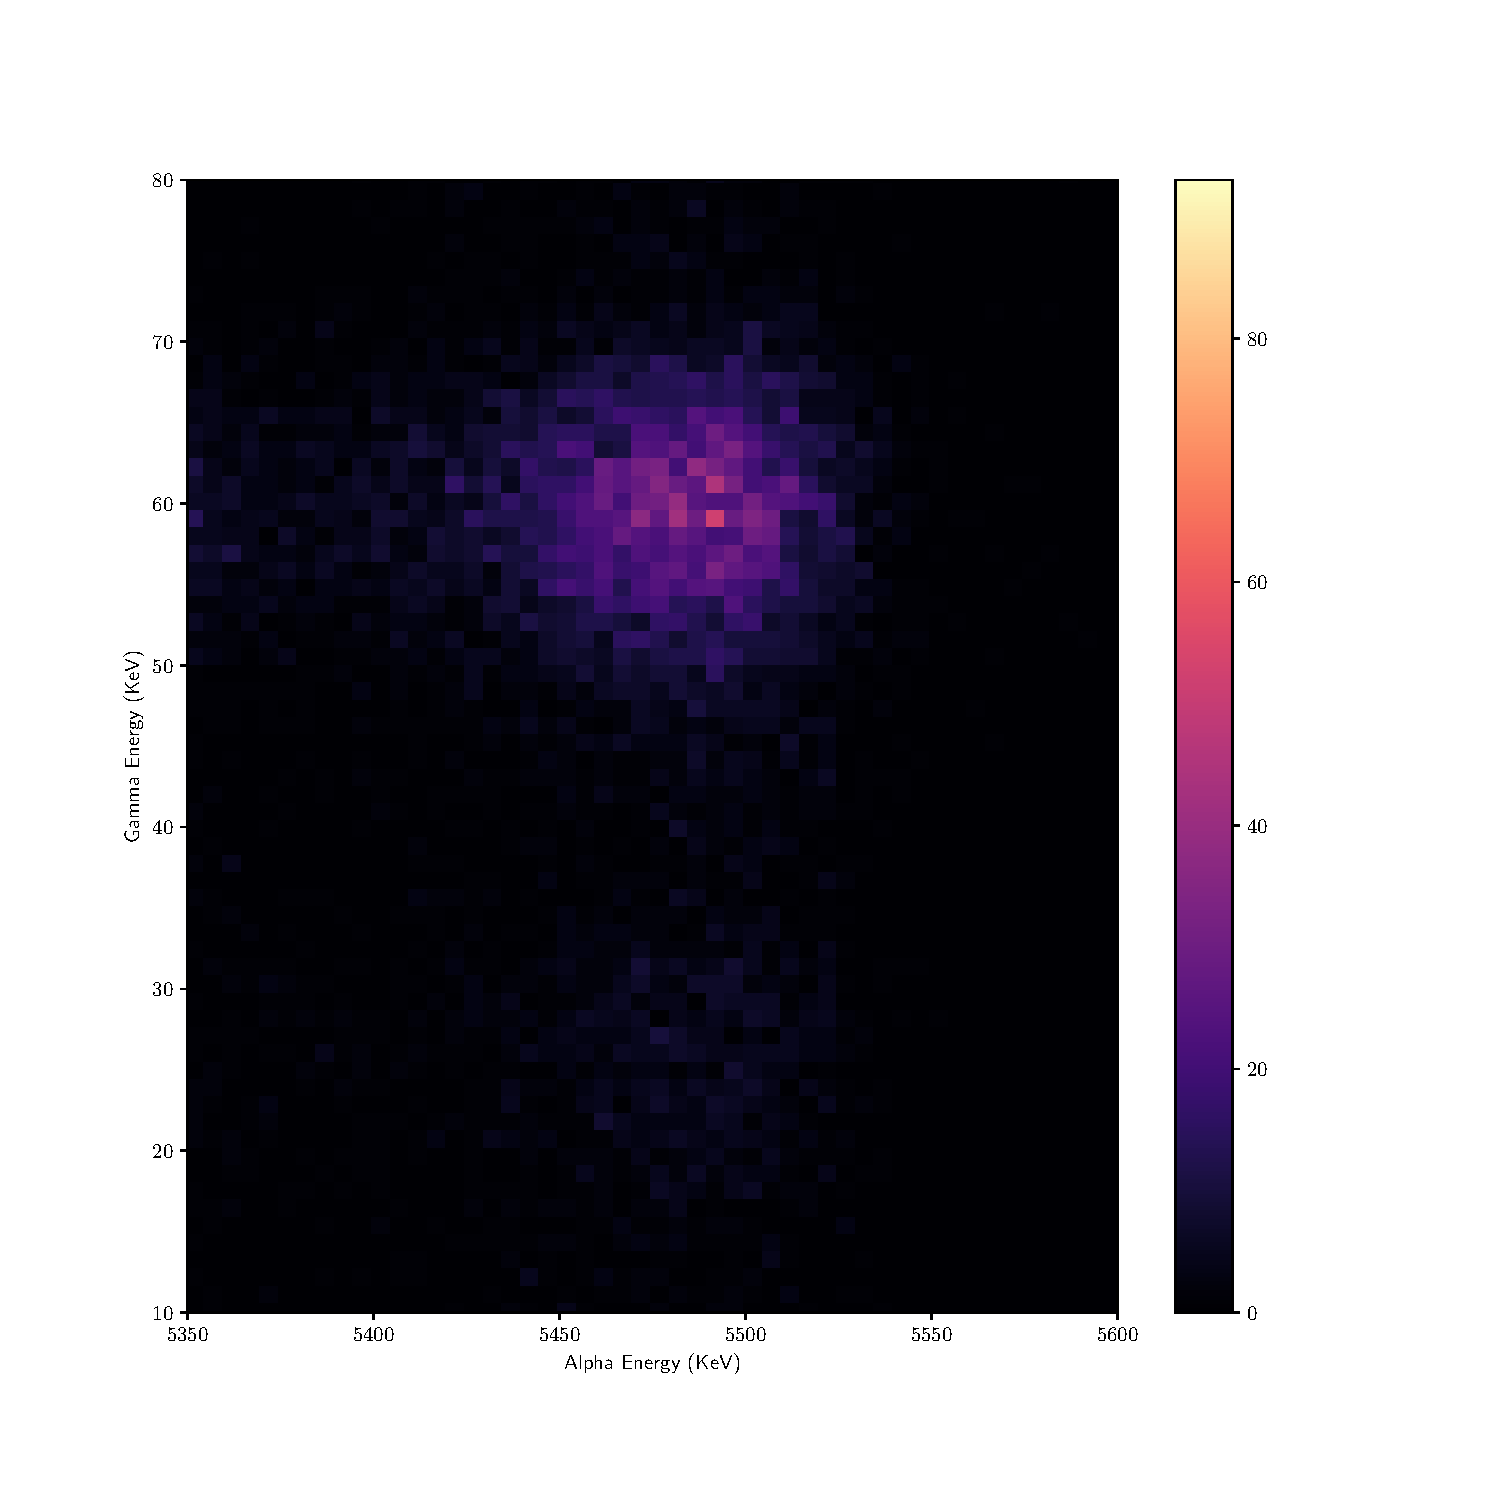
\includegraphics[width=\columnwidth]{images/hmap.pdf}
    \caption{Correlation heatmap}
\end{figure}

The graph below is a basic summation graph, where we are
looking at one of the energies, and seeing how it fares with
the other spectra's peak. We are looking at the peaks for
gamma. The correlated peak is the one with higher counts
than the uncorrelated peak, which was expected from the
graph before.
\begin{figure}[H]
	\centering
	\resizebox{0.8\columnwidth}{!}{%
		%% Creator: Matplotlib, PGF backend
%%
%% To include the figure in your LaTeX document, write
%%   \input{<filename>.pgf}
%%
%% Make sure the required packages are loaded in your preamble
%%   \usepackage{pgf}
%%
%% Figures using additional raster images can only be included by \input if
%% they are in the same directory as the main LaTeX file. For loading figures
%% from other directories you can use the `import` package
%%   \usepackage{import}
%%
%% and then include the figures with
%%   \import{<path to file>}{<filename>.pgf}
%%
%% Matplotlib used the following preamble
%%   \usepackage{fontspec}
%%   \setmainfont{DejaVuSerif.ttf}[Path=\detokenize{/home/spandan/.local/lib/python3.9/site-packages/matplotlib/mpl-data/fonts/ttf/}]
%%   \setsansfont{DejaVuSans.ttf}[Path=\detokenize{/home/spandan/.local/lib/python3.9/site-packages/matplotlib/mpl-data/fonts/ttf/}]
%%   \setmonofont{DejaVuSansMono.ttf}[Path=\detokenize{/home/spandan/.local/lib/python3.9/site-packages/matplotlib/mpl-data/fonts/ttf/}]
%%
\begingroup%
\makeatletter%
\begin{pgfpicture}%
\pgfpathrectangle{\pgfpointorigin}{\pgfqpoint{10.000000in}{10.000000in}}%
\pgfusepath{use as bounding box, clip}%
\begin{pgfscope}%
\pgfsetbuttcap%
\pgfsetmiterjoin%
\pgfsetlinewidth{0.000000pt}%
\definecolor{currentstroke}{rgb}{1.000000,1.000000,1.000000}%
\pgfsetstrokecolor{currentstroke}%
\pgfsetstrokeopacity{0.000000}%
\pgfsetdash{}{0pt}%
\pgfpathmoveto{\pgfqpoint{0.000000in}{0.000000in}}%
\pgfpathlineto{\pgfqpoint{10.000000in}{0.000000in}}%
\pgfpathlineto{\pgfqpoint{10.000000in}{10.000000in}}%
\pgfpathlineto{\pgfqpoint{0.000000in}{10.000000in}}%
\pgfpathclose%
\pgfusepath{}%
\end{pgfscope}%
\begin{pgfscope}%
\pgfsetbuttcap%
\pgfsetmiterjoin%
\definecolor{currentfill}{rgb}{1.000000,1.000000,1.000000}%
\pgfsetfillcolor{currentfill}%
\pgfsetlinewidth{0.000000pt}%
\definecolor{currentstroke}{rgb}{0.000000,0.000000,0.000000}%
\pgfsetstrokecolor{currentstroke}%
\pgfsetstrokeopacity{0.000000}%
\pgfsetdash{}{0pt}%
\pgfpathmoveto{\pgfqpoint{1.250000in}{1.250000in}}%
\pgfpathlineto{\pgfqpoint{9.000000in}{1.250000in}}%
\pgfpathlineto{\pgfqpoint{9.000000in}{8.800000in}}%
\pgfpathlineto{\pgfqpoint{1.250000in}{8.800000in}}%
\pgfpathclose%
\pgfusepath{fill}%
\end{pgfscope}%
\begin{pgfscope}%
\pgfpathrectangle{\pgfqpoint{1.250000in}{1.250000in}}{\pgfqpoint{7.750000in}{7.550000in}}%
\pgfusepath{clip}%
\pgfsetrectcap%
\pgfsetroundjoin%
\pgfsetlinewidth{1.505625pt}%
\definecolor{currentstroke}{rgb}{0.121569,0.466667,0.705882}%
\pgfsetstrokecolor{currentstroke}%
\pgfsetdash{}{0pt}%
\pgfpathmoveto{\pgfqpoint{1.236111in}{2.011123in}}%
\pgfpathlineto{\pgfqpoint{1.492225in}{2.206333in}}%
\pgfpathlineto{\pgfqpoint{1.822409in}{2.193750in}}%
\pgfpathlineto{\pgfqpoint{2.152593in}{2.533500in}}%
\pgfpathlineto{\pgfqpoint{2.482777in}{2.873250in}}%
\pgfpathlineto{\pgfqpoint{2.812961in}{3.666000in}}%
\pgfpathlineto{\pgfqpoint{3.143145in}{3.917667in}}%
\pgfpathlineto{\pgfqpoint{3.473329in}{4.144167in}}%
\pgfpathlineto{\pgfqpoint{3.803513in}{4.962083in}}%
\pgfpathlineto{\pgfqpoint{4.133697in}{5.956167in}}%
\pgfpathlineto{\pgfqpoint{4.463881in}{6.459500in}}%
\pgfpathlineto{\pgfqpoint{4.794065in}{6.774083in}}%
\pgfpathlineto{\pgfqpoint{5.124249in}{6.837000in}}%
\pgfpathlineto{\pgfqpoint{5.454433in}{8.120500in}}%
\pgfpathlineto{\pgfqpoint{5.784617in}{7.755583in}}%
\pgfpathlineto{\pgfqpoint{6.114801in}{7.755583in}}%
\pgfpathlineto{\pgfqpoint{6.444985in}{6.887333in}}%
\pgfpathlineto{\pgfqpoint{6.775169in}{6.837000in}}%
\pgfpathlineto{\pgfqpoint{7.105353in}{5.767417in}}%
\pgfpathlineto{\pgfqpoint{7.435537in}{5.163417in}}%
\pgfpathlineto{\pgfqpoint{7.765721in}{4.320333in}}%
\pgfpathlineto{\pgfqpoint{8.095905in}{4.068667in}}%
\pgfpathlineto{\pgfqpoint{8.426089in}{3.288500in}}%
\pgfpathlineto{\pgfqpoint{8.756273in}{2.445417in}}%
\pgfpathlineto{\pgfqpoint{9.013889in}{2.415963in}}%
\pgfusepath{stroke}%
\end{pgfscope}%
\begin{pgfscope}%
\pgfpathrectangle{\pgfqpoint{1.250000in}{1.250000in}}{\pgfqpoint{7.750000in}{7.550000in}}%
\pgfusepath{clip}%
\pgfsetrectcap%
\pgfsetroundjoin%
\pgfsetlinewidth{1.505625pt}%
\definecolor{currentstroke}{rgb}{1.000000,0.498039,0.054902}%
\pgfsetstrokecolor{currentstroke}%
\pgfsetdash{}{0pt}%
\pgfpathmoveto{\pgfqpoint{1.236111in}{1.475447in}}%
\pgfpathlineto{\pgfqpoint{1.492225in}{1.602333in}}%
\pgfpathlineto{\pgfqpoint{1.822409in}{1.552000in}}%
\pgfpathlineto{\pgfqpoint{2.152593in}{1.602333in}}%
\pgfpathlineto{\pgfqpoint{2.482777in}{1.791083in}}%
\pgfpathlineto{\pgfqpoint{2.812961in}{1.879167in}}%
\pgfpathlineto{\pgfqpoint{3.143145in}{1.841417in}}%
\pgfpathlineto{\pgfqpoint{3.473329in}{2.093083in}}%
\pgfpathlineto{\pgfqpoint{3.803513in}{2.030167in}}%
\pgfpathlineto{\pgfqpoint{4.133697in}{2.168583in}}%
\pgfpathlineto{\pgfqpoint{4.463881in}{2.193750in}}%
\pgfpathlineto{\pgfqpoint{4.794065in}{1.904333in}}%
\pgfpathlineto{\pgfqpoint{5.124249in}{2.458000in}}%
\pgfpathlineto{\pgfqpoint{5.454433in}{2.206333in}}%
\pgfpathlineto{\pgfqpoint{5.784617in}{2.432833in}}%
\pgfpathlineto{\pgfqpoint{6.114801in}{2.168583in}}%
\pgfpathlineto{\pgfqpoint{6.444985in}{2.244083in}}%
\pgfpathlineto{\pgfqpoint{6.775169in}{2.281833in}}%
\pgfpathlineto{\pgfqpoint{7.105353in}{1.803667in}}%
\pgfpathlineto{\pgfqpoint{7.435537in}{1.816250in}}%
\pgfpathlineto{\pgfqpoint{7.765721in}{1.677833in}}%
\pgfpathlineto{\pgfqpoint{8.095905in}{1.665250in}}%
\pgfpathlineto{\pgfqpoint{8.426089in}{1.602333in}}%
\pgfpathlineto{\pgfqpoint{8.756273in}{1.577167in}}%
\pgfpathlineto{\pgfqpoint{9.013889in}{1.606620in}}%
\pgfusepath{stroke}%
\end{pgfscope}%
\begin{pgfscope}%
\pgfsetrectcap%
\pgfsetmiterjoin%
\pgfsetlinewidth{0.803000pt}%
\definecolor{currentstroke}{rgb}{0.000000,0.000000,0.000000}%
\pgfsetstrokecolor{currentstroke}%
\pgfsetdash{}{0pt}%
\pgfpathmoveto{\pgfqpoint{1.250000in}{1.250000in}}%
\pgfpathlineto{\pgfqpoint{1.250000in}{8.800000in}}%
\pgfusepath{stroke}%
\end{pgfscope}%
\begin{pgfscope}%
\pgfsetrectcap%
\pgfsetmiterjoin%
\pgfsetlinewidth{0.803000pt}%
\definecolor{currentstroke}{rgb}{0.000000,0.000000,0.000000}%
\pgfsetstrokecolor{currentstroke}%
\pgfsetdash{}{0pt}%
\pgfpathmoveto{\pgfqpoint{9.000000in}{1.250000in}}%
\pgfpathlineto{\pgfqpoint{9.000000in}{8.800000in}}%
\pgfusepath{stroke}%
\end{pgfscope}%
\begin{pgfscope}%
\pgfsetrectcap%
\pgfsetmiterjoin%
\pgfsetlinewidth{0.803000pt}%
\definecolor{currentstroke}{rgb}{0.000000,0.000000,0.000000}%
\pgfsetstrokecolor{currentstroke}%
\pgfsetdash{}{0pt}%
\pgfpathmoveto{\pgfqpoint{1.250000in}{1.250000in}}%
\pgfpathlineto{\pgfqpoint{9.000000in}{1.250000in}}%
\pgfusepath{stroke}%
\end{pgfscope}%
\begin{pgfscope}%
\pgfsetrectcap%
\pgfsetmiterjoin%
\pgfsetlinewidth{0.803000pt}%
\definecolor{currentstroke}{rgb}{0.000000,0.000000,0.000000}%
\pgfsetstrokecolor{currentstroke}%
\pgfsetdash{}{0pt}%
\pgfpathmoveto{\pgfqpoint{1.250000in}{8.800000in}}%
\pgfpathlineto{\pgfqpoint{9.000000in}{8.800000in}}%
\pgfusepath{stroke}%
\end{pgfscope}%
\begin{pgfscope}%
\pgfsetbuttcap%
\pgfsetmiterjoin%
\definecolor{currentfill}{rgb}{1.000000,1.000000,1.000000}%
\pgfsetfillcolor{currentfill}%
\pgfsetfillopacity{0.800000}%
\pgfsetlinewidth{1.003750pt}%
\definecolor{currentstroke}{rgb}{0.800000,0.800000,0.800000}%
\pgfsetstrokecolor{currentstroke}%
\pgfsetstrokeopacity{0.800000}%
\pgfsetdash{}{0pt}%
\pgfpathmoveto{\pgfqpoint{7.191718in}{8.281174in}}%
\pgfpathlineto{\pgfqpoint{8.902778in}{8.281174in}}%
\pgfpathquadraticcurveto{\pgfqpoint{8.930556in}{8.281174in}}{\pgfqpoint{8.930556in}{8.308952in}}%
\pgfpathlineto{\pgfqpoint{8.930556in}{8.702778in}}%
\pgfpathquadraticcurveto{\pgfqpoint{8.930556in}{8.730556in}}{\pgfqpoint{8.902778in}{8.730556in}}%
\pgfpathlineto{\pgfqpoint{7.191718in}{8.730556in}}%
\pgfpathquadraticcurveto{\pgfqpoint{7.163940in}{8.730556in}}{\pgfqpoint{7.163940in}{8.702778in}}%
\pgfpathlineto{\pgfqpoint{7.163940in}{8.308952in}}%
\pgfpathquadraticcurveto{\pgfqpoint{7.163940in}{8.281174in}}{\pgfqpoint{7.191718in}{8.281174in}}%
\pgfpathclose%
\pgfusepath{stroke,fill}%
\end{pgfscope}%
\begin{pgfscope}%
\pgfsetrectcap%
\pgfsetroundjoin%
\pgfsetlinewidth{1.505625pt}%
\definecolor{currentstroke}{rgb}{0.121569,0.466667,0.705882}%
\pgfsetstrokecolor{currentstroke}%
\pgfsetdash{}{0pt}%
\pgfpathmoveto{\pgfqpoint{7.219496in}{8.618088in}}%
\pgfpathlineto{\pgfqpoint{7.497274in}{8.618088in}}%
\pgfusepath{stroke}%
\end{pgfscope}%
\begin{pgfscope}%
\definecolor{textcolor}{rgb}{0.000000,0.000000,0.000000}%
\pgfsetstrokecolor{textcolor}%
\pgfsetfillcolor{textcolor}%
\pgftext[x=7.608385in,y=8.569477in,left,base]{\color{textcolor}\sffamily\fontsize{10.000000}{12.000000}\selectfont correlated peak}%
\end{pgfscope}%
\begin{pgfscope}%
\pgfsetrectcap%
\pgfsetroundjoin%
\pgfsetlinewidth{1.505625pt}%
\definecolor{currentstroke}{rgb}{1.000000,0.498039,0.054902}%
\pgfsetstrokecolor{currentstroke}%
\pgfsetdash{}{0pt}%
\pgfpathmoveto{\pgfqpoint{7.219496in}{8.414231in}}%
\pgfpathlineto{\pgfqpoint{7.497274in}{8.414231in}}%
\pgfusepath{stroke}%
\end{pgfscope}%
\begin{pgfscope}%
\definecolor{textcolor}{rgb}{0.000000,0.000000,0.000000}%
\pgfsetstrokecolor{textcolor}%
\pgfsetfillcolor{textcolor}%
\pgftext[x=7.608385in,y=8.365620in,left,base]{\color{textcolor}\sffamily\fontsize{10.000000}{12.000000}\selectfont uncorrelated peak}%
\end{pgfscope}%
\end{pgfpicture}%
\makeatother%
\endgroup%

	}
    \caption{Gated correlation for both the gamma peaks}
\end{figure}
We can do the correlation delay measurements with a FPGA,
but given that we do not have enough equipment for that, we
couldn't attempt that part of the experiment. The
correlation delay can be then used to find the background
and be used to find out the actual correlation heatmap.

Some other calculations can then be done to estimate the
half life of the metastable state, which our primary
reference did, and proved to a high accuracy that the
experiment is possible.

\section{Conclusion}
We were able to setup and demonstrate alpha gamma
coincidence for $^{241}$Am. The graphs came out to be as
expected, and the experiment may be considered a success.

\section{References}
\begin{enumerate}
    \item \fullcite{vret}
    \item \fullcite{filipe}
    \item \fullcite{fpga}
    \item \fullcite{alterra}
\end{enumerate}
\end{multicols*}
\clearpage
\end{document}
